% !TEX root = thesis.tex

%%
%%
%% results tables and figures appendix
%%
%%

%%
%% Section containing all uniform risk on uniform population
%%
\section{Uniform risk on a uniform population}
\label{sec:app:results_unif_unif}

%%
%% Tables and figures for uniform population of 10,000, uniform risk of factor 50
%%
\graphicspath{{./results/unif_50_unif/}}
\makeatletter
\def\input@path{{./results/unif_50_unif/}}
\makeatother

\begin{table}[H]
        \centering
    \tiny
    \begin{subtable}[t]{0.5\textwidth}
        \centering
        \subcaption{Means} 
        % latex table generated in R 3.4.2 by xtable 1.8-2 package
% Sat Feb 17 16:44:44 2018
\begin{tabular}{lrrr}
  \hline
 & Oracle & Silverman & CV \\ 
  \hline
MISE & 0.000053 & 0.000083 & 0.000080 \\ 
  Relative MISE & 0.002028 & 0.003195 & 0.003047 \\ 
  Normalized MISE & 0.000026 & 0.000042 & 0.000040 \\ 
  MIAE & 0.003914 & 0.004863 & 0.004653 \\ 
  Relative MIAE & 0.024227 & 0.030102 & 0.028802 \\ 
  Max Error & 0.033855 & 0.049415 & 0.045884 \\ 
  Peak bias & -0.016050 & 0.010816 & -0.002953 \\ 
  Relative Peak bias & -0.099339 & 0.066949 & -0.018278 \\ 
  Peak drift & 0.223424 & 0.357624 & 0.284159 \\ 
  Relative Peak drift & 0.031918 & 0.051089 & 0.040594 \\ 
  Centroid bias & -0.017140 & -0.000902 & -0.013918 \\ 
  Relative Centroid bias & -0.106087 & -0.005583 & -0.086149 \\ 
  Centroid drift & 0.149249 & 0.159867 & 0.152694 \\ 
  Relative Centroid drift & 0.021321 & 0.022838 & 0.021813 \\ 
   \hline
\end{tabular}

    \end{subtable}%
    \begin{subtable}[t]{0.5\textwidth}
        \centering
        \subcaption{Standard deviations} 
        % latex table generated in R 3.4.3 by xtable 1.8-2 package
% Sun Apr 15 09:09:45 2018
\begin{tabular}{lrrr}
  \toprule
 & Oracle & Silverman & CV \\ 
  \midrule
MISE & 0.000014 & 0.000014 & 0.000021 \\ 
  Relative MISE & 0.001962 & 0.002039 & 0.003010 \\ 
  Normalized MISE & 0.344229 & 0.357804 & 0.528098 \\ 
  MIAE & 0.000689 & 0.000597 & 0.000961 \\ 
  Relative MIAE & 0.008228 & 0.007121 & 0.011473 \\ 
  Normalized MIAE & 0.000003 & 0.000003 & 0.000005 \\ 
  Supremum error & 0.005321 & 0.006343 & 0.008947 \\ 
  Normalized Sup error & 0.000027 & 0.000032 & 0.000045 \\ 
  Peak bias & 0.008408 & 0.012518 & 0.015040 \\ 
  Relative Peak bias & 0.100360 & 0.149419 & 0.179526 \\ 
  Peak drift & 0.186254 & 0.253752 & 0.225627 \\ 
  Relative Peak drift & 0.026608 & 0.036250 & 0.032232 \\ 
  Centroid bias & 0.008526 & 0.013326 & 0.013412 \\ 
  Relative Centroid bias & 0.101772 & 0.159063 & 0.160095 \\ 
  Centroid drift & 0.142123 & 0.159726 & 0.144847 \\ 
  Relative Centroid drift & 0.020303 & 0.022818 & 0.020692 \\ 
   \bottomrule
\end{tabular}

    \end{subtable}

    \caption[]{Error rates for uniform population of 10,000, uniform risk of factor 50}
    \label{tab:mean_error_rates:unif_50_unif}
\end{table}

\begin{figure}[H]
        \centering
    \begin{subfigure}[t]{0.33\textwidth}
    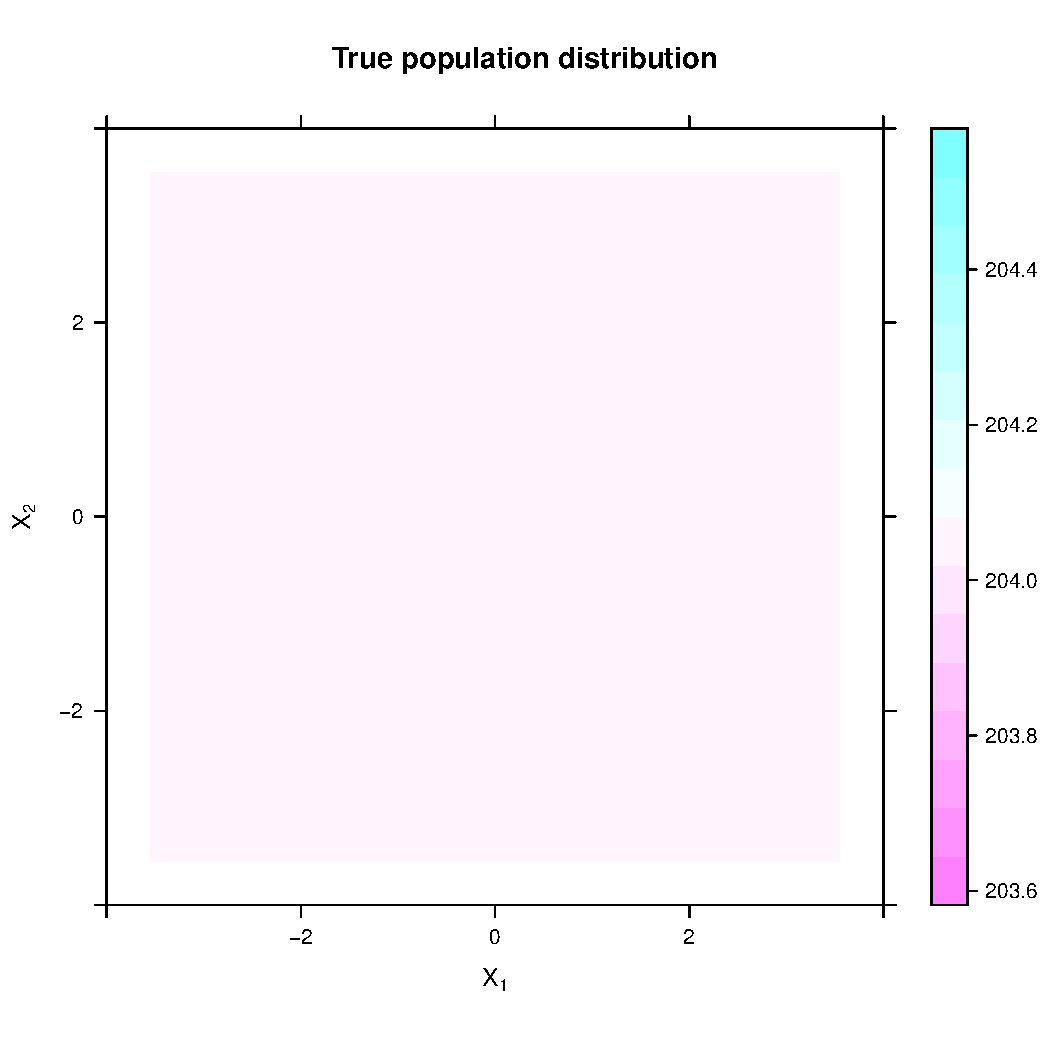
\includegraphics[width=\textwidth]{output/population-heatmap}
    \subcaption{Population distribution}
    \end{subfigure}
    \begin{subfigure}[t]{0.33\textwidth}
    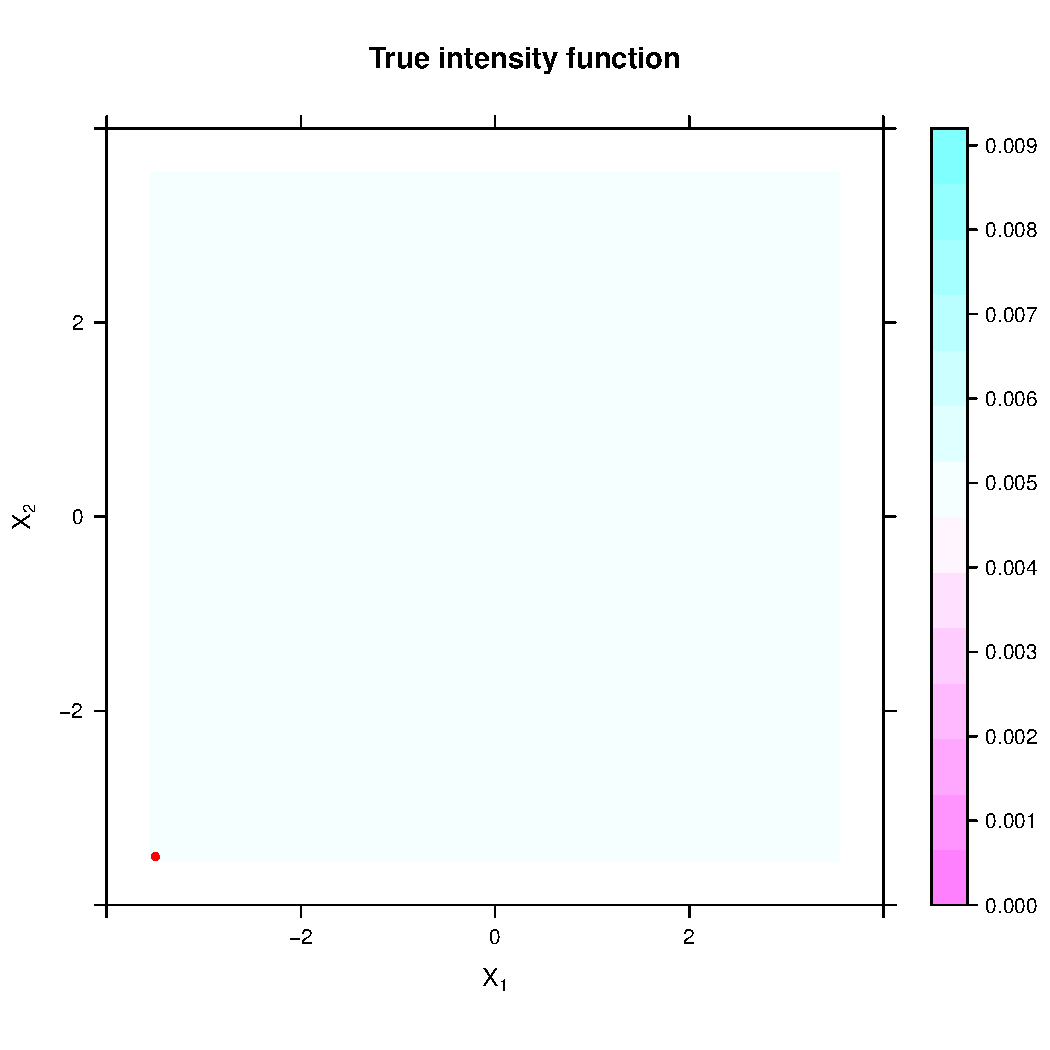
\includegraphics[width=\textwidth]{output/true_intensity_heatmap}
    \subcaption{True risk function}
    \end{subfigure}%
    \begin{subfigure}[t]{0.32\textwidth}
    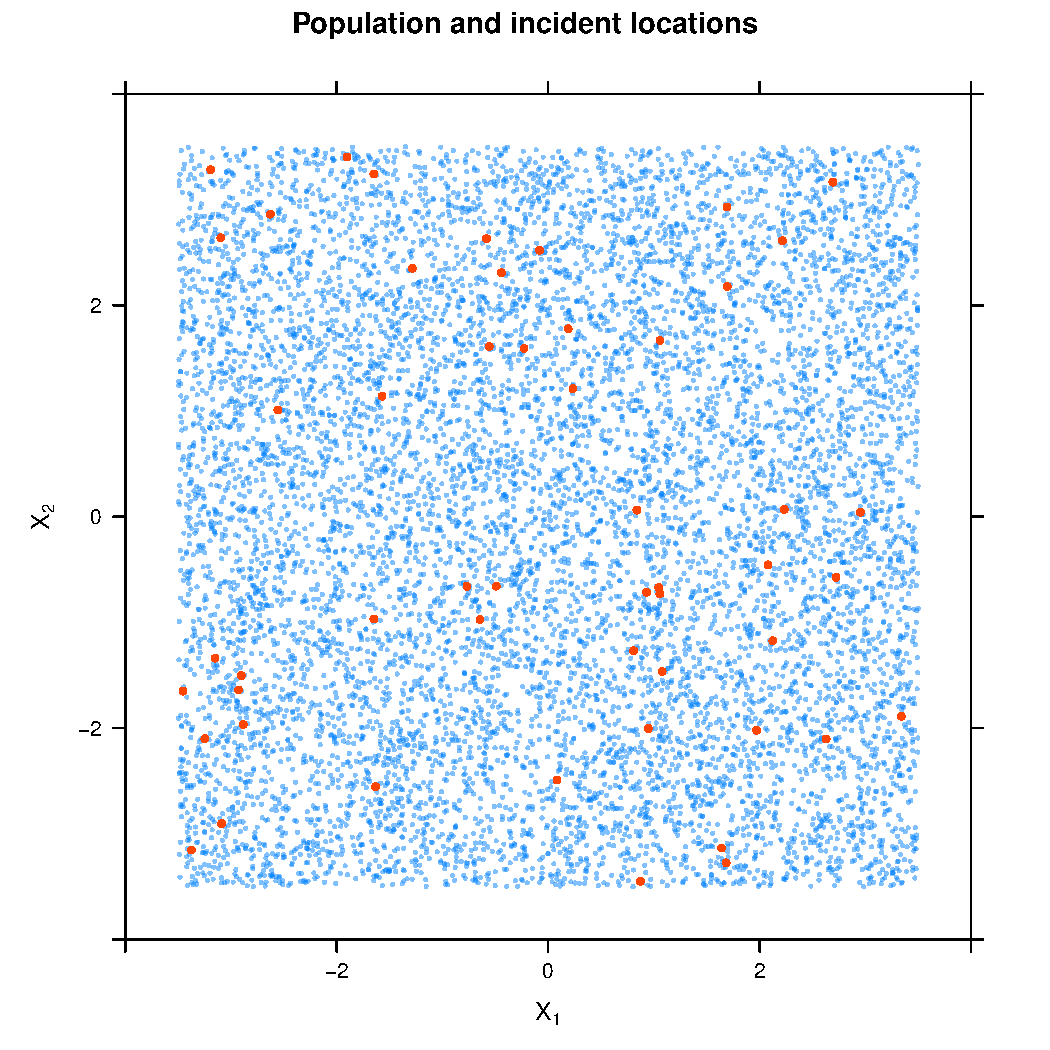
\includegraphics[width=\textwidth]{output/population_and_incidents_scatter}
    \subcaption{Population points (gray) with incidents (black)}
    \end{subfigure}%

    \caption[]{Population distribution (a), true risk function (b), and sample population with incidents (c) for uniform population of 10,000, uniform risk of factor 50}
    \label{fig:distributions:unif_50_unif}    
\end{figure}


%%
%% Tables and figures for uniform population of 10,000, uniform risk of factor 100
%%
\graphicspath{{./results/unif_100_unif/}}
\makeatletter
\def\input@path{{./results/unif_100_unif/}}
\makeatother

\begin{table}[H]
    \centering
    \tiny
    \begin{subtable}[t]{0.5\textwidth}
        \centering
        \subcaption{Means} 
        % latex table generated in R 3.4.2 by xtable 1.8-2 package
% Sat Feb 17 16:44:44 2018
\begin{tabular}{lrrr}
  \hline
 & Oracle & Silverman & CV \\ 
  \hline
MISE & 0.000053 & 0.000083 & 0.000080 \\ 
  Relative MISE & 0.002028 & 0.003195 & 0.003047 \\ 
  Normalized MISE & 0.000026 & 0.000042 & 0.000040 \\ 
  MIAE & 0.003914 & 0.004863 & 0.004653 \\ 
  Relative MIAE & 0.024227 & 0.030102 & 0.028802 \\ 
  Max Error & 0.033855 & 0.049415 & 0.045884 \\ 
  Peak bias & -0.016050 & 0.010816 & -0.002953 \\ 
  Relative Peak bias & -0.099339 & 0.066949 & -0.018278 \\ 
  Peak drift & 0.223424 & 0.357624 & 0.284159 \\ 
  Relative Peak drift & 0.031918 & 0.051089 & 0.040594 \\ 
  Centroid bias & -0.017140 & -0.000902 & -0.013918 \\ 
  Relative Centroid bias & -0.106087 & -0.005583 & -0.086149 \\ 
  Centroid drift & 0.149249 & 0.159867 & 0.152694 \\ 
  Relative Centroid drift & 0.021321 & 0.022838 & 0.021813 \\ 
   \hline
\end{tabular}

    \end{subtable}%
    \begin{subtable}[t]{0.5\textwidth}
        \centering
        \subcaption{Standard deviations} 
        % latex table generated in R 3.4.3 by xtable 1.8-2 package
% Sun Apr 15 09:09:45 2018
\begin{tabular}{lrrr}
  \toprule
 & Oracle & Silverman & CV \\ 
  \midrule
MISE & 0.000014 & 0.000014 & 0.000021 \\ 
  Relative MISE & 0.001962 & 0.002039 & 0.003010 \\ 
  Normalized MISE & 0.344229 & 0.357804 & 0.528098 \\ 
  MIAE & 0.000689 & 0.000597 & 0.000961 \\ 
  Relative MIAE & 0.008228 & 0.007121 & 0.011473 \\ 
  Normalized MIAE & 0.000003 & 0.000003 & 0.000005 \\ 
  Supremum error & 0.005321 & 0.006343 & 0.008947 \\ 
  Normalized Sup error & 0.000027 & 0.000032 & 0.000045 \\ 
  Peak bias & 0.008408 & 0.012518 & 0.015040 \\ 
  Relative Peak bias & 0.100360 & 0.149419 & 0.179526 \\ 
  Peak drift & 0.186254 & 0.253752 & 0.225627 \\ 
  Relative Peak drift & 0.026608 & 0.036250 & 0.032232 \\ 
  Centroid bias & 0.008526 & 0.013326 & 0.013412 \\ 
  Relative Centroid bias & 0.101772 & 0.159063 & 0.160095 \\ 
  Centroid drift & 0.142123 & 0.159726 & 0.144847 \\ 
  Relative Centroid drift & 0.020303 & 0.022818 & 0.020692 \\ 
   \bottomrule
\end{tabular}

    \end{subtable}

\caption[]{Error rates for uniform population of 10,000, uniform risk of factor 100}
\label{tab:mean_error_rates:unif_100_unif}
\end{table}

\begin{figure}[H]
        \centering
    \begin{subfigure}[t]{0.33\textwidth}
    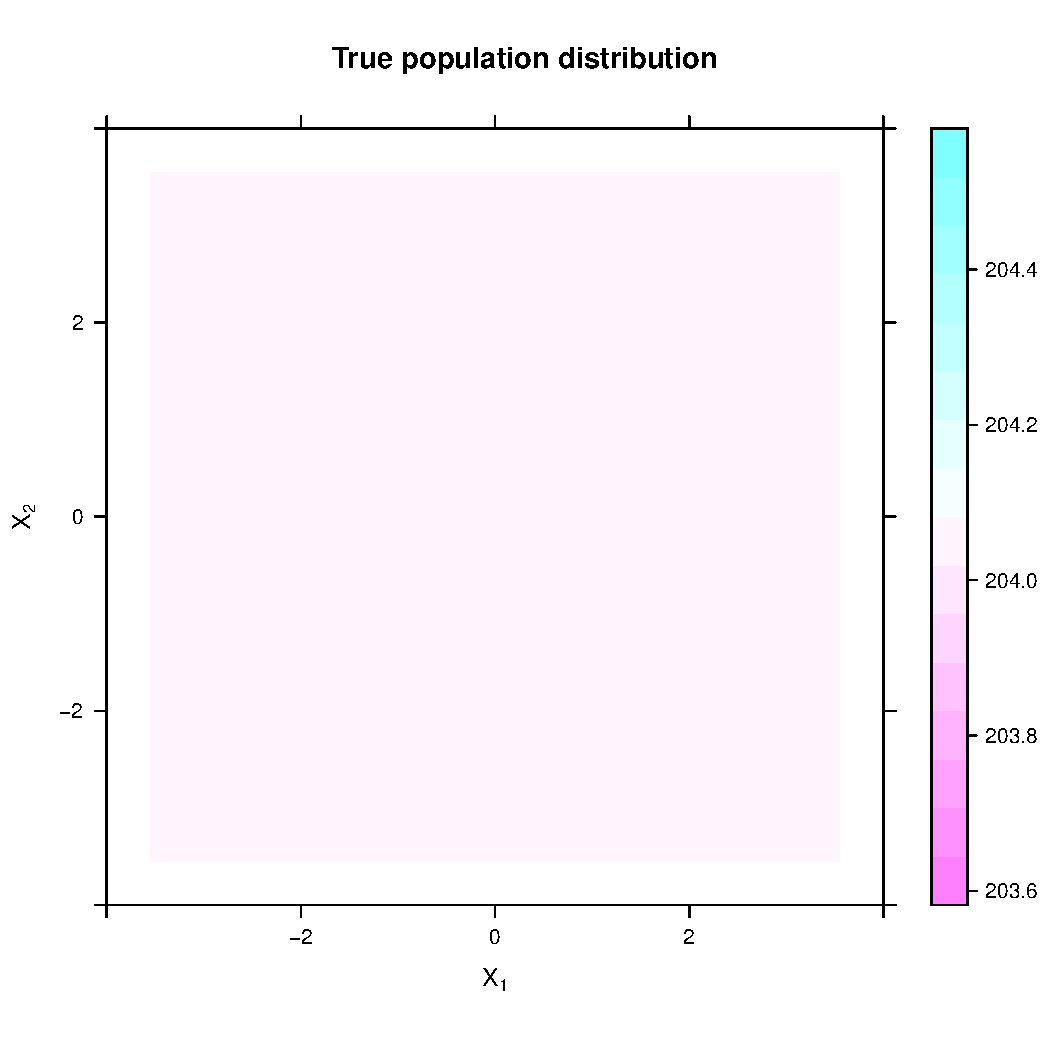
\includegraphics[width=\textwidth]{output/population-heatmap}
    \subcaption{Population distribution}
    \end{subfigure}
    \begin{subfigure}[t]{0.33\textwidth}
    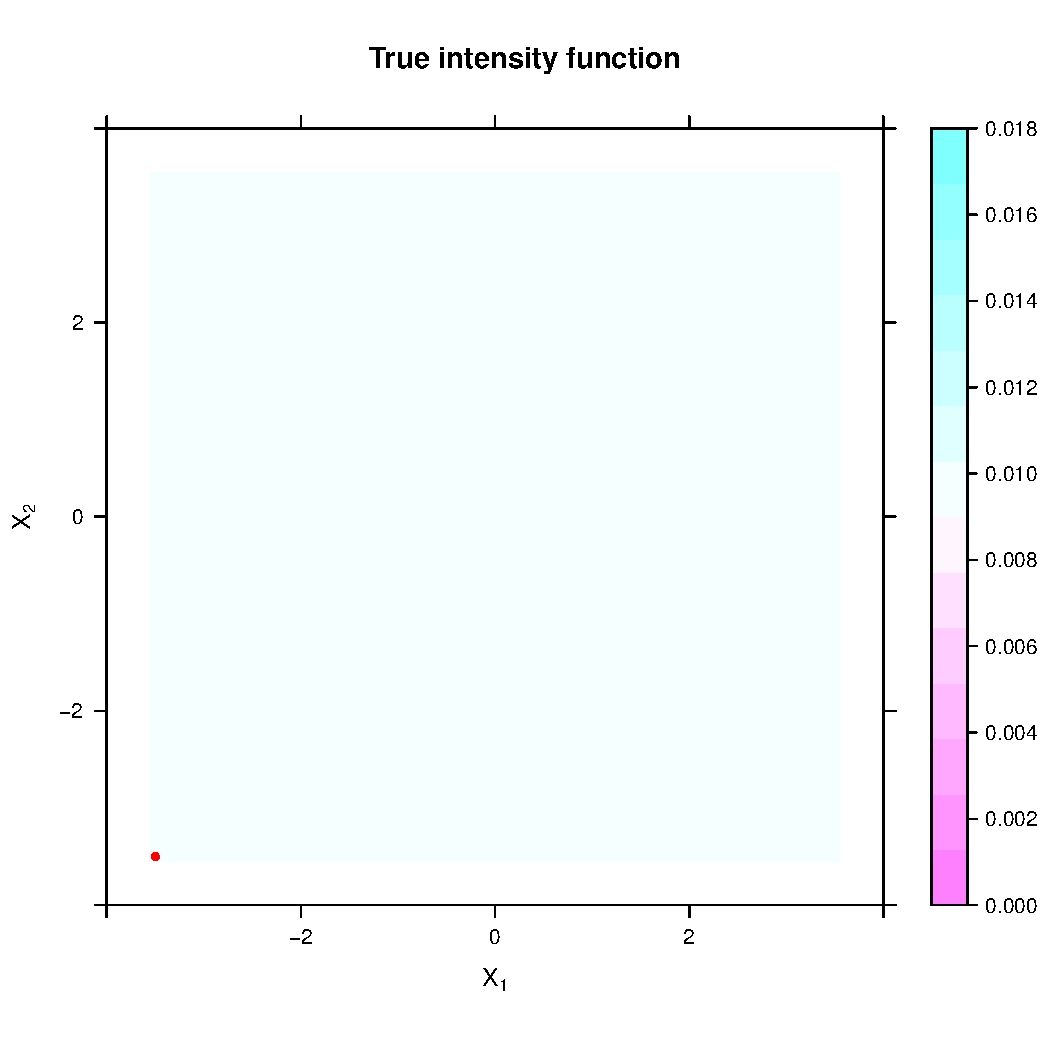
\includegraphics[width=\textwidth]{output/true_intensity_heatmap}
    \subcaption{True risk function}
    \end{subfigure}%
    \begin{subfigure}[t]{0.32\textwidth}
    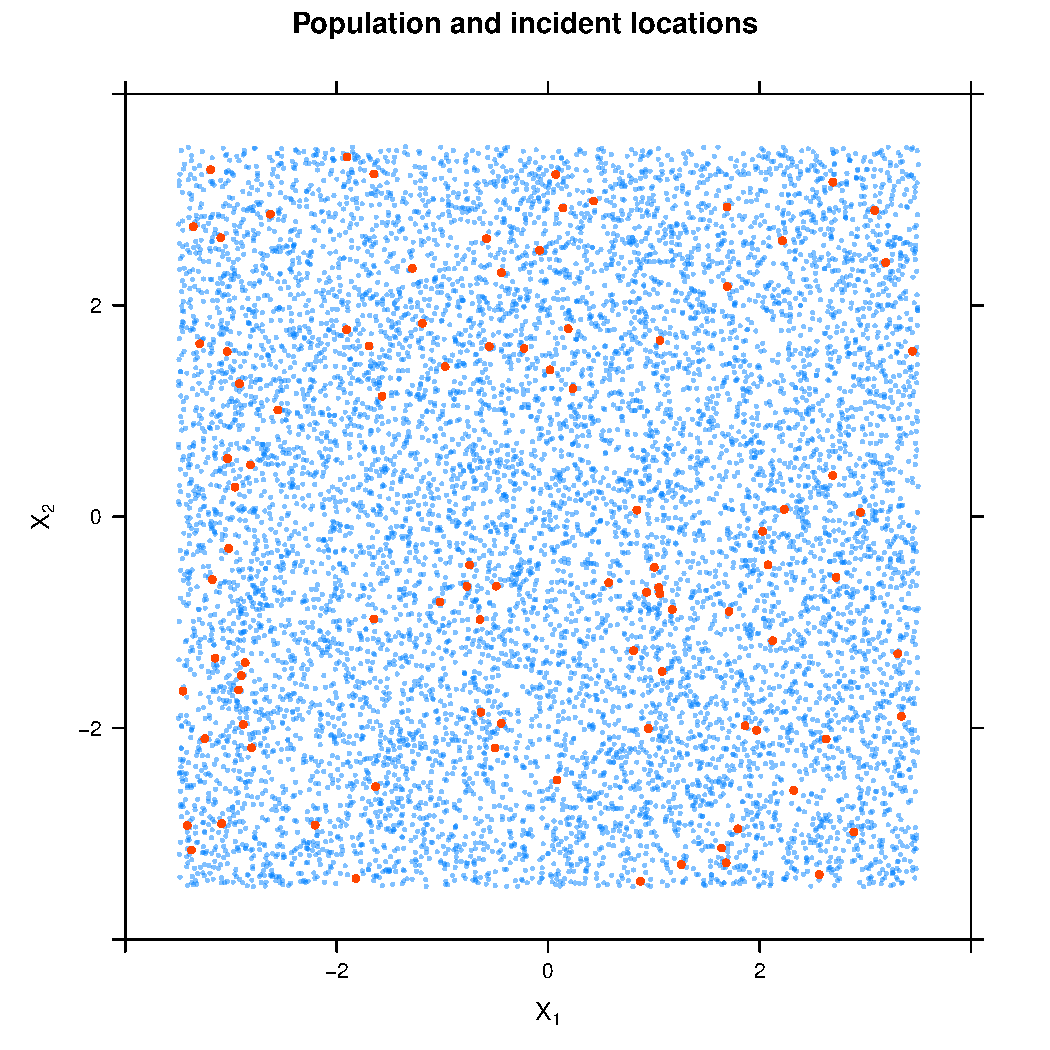
\includegraphics[width=\textwidth]{output/population_and_incidents_scatter}
    \subcaption{Population points (gray) with incidents (black)}
    \end{subfigure}%

    \caption[]{Population distribution (a), true risk function (b), and sample population with incidents (c) for uniform population of 10,000, uniform risk of factor 100}
    \label{fig:distributions:unif_100_unif}    
\end{figure}


%%
%% Tables and figures for uniform population of 10,000, uniform risk of factor 200
%%
\graphicspath{{./results/unif_200_unif/}}
\makeatletter
\def\input@path{{./results/unif_200_unif/}}
\makeatother

\begin{table}[H]
    \centering
    \tiny
    \begin{subtable}[t]{0.5\textwidth}
        \centering
        \subcaption{Means} 
        % latex table generated in R 3.4.2 by xtable 1.8-2 package
% Sat Feb 17 16:44:44 2018
\begin{tabular}{lrrr}
  \hline
 & Oracle & Silverman & CV \\ 
  \hline
MISE & 0.000053 & 0.000083 & 0.000080 \\ 
  Relative MISE & 0.002028 & 0.003195 & 0.003047 \\ 
  Normalized MISE & 0.000026 & 0.000042 & 0.000040 \\ 
  MIAE & 0.003914 & 0.004863 & 0.004653 \\ 
  Relative MIAE & 0.024227 & 0.030102 & 0.028802 \\ 
  Max Error & 0.033855 & 0.049415 & 0.045884 \\ 
  Peak bias & -0.016050 & 0.010816 & -0.002953 \\ 
  Relative Peak bias & -0.099339 & 0.066949 & -0.018278 \\ 
  Peak drift & 0.223424 & 0.357624 & 0.284159 \\ 
  Relative Peak drift & 0.031918 & 0.051089 & 0.040594 \\ 
  Centroid bias & -0.017140 & -0.000902 & -0.013918 \\ 
  Relative Centroid bias & -0.106087 & -0.005583 & -0.086149 \\ 
  Centroid drift & 0.149249 & 0.159867 & 0.152694 \\ 
  Relative Centroid drift & 0.021321 & 0.022838 & 0.021813 \\ 
   \hline
\end{tabular}

    \end{subtable}%
    \begin{subtable}[t]{0.5\textwidth}
        \centering
        \subcaption{Standard deviations} 
        % latex table generated in R 3.4.3 by xtable 1.8-2 package
% Sun Apr 15 09:09:45 2018
\begin{tabular}{lrrr}
  \toprule
 & Oracle & Silverman & CV \\ 
  \midrule
MISE & 0.000014 & 0.000014 & 0.000021 \\ 
  Relative MISE & 0.001962 & 0.002039 & 0.003010 \\ 
  Normalized MISE & 0.344229 & 0.357804 & 0.528098 \\ 
  MIAE & 0.000689 & 0.000597 & 0.000961 \\ 
  Relative MIAE & 0.008228 & 0.007121 & 0.011473 \\ 
  Normalized MIAE & 0.000003 & 0.000003 & 0.000005 \\ 
  Supremum error & 0.005321 & 0.006343 & 0.008947 \\ 
  Normalized Sup error & 0.000027 & 0.000032 & 0.000045 \\ 
  Peak bias & 0.008408 & 0.012518 & 0.015040 \\ 
  Relative Peak bias & 0.100360 & 0.149419 & 0.179526 \\ 
  Peak drift & 0.186254 & 0.253752 & 0.225627 \\ 
  Relative Peak drift & 0.026608 & 0.036250 & 0.032232 \\ 
  Centroid bias & 0.008526 & 0.013326 & 0.013412 \\ 
  Relative Centroid bias & 0.101772 & 0.159063 & 0.160095 \\ 
  Centroid drift & 0.142123 & 0.159726 & 0.144847 \\ 
  Relative Centroid drift & 0.020303 & 0.022818 & 0.020692 \\ 
   \bottomrule
\end{tabular}

    \end{subtable}

\caption[]{Error rates for uniform population of 10,000, uniform risk of factor 200}
\label{tab:mean_error_rates:unif_200_unif}
\end{table}

\begin{figure}[H]
        \centering
    \begin{subfigure}[t]{0.33\textwidth}
    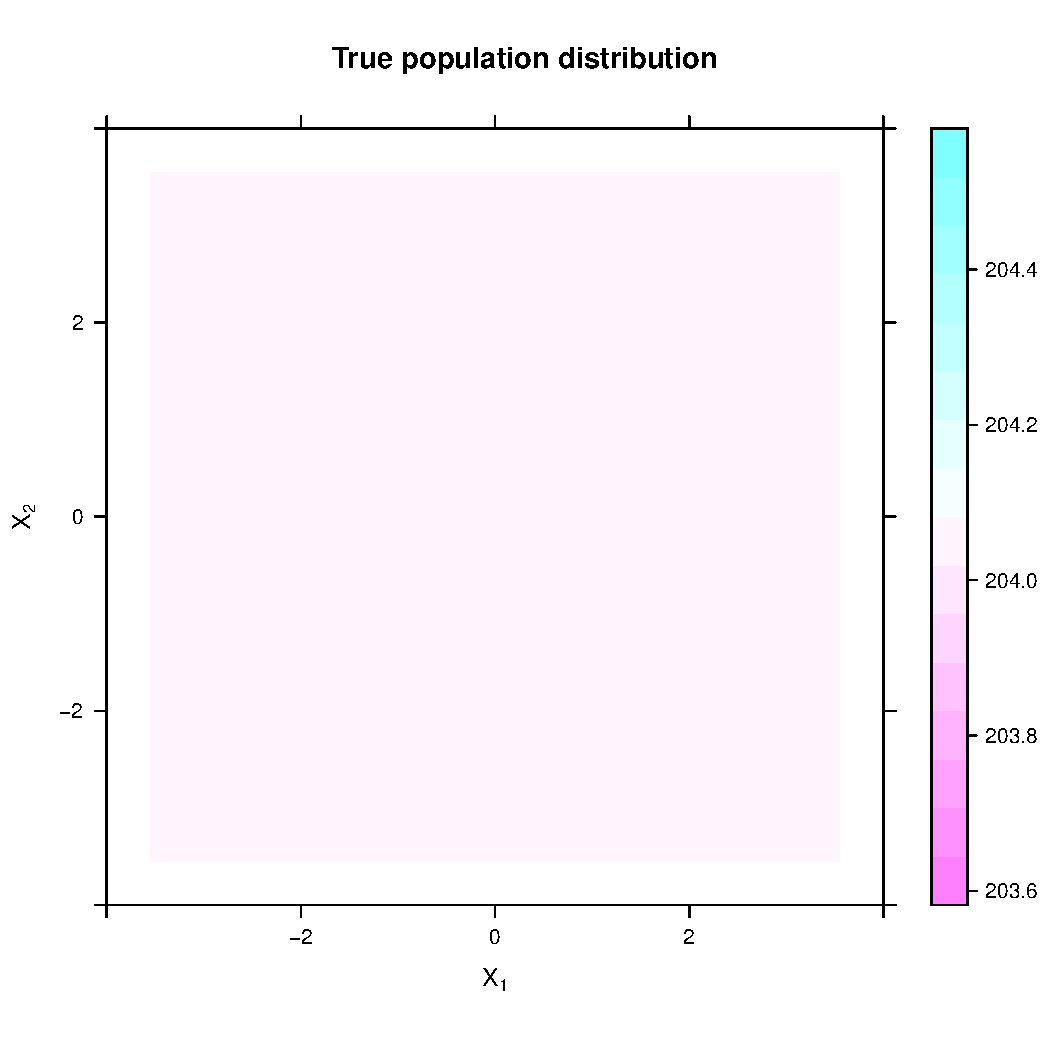
\includegraphics[width=\textwidth]{output/population-heatmap}
    \subcaption{Population distribution}
    \end{subfigure}
    \begin{subfigure}[t]{0.33\textwidth}
    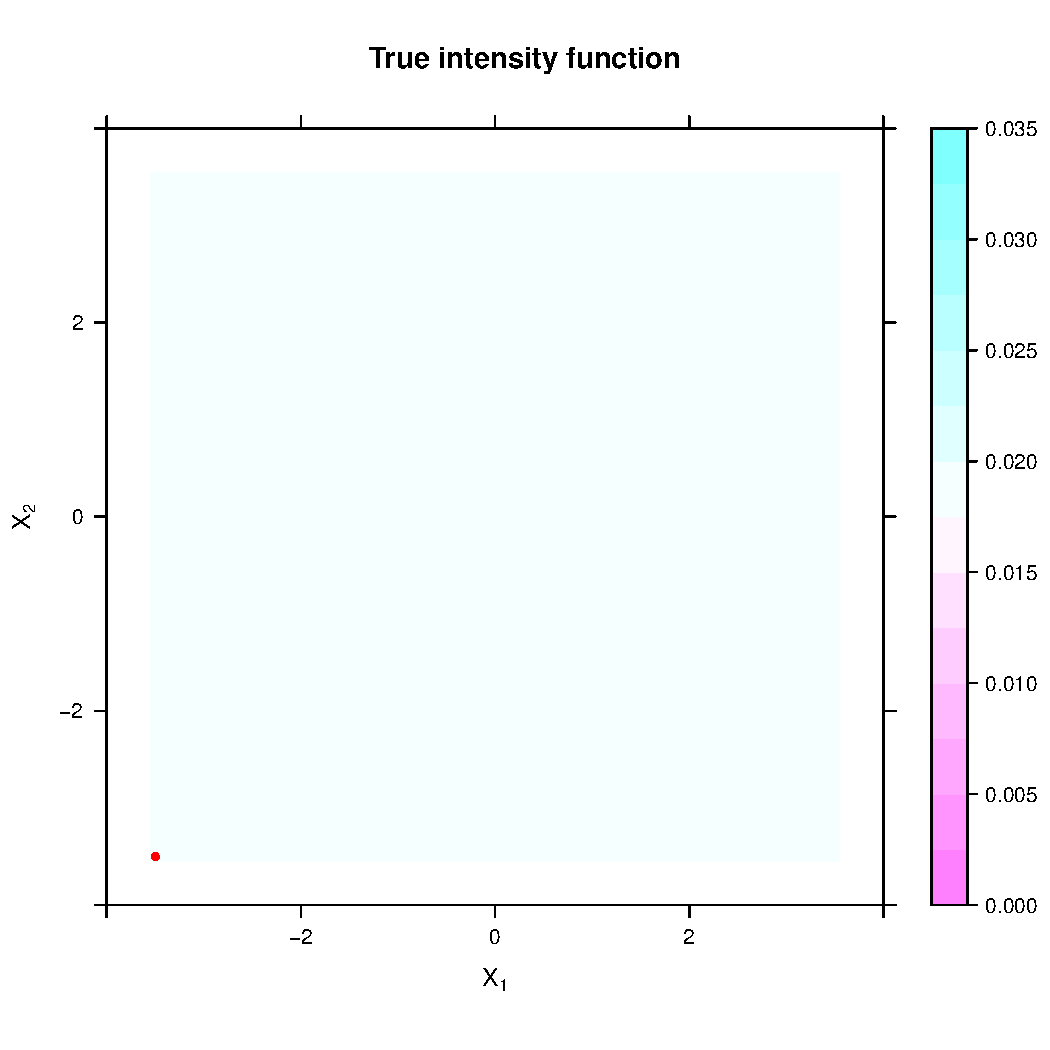
\includegraphics[width=\textwidth]{output/true_intensity_heatmap}
    \subcaption{True risk function}
    \end{subfigure}%
    \begin{subfigure}[t]{0.32\textwidth}
    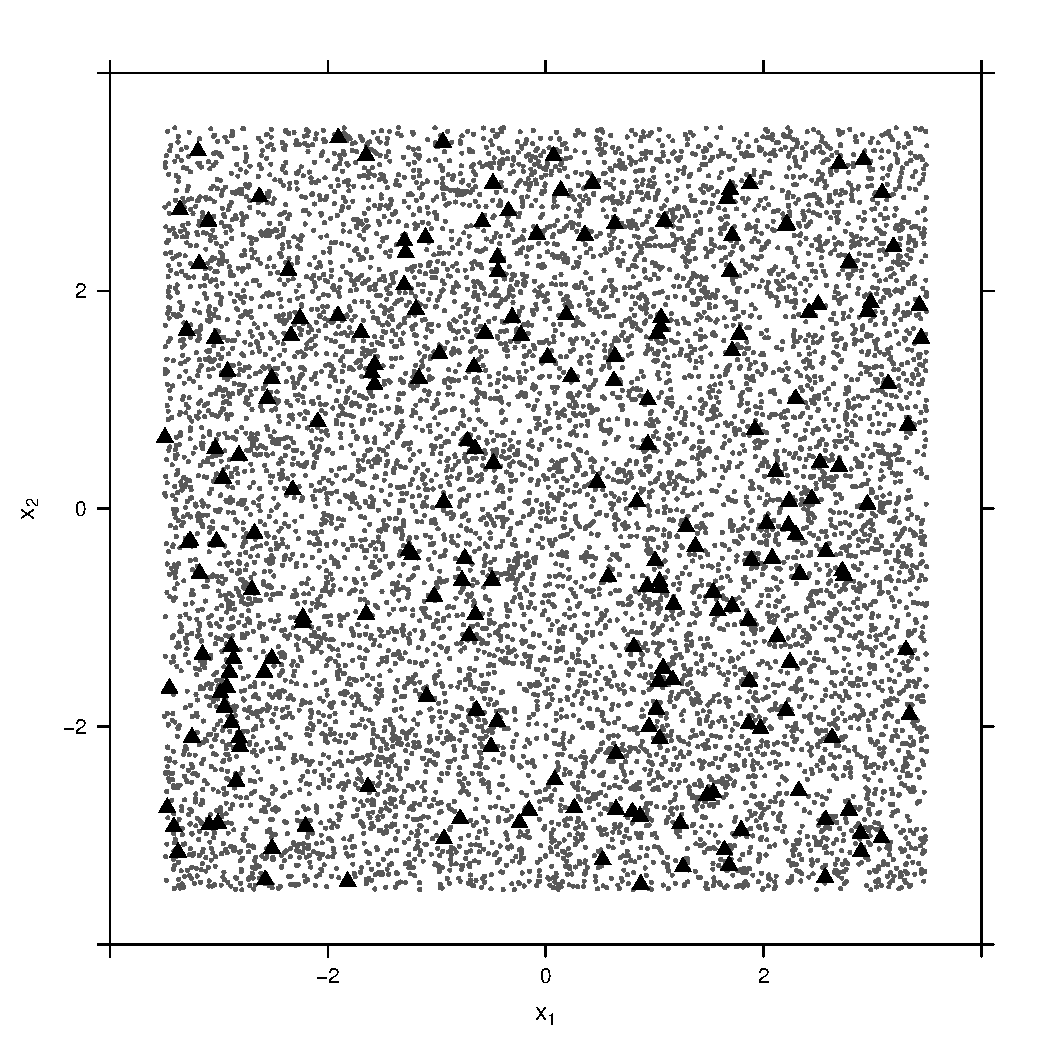
\includegraphics[width=\textwidth]{output/population_and_incidents_scatter}
    \subcaption{Population points (gray) with incidents (black)}
    \end{subfigure}%

    \caption[]{Population distribution (a), true risk function (b), and sample population with incidents (c) for uniform population of 10,000, uniform risk of factor 200}
    \label{fig:distributions:unif_200_unif}    
\end{figure}


%%
%% Tables and figures for uniform population of 10,000, uniform risk of factor 500
%%
\graphicspath{{./results/unif_500_unif/}}
\makeatletter
\def\input@path{{./results/unif_500_unif/}}
\makeatother

\begin{table}[H]
    \centering
    \tiny
    \begin{subtable}[t]{0.5\textwidth}
        \centering
        \subcaption{Means} 
        % latex table generated in R 3.4.2 by xtable 1.8-2 package
% Sat Feb 17 16:44:44 2018
\begin{tabular}{lrrr}
  \hline
 & Oracle & Silverman & CV \\ 
  \hline
MISE & 0.000053 & 0.000083 & 0.000080 \\ 
  Relative MISE & 0.002028 & 0.003195 & 0.003047 \\ 
  Normalized MISE & 0.000026 & 0.000042 & 0.000040 \\ 
  MIAE & 0.003914 & 0.004863 & 0.004653 \\ 
  Relative MIAE & 0.024227 & 0.030102 & 0.028802 \\ 
  Max Error & 0.033855 & 0.049415 & 0.045884 \\ 
  Peak bias & -0.016050 & 0.010816 & -0.002953 \\ 
  Relative Peak bias & -0.099339 & 0.066949 & -0.018278 \\ 
  Peak drift & 0.223424 & 0.357624 & 0.284159 \\ 
  Relative Peak drift & 0.031918 & 0.051089 & 0.040594 \\ 
  Centroid bias & -0.017140 & -0.000902 & -0.013918 \\ 
  Relative Centroid bias & -0.106087 & -0.005583 & -0.086149 \\ 
  Centroid drift & 0.149249 & 0.159867 & 0.152694 \\ 
  Relative Centroid drift & 0.021321 & 0.022838 & 0.021813 \\ 
   \hline
\end{tabular}

    \end{subtable}%
    \begin{subtable}[t]{0.5\textwidth}
        \centering
        \subcaption{Standard deviations} 
        % latex table generated in R 3.4.3 by xtable 1.8-2 package
% Sun Apr 15 09:09:45 2018
\begin{tabular}{lrrr}
  \toprule
 & Oracle & Silverman & CV \\ 
  \midrule
MISE & 0.000014 & 0.000014 & 0.000021 \\ 
  Relative MISE & 0.001962 & 0.002039 & 0.003010 \\ 
  Normalized MISE & 0.344229 & 0.357804 & 0.528098 \\ 
  MIAE & 0.000689 & 0.000597 & 0.000961 \\ 
  Relative MIAE & 0.008228 & 0.007121 & 0.011473 \\ 
  Normalized MIAE & 0.000003 & 0.000003 & 0.000005 \\ 
  Supremum error & 0.005321 & 0.006343 & 0.008947 \\ 
  Normalized Sup error & 0.000027 & 0.000032 & 0.000045 \\ 
  Peak bias & 0.008408 & 0.012518 & 0.015040 \\ 
  Relative Peak bias & 0.100360 & 0.149419 & 0.179526 \\ 
  Peak drift & 0.186254 & 0.253752 & 0.225627 \\ 
  Relative Peak drift & 0.026608 & 0.036250 & 0.032232 \\ 
  Centroid bias & 0.008526 & 0.013326 & 0.013412 \\ 
  Relative Centroid bias & 0.101772 & 0.159063 & 0.160095 \\ 
  Centroid drift & 0.142123 & 0.159726 & 0.144847 \\ 
  Relative Centroid drift & 0.020303 & 0.022818 & 0.020692 \\ 
   \bottomrule
\end{tabular}

    \end{subtable}

\caption[]{Error rates for uniform population of 10,000, uniform risk of factor 500}
\label{tab:mean_error_rates:unif_500_unif}
\end{table}

\begin{figure}[H]
        \centering
    \begin{subfigure}[t]{0.33\textwidth}
    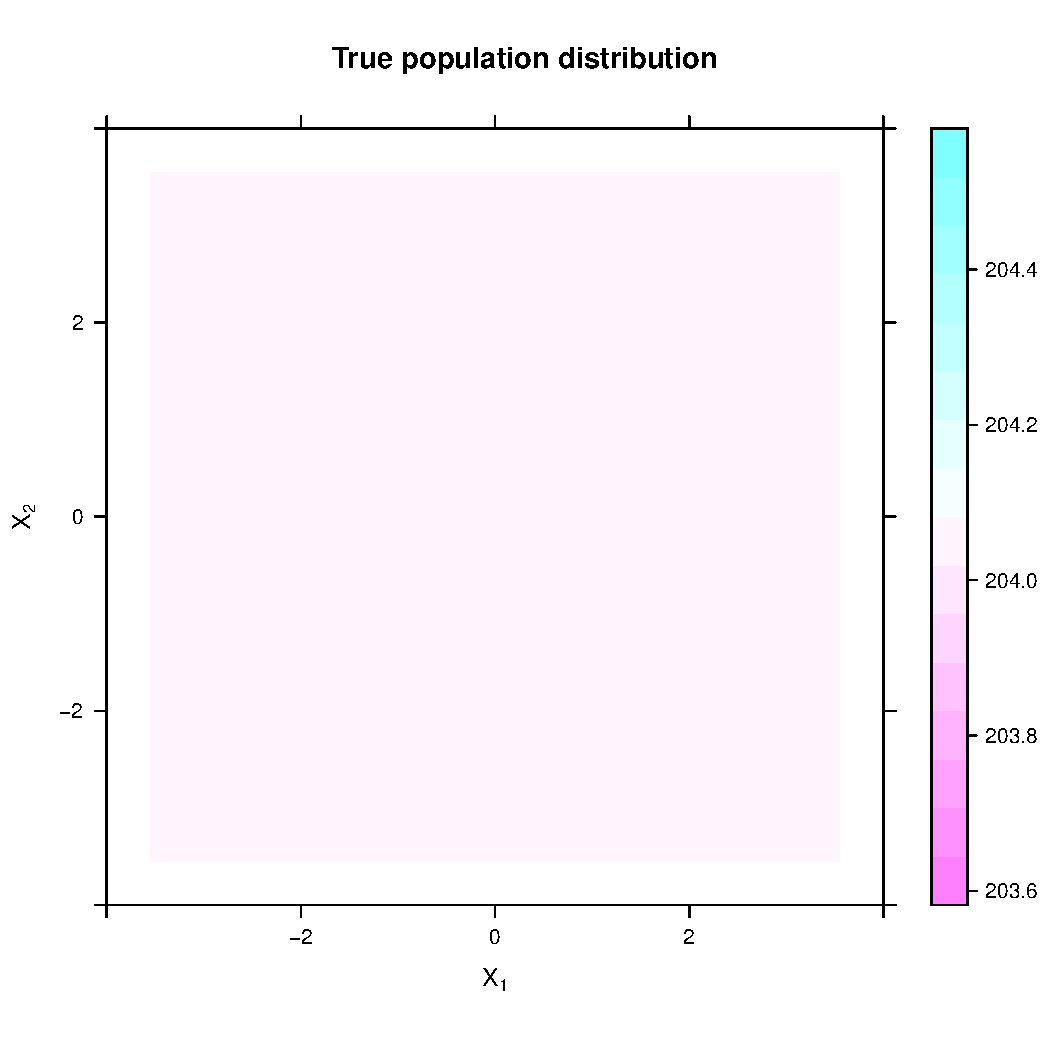
\includegraphics[width=\textwidth]{output/population-heatmap}
    \subcaption{Population distribution}
    \end{subfigure}
    \begin{subfigure}[t]{0.33\textwidth}
    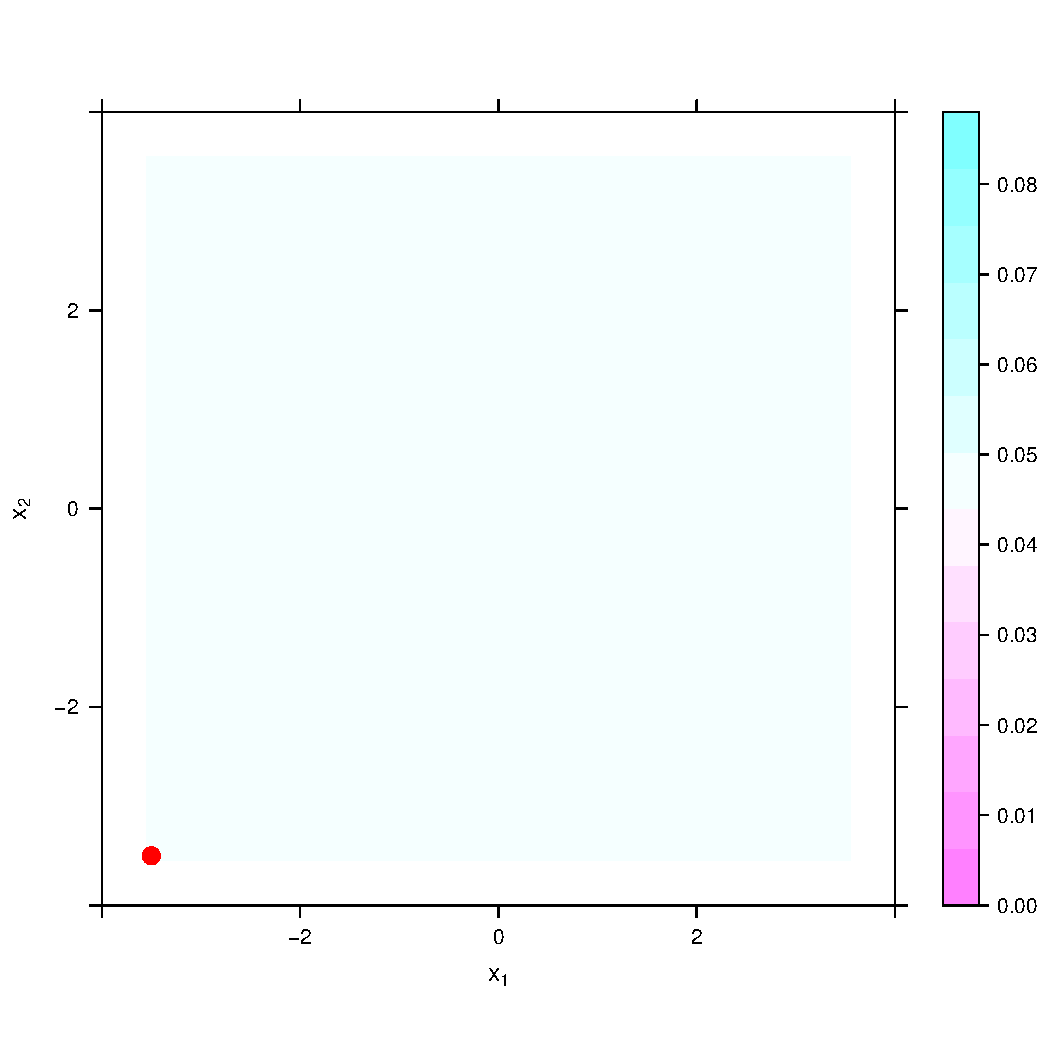
\includegraphics[width=\textwidth]{output/true_intensity_heatmap}
    \subcaption{True risk function}
    \end{subfigure}%
    \begin{subfigure}[t]{0.32\textwidth}
    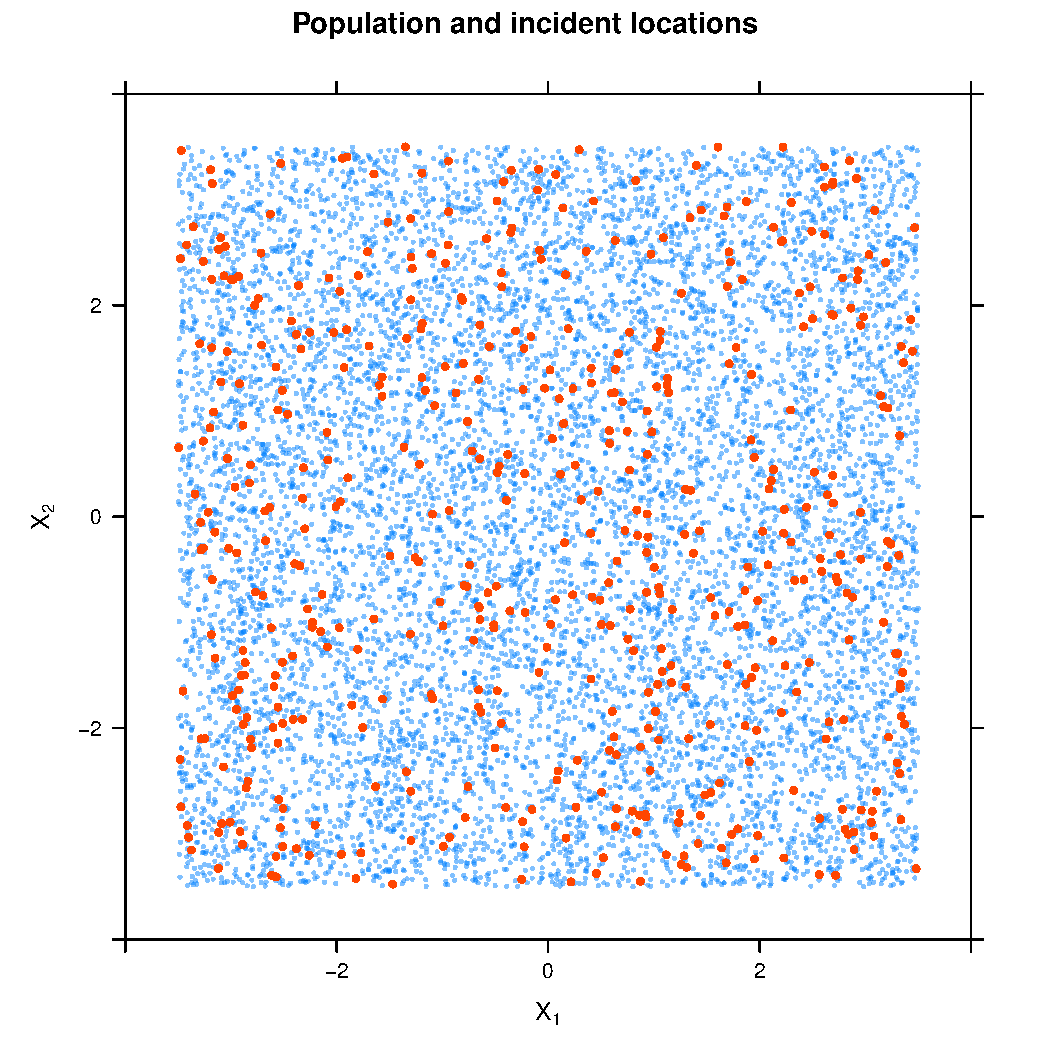
\includegraphics[width=\textwidth]{output/population_and_incidents_scatter}
    \subcaption{Population points (gray) with incidents (black)}
    \end{subfigure}%

    \caption[]{Population distribution (a), true risk function (b), and sample population with incidents (c) for uniform population of 10,000, uniform risk of factor 500}
    \label{fig:distributions:unif_500_unif}    
\end{figure}


%%
%% Tables and figures for uniform population of 10,000, uniform risk of factor 1,000
%%
\graphicspath{{./results/unif_1000_unif/}}
\makeatletter
\def\input@path{{./results/unif_1000_unif/}}
\makeatother

\begin{table}[H]
    \centering
    \tiny
    \begin{subtable}[t]{0.5\textwidth}
        \centering
        \subcaption{Means} 
        % latex table generated in R 3.4.2 by xtable 1.8-2 package
% Sat Feb 17 16:44:44 2018
\begin{tabular}{lrrr}
  \hline
 & Oracle & Silverman & CV \\ 
  \hline
MISE & 0.000053 & 0.000083 & 0.000080 \\ 
  Relative MISE & 0.002028 & 0.003195 & 0.003047 \\ 
  Normalized MISE & 0.000026 & 0.000042 & 0.000040 \\ 
  MIAE & 0.003914 & 0.004863 & 0.004653 \\ 
  Relative MIAE & 0.024227 & 0.030102 & 0.028802 \\ 
  Max Error & 0.033855 & 0.049415 & 0.045884 \\ 
  Peak bias & -0.016050 & 0.010816 & -0.002953 \\ 
  Relative Peak bias & -0.099339 & 0.066949 & -0.018278 \\ 
  Peak drift & 0.223424 & 0.357624 & 0.284159 \\ 
  Relative Peak drift & 0.031918 & 0.051089 & 0.040594 \\ 
  Centroid bias & -0.017140 & -0.000902 & -0.013918 \\ 
  Relative Centroid bias & -0.106087 & -0.005583 & -0.086149 \\ 
  Centroid drift & 0.149249 & 0.159867 & 0.152694 \\ 
  Relative Centroid drift & 0.021321 & 0.022838 & 0.021813 \\ 
   \hline
\end{tabular}

    \end{subtable}%
    \begin{subtable}[t]{0.5\textwidth}
        \centering
        \subcaption{Standard deviations} 
        % latex table generated in R 3.4.3 by xtable 1.8-2 package
% Sun Apr 15 09:09:45 2018
\begin{tabular}{lrrr}
  \toprule
 & Oracle & Silverman & CV \\ 
  \midrule
MISE & 0.000014 & 0.000014 & 0.000021 \\ 
  Relative MISE & 0.001962 & 0.002039 & 0.003010 \\ 
  Normalized MISE & 0.344229 & 0.357804 & 0.528098 \\ 
  MIAE & 0.000689 & 0.000597 & 0.000961 \\ 
  Relative MIAE & 0.008228 & 0.007121 & 0.011473 \\ 
  Normalized MIAE & 0.000003 & 0.000003 & 0.000005 \\ 
  Supremum error & 0.005321 & 0.006343 & 0.008947 \\ 
  Normalized Sup error & 0.000027 & 0.000032 & 0.000045 \\ 
  Peak bias & 0.008408 & 0.012518 & 0.015040 \\ 
  Relative Peak bias & 0.100360 & 0.149419 & 0.179526 \\ 
  Peak drift & 0.186254 & 0.253752 & 0.225627 \\ 
  Relative Peak drift & 0.026608 & 0.036250 & 0.032232 \\ 
  Centroid bias & 0.008526 & 0.013326 & 0.013412 \\ 
  Relative Centroid bias & 0.101772 & 0.159063 & 0.160095 \\ 
  Centroid drift & 0.142123 & 0.159726 & 0.144847 \\ 
  Relative Centroid drift & 0.020303 & 0.022818 & 0.020692 \\ 
   \bottomrule
\end{tabular}

    \end{subtable}

\caption[]{Error rates for uniform population of 10,000, uniform risk of factor 1,000}
\label{tab:mean_error_rates:unif_1000_unif}
\end{table}

\begin{figure}[H]
        \centering
    \begin{subfigure}[t]{0.33\textwidth}
    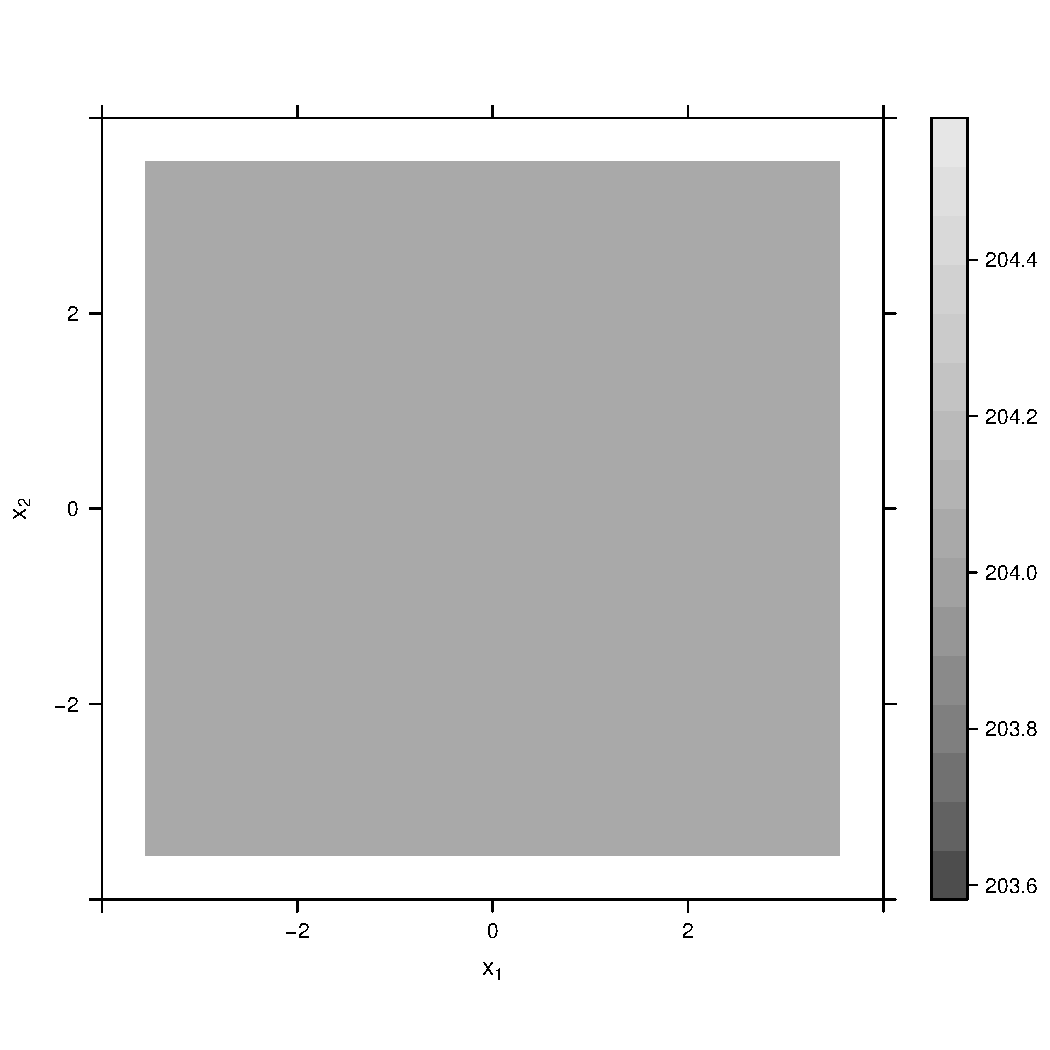
\includegraphics[width=\textwidth]{output/population-heatmap}
    \subcaption{Population distribution}
    \end{subfigure}
    \begin{subfigure}[t]{0.33\textwidth}
    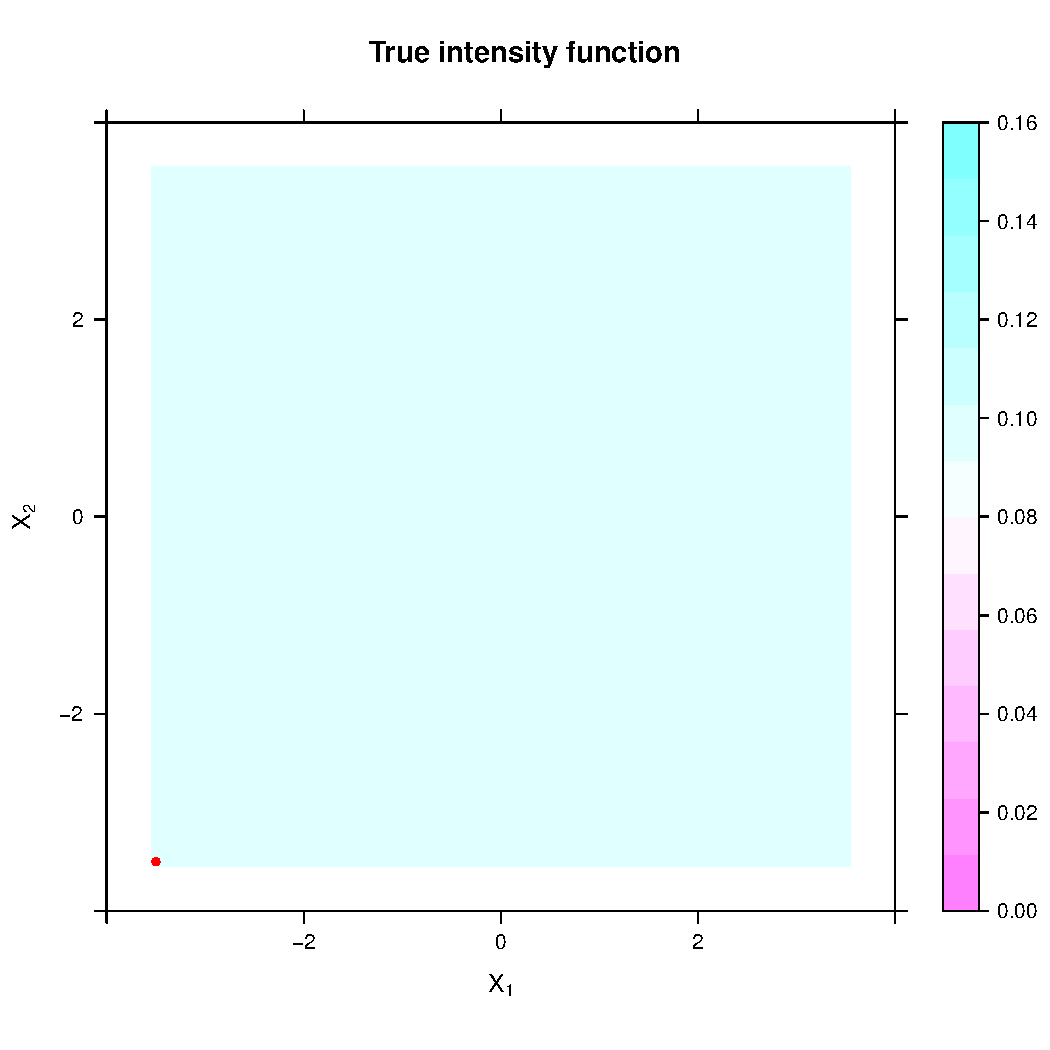
\includegraphics[width=\textwidth]{output/true_intensity_heatmap}
    \subcaption{True risk function}
    \end{subfigure}%
    \begin{subfigure}[t]{0.32\textwidth}
    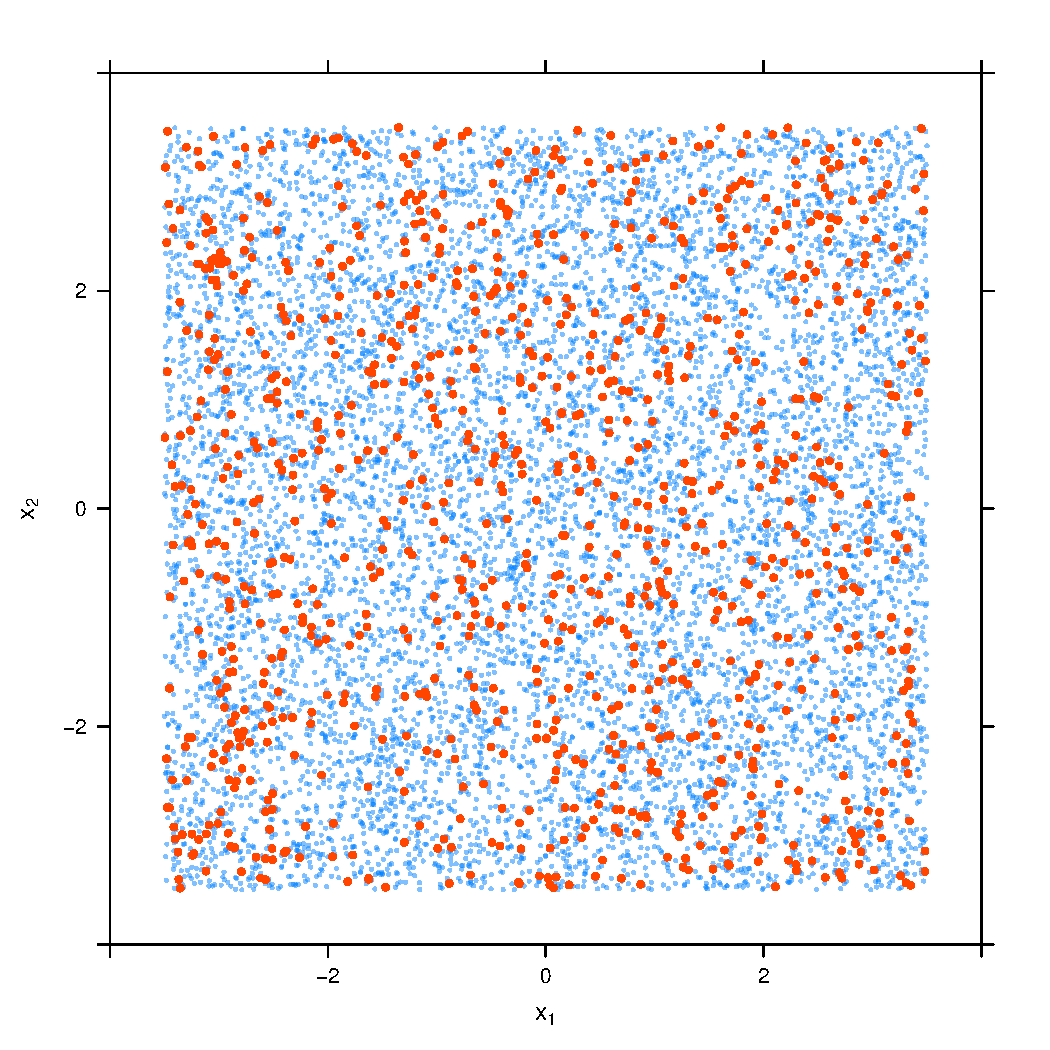
\includegraphics[width=\textwidth]{output/population_and_incidents_scatter}
    \subcaption{Population points (gray) with incidents (black)}
    \end{subfigure}%

    \caption[]{Population distribution (a), true risk function (b), and sample population with incidents (c) for uniform population of 10,000, uniform risk of factor 1,000}
    \label{fig:distributions:unif_1000_unif}    
\end{figure}

%%
%% Section containing single-peak risk with decay rate 0.7 on uniform population
%%
\section{Single-peak risk with decay rate 0.7 on a uniform population}
\label{sec:app:results_unif_0.7_1h}

%%
%% Tables and figures for uniform population of 10,000, single-peak risk of decay rate 0.7, factor 50
%%
\graphicspath{{./results/unif_50_0.7_1h/}}
\makeatletter
\def\input@path{{./results/unif_50_0.7_1h/}}
\makeatother

\begin{table}[H]
        \centering
    \tiny
    \begin{subtable}[t]{0.5\textwidth}
        \centering
        \subcaption{Means} 
        % latex table generated in R 3.4.2 by xtable 1.8-2 package
% Sat Feb 17 16:44:44 2018
\begin{tabular}{lrrr}
  \hline
 & Oracle & Silverman & CV \\ 
  \hline
MISE & 0.000053 & 0.000083 & 0.000080 \\ 
  Relative MISE & 0.002028 & 0.003195 & 0.003047 \\ 
  Normalized MISE & 0.000026 & 0.000042 & 0.000040 \\ 
  MIAE & 0.003914 & 0.004863 & 0.004653 \\ 
  Relative MIAE & 0.024227 & 0.030102 & 0.028802 \\ 
  Max Error & 0.033855 & 0.049415 & 0.045884 \\ 
  Peak bias & -0.016050 & 0.010816 & -0.002953 \\ 
  Relative Peak bias & -0.099339 & 0.066949 & -0.018278 \\ 
  Peak drift & 0.223424 & 0.357624 & 0.284159 \\ 
  Relative Peak drift & 0.031918 & 0.051089 & 0.040594 \\ 
  Centroid bias & -0.017140 & -0.000902 & -0.013918 \\ 
  Relative Centroid bias & -0.106087 & -0.005583 & -0.086149 \\ 
  Centroid drift & 0.149249 & 0.159867 & 0.152694 \\ 
  Relative Centroid drift & 0.021321 & 0.022838 & 0.021813 \\ 
   \hline
\end{tabular}

    \end{subtable}%
    \begin{subtable}[t]{0.5\textwidth}
        \centering
        \subcaption{Standard deviations} 
        % latex table generated in R 3.4.3 by xtable 1.8-2 package
% Sun Apr 15 09:09:45 2018
\begin{tabular}{lrrr}
  \toprule
 & Oracle & Silverman & CV \\ 
  \midrule
MISE & 0.000014 & 0.000014 & 0.000021 \\ 
  Relative MISE & 0.001962 & 0.002039 & 0.003010 \\ 
  Normalized MISE & 0.344229 & 0.357804 & 0.528098 \\ 
  MIAE & 0.000689 & 0.000597 & 0.000961 \\ 
  Relative MIAE & 0.008228 & 0.007121 & 0.011473 \\ 
  Normalized MIAE & 0.000003 & 0.000003 & 0.000005 \\ 
  Supremum error & 0.005321 & 0.006343 & 0.008947 \\ 
  Normalized Sup error & 0.000027 & 0.000032 & 0.000045 \\ 
  Peak bias & 0.008408 & 0.012518 & 0.015040 \\ 
  Relative Peak bias & 0.100360 & 0.149419 & 0.179526 \\ 
  Peak drift & 0.186254 & 0.253752 & 0.225627 \\ 
  Relative Peak drift & 0.026608 & 0.036250 & 0.032232 \\ 
  Centroid bias & 0.008526 & 0.013326 & 0.013412 \\ 
  Relative Centroid bias & 0.101772 & 0.159063 & 0.160095 \\ 
  Centroid drift & 0.142123 & 0.159726 & 0.144847 \\ 
  Relative Centroid drift & 0.020303 & 0.022818 & 0.020692 \\ 
   \bottomrule
\end{tabular}

    \end{subtable}

    \caption[]{Error rates for uniform population of 10,000, single-peak risk of decay rate 0.7 and factor 50}
    \label{tab:mean_error_rates:unif_50_0.7_1h}
\end{table}

\begin{figure}[H]
        \centering
    \begin{subfigure}[t]{0.33\textwidth}
    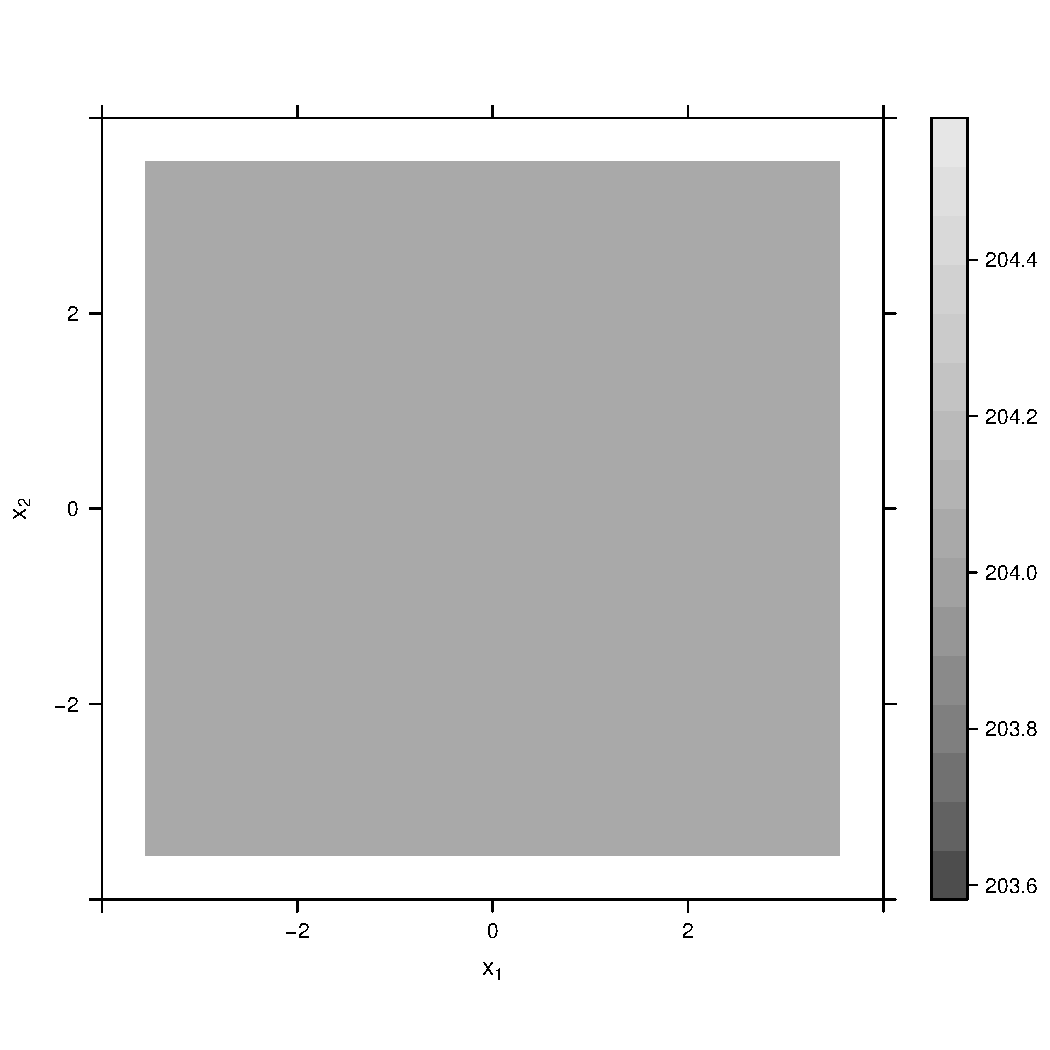
\includegraphics[width=\textwidth]{output/population-heatmap}
    \subcaption{Population distribution}
    \end{subfigure}
    \begin{subfigure}[t]{0.33\textwidth}
    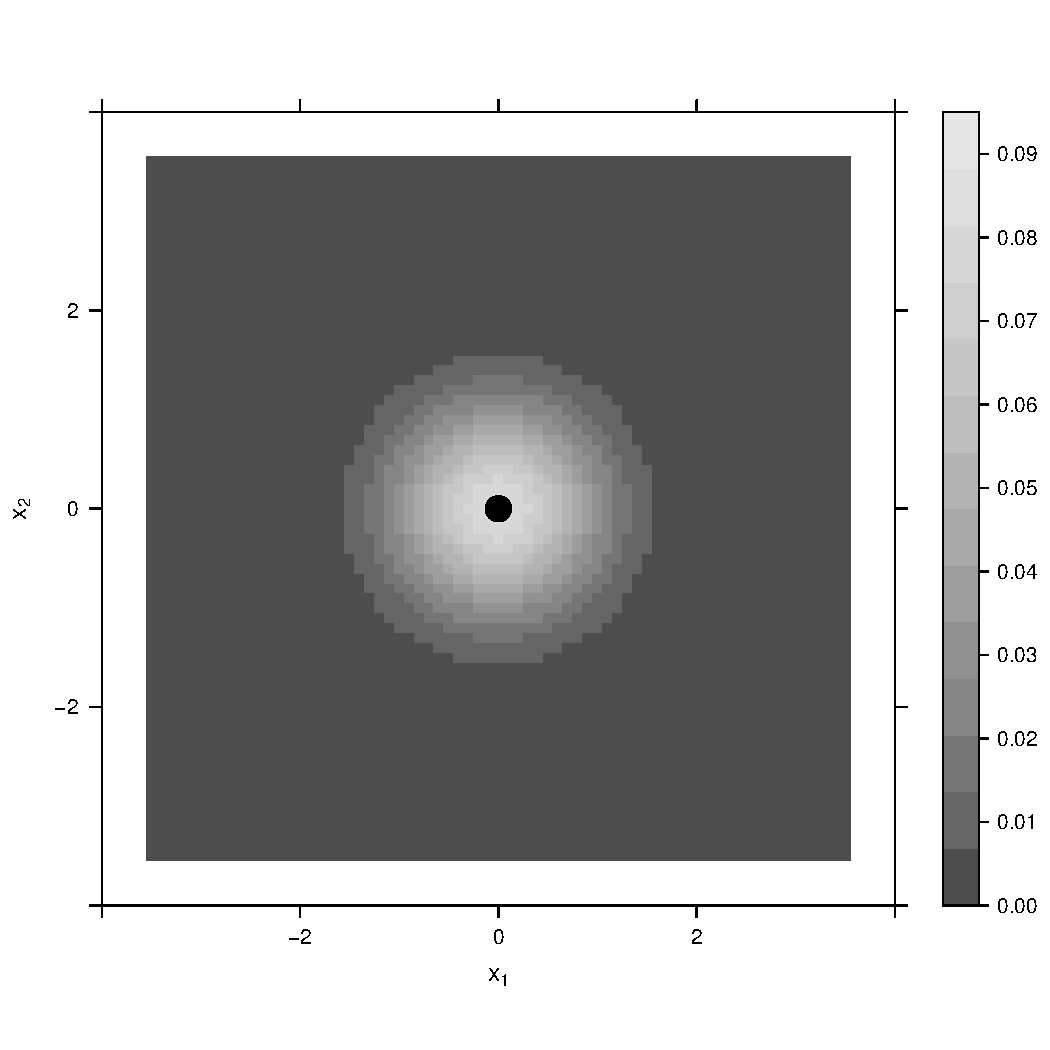
\includegraphics[width=\textwidth]{output/true_intensity_heatmap}
    \subcaption{True risk function}
    \end{subfigure}%
    \begin{subfigure}[t]{0.32\textwidth}
    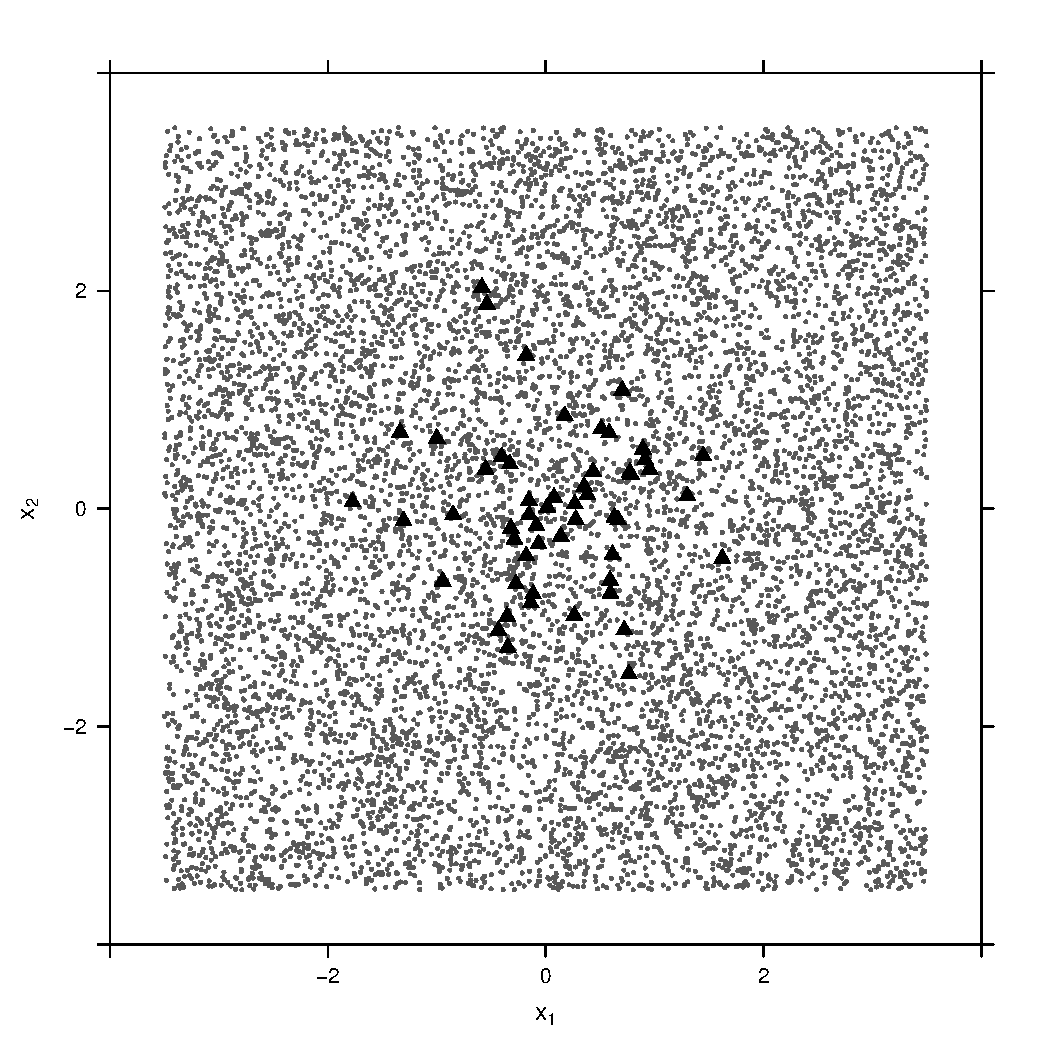
\includegraphics[width=\textwidth]{output/population_and_incidents_scatter}
    \subcaption{Population points (gray) with incidents (black)}
    \end{subfigure}%

    \caption[]{Population distribution (a), true risk function (b), and sample population with incidents (c) for uniform population of 10,000, single-peak risk of decay rate 0.7 and factor 50}
    \label{fig:distributions:unif_50_0.7_1h}    
\end{figure}


%%
%% Tables and figures for uniform population of 10,000, single-peak risk of decay rate 0.7, factor 100
%%
\graphicspath{{./results/unif_100_0.7_1h/}}
\makeatletter
\def\input@path{{./results/unif_100_0.7_1h/}}
\makeatother

\begin{table}[H]
    \centering
    \tiny
    \begin{subtable}[t]{0.5\textwidth}
        \centering
        \subcaption{Means} 
        % latex table generated in R 3.4.2 by xtable 1.8-2 package
% Sat Feb 17 16:44:44 2018
\begin{tabular}{lrrr}
  \hline
 & Oracle & Silverman & CV \\ 
  \hline
MISE & 0.000053 & 0.000083 & 0.000080 \\ 
  Relative MISE & 0.002028 & 0.003195 & 0.003047 \\ 
  Normalized MISE & 0.000026 & 0.000042 & 0.000040 \\ 
  MIAE & 0.003914 & 0.004863 & 0.004653 \\ 
  Relative MIAE & 0.024227 & 0.030102 & 0.028802 \\ 
  Max Error & 0.033855 & 0.049415 & 0.045884 \\ 
  Peak bias & -0.016050 & 0.010816 & -0.002953 \\ 
  Relative Peak bias & -0.099339 & 0.066949 & -0.018278 \\ 
  Peak drift & 0.223424 & 0.357624 & 0.284159 \\ 
  Relative Peak drift & 0.031918 & 0.051089 & 0.040594 \\ 
  Centroid bias & -0.017140 & -0.000902 & -0.013918 \\ 
  Relative Centroid bias & -0.106087 & -0.005583 & -0.086149 \\ 
  Centroid drift & 0.149249 & 0.159867 & 0.152694 \\ 
  Relative Centroid drift & 0.021321 & 0.022838 & 0.021813 \\ 
   \hline
\end{tabular}

    \end{subtable}%
    \begin{subtable}[t]{0.5\textwidth}
        \centering
        \subcaption{Standard deviations} 
        % latex table generated in R 3.4.3 by xtable 1.8-2 package
% Sun Apr 15 09:09:45 2018
\begin{tabular}{lrrr}
  \toprule
 & Oracle & Silverman & CV \\ 
  \midrule
MISE & 0.000014 & 0.000014 & 0.000021 \\ 
  Relative MISE & 0.001962 & 0.002039 & 0.003010 \\ 
  Normalized MISE & 0.344229 & 0.357804 & 0.528098 \\ 
  MIAE & 0.000689 & 0.000597 & 0.000961 \\ 
  Relative MIAE & 0.008228 & 0.007121 & 0.011473 \\ 
  Normalized MIAE & 0.000003 & 0.000003 & 0.000005 \\ 
  Supremum error & 0.005321 & 0.006343 & 0.008947 \\ 
  Normalized Sup error & 0.000027 & 0.000032 & 0.000045 \\ 
  Peak bias & 0.008408 & 0.012518 & 0.015040 \\ 
  Relative Peak bias & 0.100360 & 0.149419 & 0.179526 \\ 
  Peak drift & 0.186254 & 0.253752 & 0.225627 \\ 
  Relative Peak drift & 0.026608 & 0.036250 & 0.032232 \\ 
  Centroid bias & 0.008526 & 0.013326 & 0.013412 \\ 
  Relative Centroid bias & 0.101772 & 0.159063 & 0.160095 \\ 
  Centroid drift & 0.142123 & 0.159726 & 0.144847 \\ 
  Relative Centroid drift & 0.020303 & 0.022818 & 0.020692 \\ 
   \bottomrule
\end{tabular}

    \end{subtable}

\caption[]{Error rates for uniform population of 10,000, single-peak risk of decay rate 0.7 and factor 100}
\label{tab:mean_error_rates:unif_100_0.7_1h}
\end{table}

\begin{figure}[H]
        \centering
    \begin{subfigure}[t]{0.33\textwidth}
    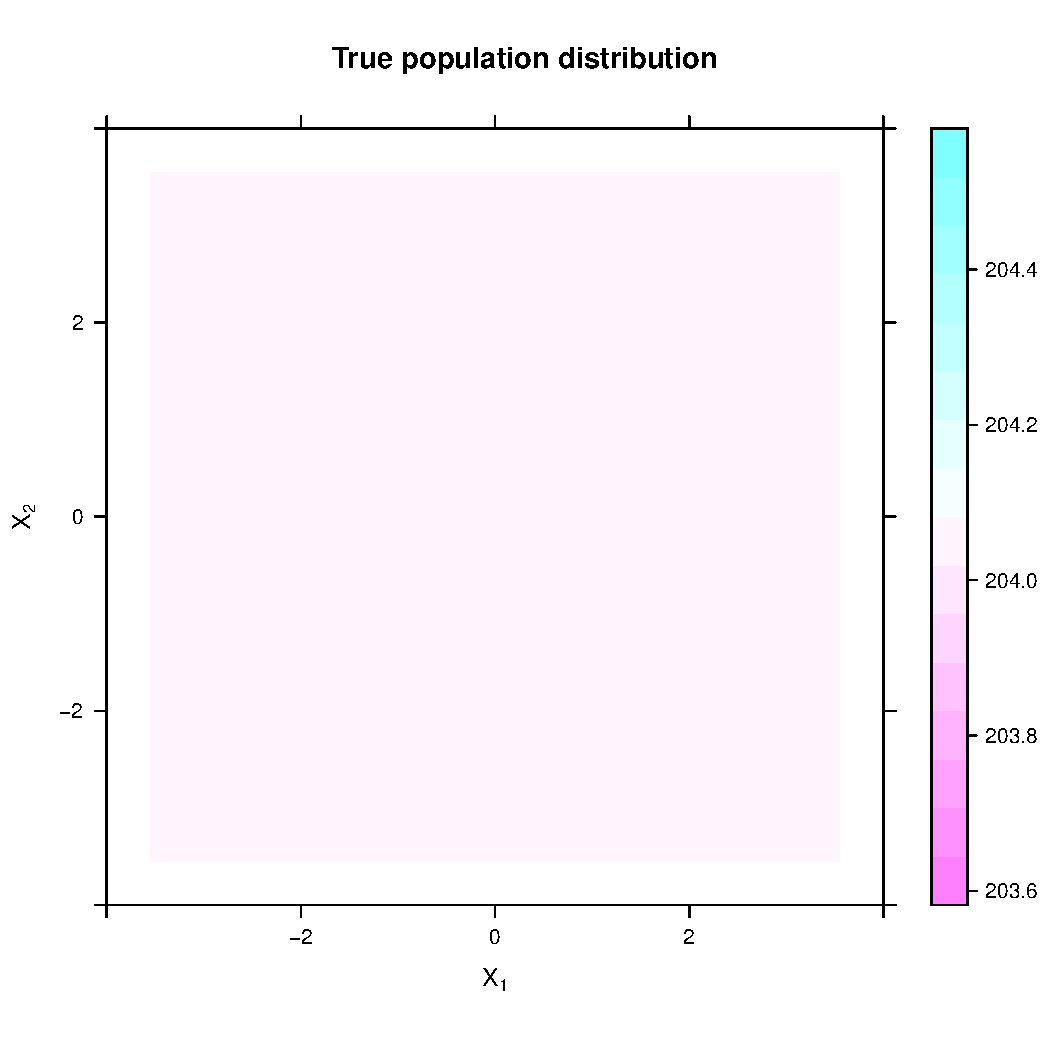
\includegraphics[width=\textwidth]{output/population-heatmap}
    \subcaption{Population distribution}
    \end{subfigure}
    \begin{subfigure}[t]{0.33\textwidth}
    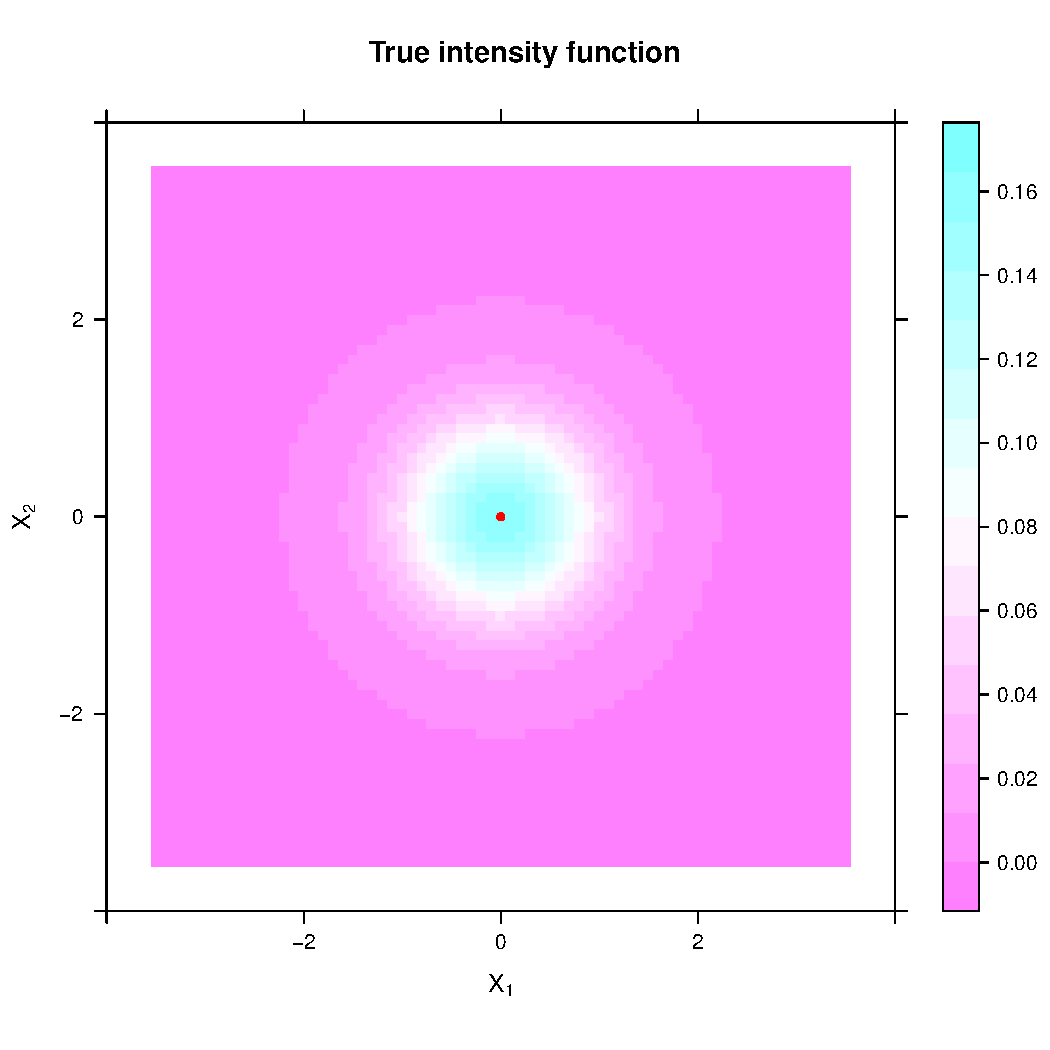
\includegraphics[width=\textwidth]{output/true_intensity_heatmap}
    \subcaption{True risk function}
    \end{subfigure}%
    \begin{subfigure}[t]{0.32\textwidth}
    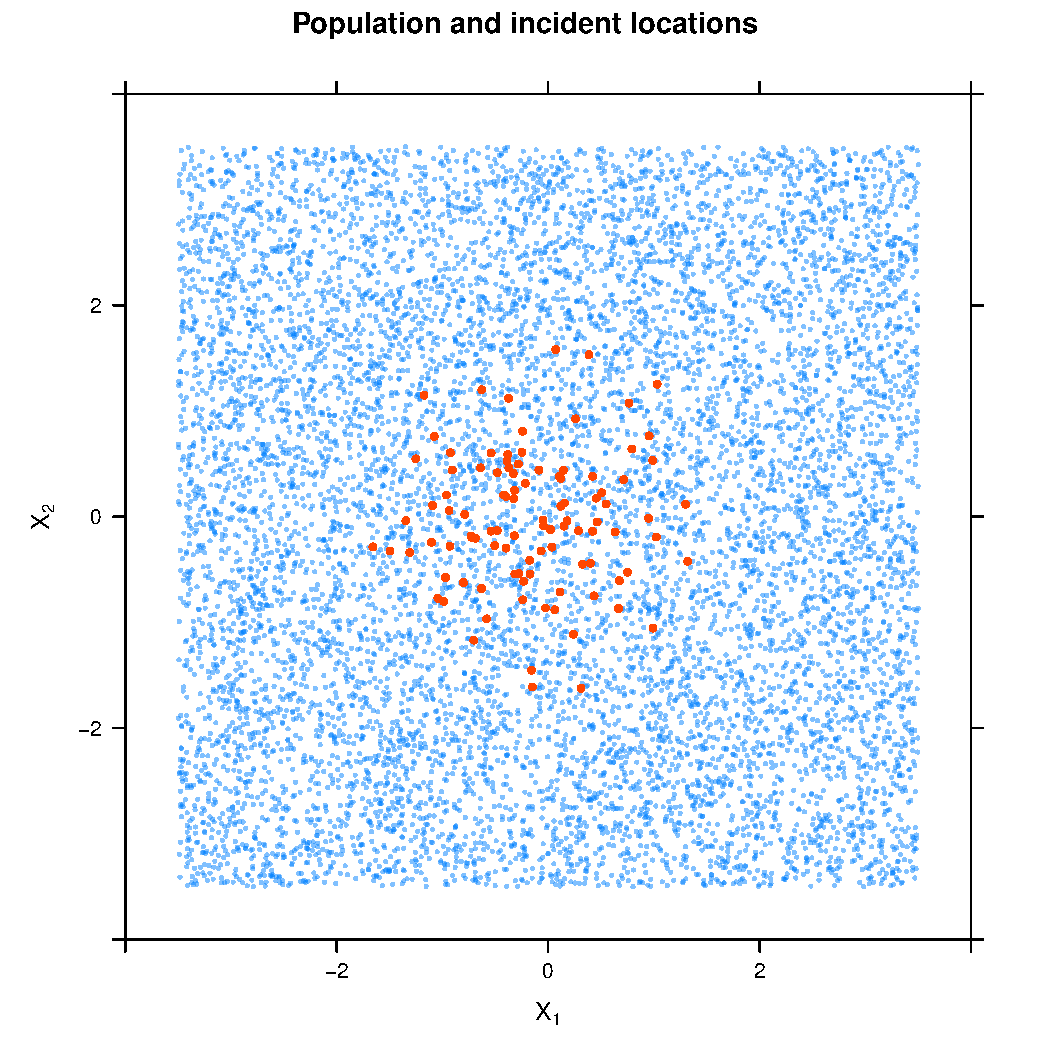
\includegraphics[width=\textwidth]{output/population_and_incidents_scatter}
    \subcaption{Population points (gray) with incidents (black)}
    \end{subfigure}%

    \caption[]{Population distribution (a), true risk function (b), and sample population with incidents (c) for uniform population of 10,000, single-peak risk of decay rate 0.7 and factor 100}
    \label{fig:distributions:unif_100_0.7_1h}    
\end{figure}


%%
%% Tables and figures for uniform population of 10,000, single-peak risk of decay rate 0.7, factor 200
%%
\graphicspath{{./results/unif_200_0.7_1h/}}
\makeatletter
\def\input@path{{./results/unif_200_0.7_1h/}}
\makeatother

\begin{table}[H]
    \centering
    \tiny
    \begin{subtable}[t]{0.5\textwidth}
        \centering
        \subcaption{Means} 
        % latex table generated in R 3.4.2 by xtable 1.8-2 package
% Sat Feb 17 16:44:44 2018
\begin{tabular}{lrrr}
  \hline
 & Oracle & Silverman & CV \\ 
  \hline
MISE & 0.000053 & 0.000083 & 0.000080 \\ 
  Relative MISE & 0.002028 & 0.003195 & 0.003047 \\ 
  Normalized MISE & 0.000026 & 0.000042 & 0.000040 \\ 
  MIAE & 0.003914 & 0.004863 & 0.004653 \\ 
  Relative MIAE & 0.024227 & 0.030102 & 0.028802 \\ 
  Max Error & 0.033855 & 0.049415 & 0.045884 \\ 
  Peak bias & -0.016050 & 0.010816 & -0.002953 \\ 
  Relative Peak bias & -0.099339 & 0.066949 & -0.018278 \\ 
  Peak drift & 0.223424 & 0.357624 & 0.284159 \\ 
  Relative Peak drift & 0.031918 & 0.051089 & 0.040594 \\ 
  Centroid bias & -0.017140 & -0.000902 & -0.013918 \\ 
  Relative Centroid bias & -0.106087 & -0.005583 & -0.086149 \\ 
  Centroid drift & 0.149249 & 0.159867 & 0.152694 \\ 
  Relative Centroid drift & 0.021321 & 0.022838 & 0.021813 \\ 
   \hline
\end{tabular}

    \end{subtable}%
    \begin{subtable}[t]{0.5\textwidth}
        \centering
        \subcaption{Standard deviations} 
        % latex table generated in R 3.4.3 by xtable 1.8-2 package
% Sun Apr 15 09:09:45 2018
\begin{tabular}{lrrr}
  \toprule
 & Oracle & Silverman & CV \\ 
  \midrule
MISE & 0.000014 & 0.000014 & 0.000021 \\ 
  Relative MISE & 0.001962 & 0.002039 & 0.003010 \\ 
  Normalized MISE & 0.344229 & 0.357804 & 0.528098 \\ 
  MIAE & 0.000689 & 0.000597 & 0.000961 \\ 
  Relative MIAE & 0.008228 & 0.007121 & 0.011473 \\ 
  Normalized MIAE & 0.000003 & 0.000003 & 0.000005 \\ 
  Supremum error & 0.005321 & 0.006343 & 0.008947 \\ 
  Normalized Sup error & 0.000027 & 0.000032 & 0.000045 \\ 
  Peak bias & 0.008408 & 0.012518 & 0.015040 \\ 
  Relative Peak bias & 0.100360 & 0.149419 & 0.179526 \\ 
  Peak drift & 0.186254 & 0.253752 & 0.225627 \\ 
  Relative Peak drift & 0.026608 & 0.036250 & 0.032232 \\ 
  Centroid bias & 0.008526 & 0.013326 & 0.013412 \\ 
  Relative Centroid bias & 0.101772 & 0.159063 & 0.160095 \\ 
  Centroid drift & 0.142123 & 0.159726 & 0.144847 \\ 
  Relative Centroid drift & 0.020303 & 0.022818 & 0.020692 \\ 
   \bottomrule
\end{tabular}

    \end{subtable}

\caption[]{Error rates for uniform population of 10,000, single-peak risk of decay rate 0.7 and factor 200}
\label{tab:mean_error_rates:unif_200_0.7_1h}
\end{table}

\begin{figure}[H]
        \centering
    \begin{subfigure}[t]{0.33\textwidth}
    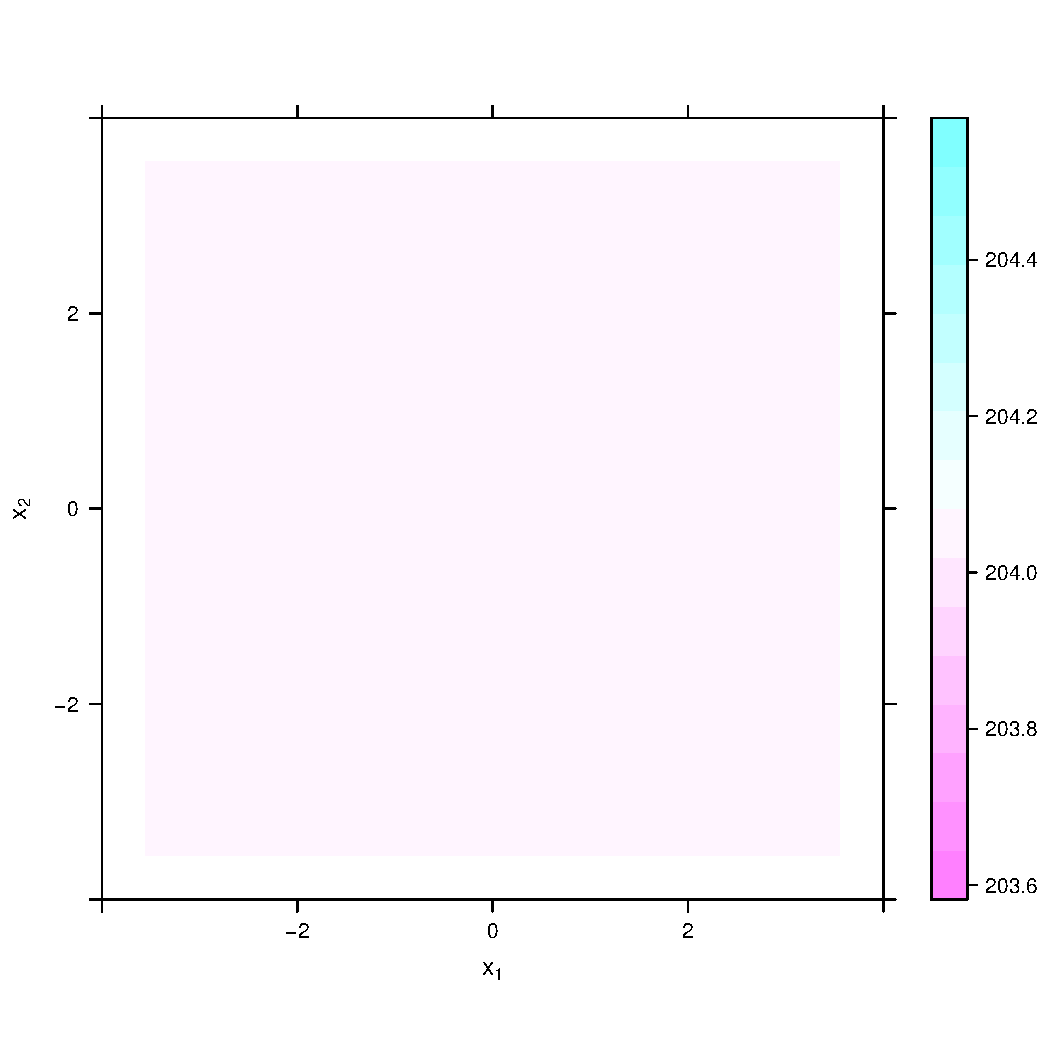
\includegraphics[width=\textwidth]{output/population-heatmap}
    \subcaption{Population distribution}
    \end{subfigure}
    \begin{subfigure}[t]{0.33\textwidth}
    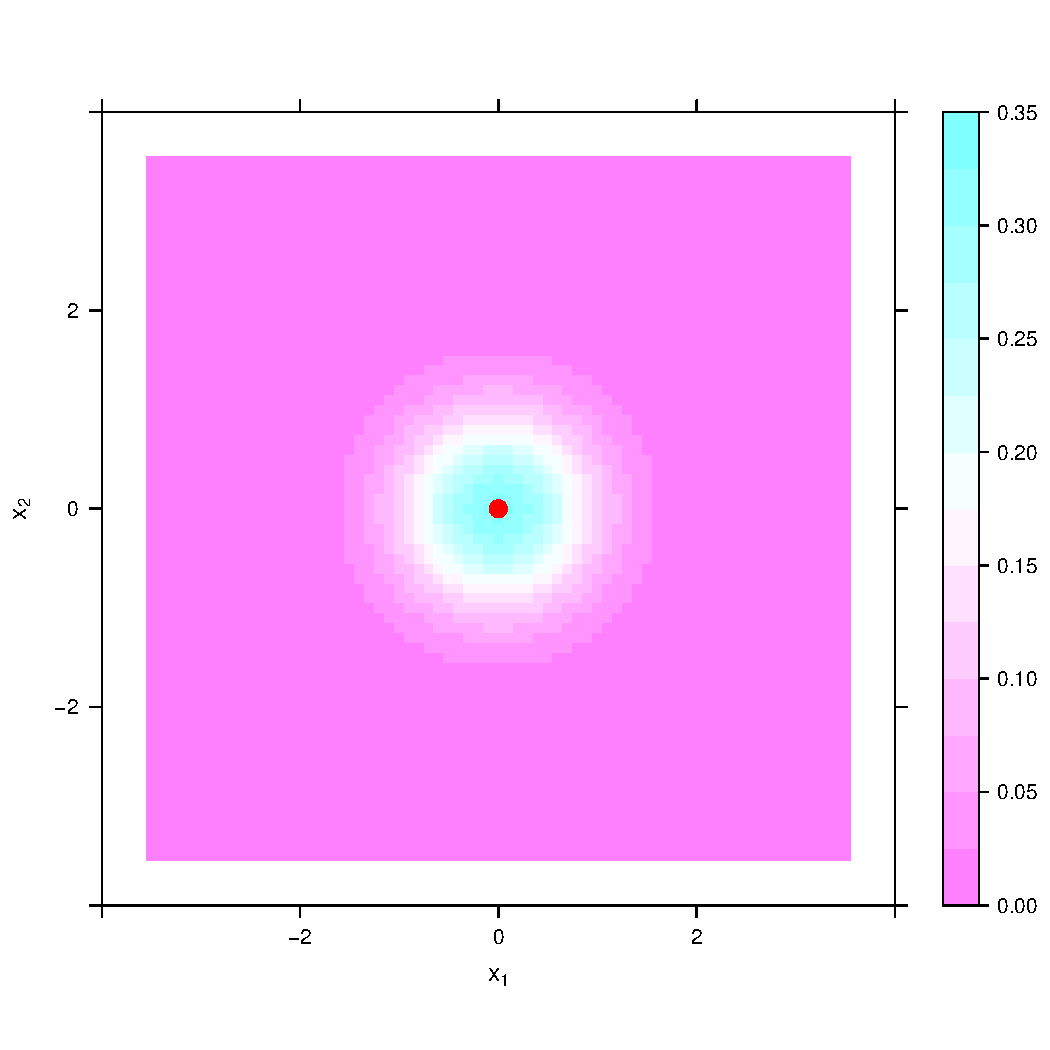
\includegraphics[width=\textwidth]{output/true_intensity_heatmap}
    \subcaption{True risk function}
    \end{subfigure}%
    \begin{subfigure}[t]{0.32\textwidth}
    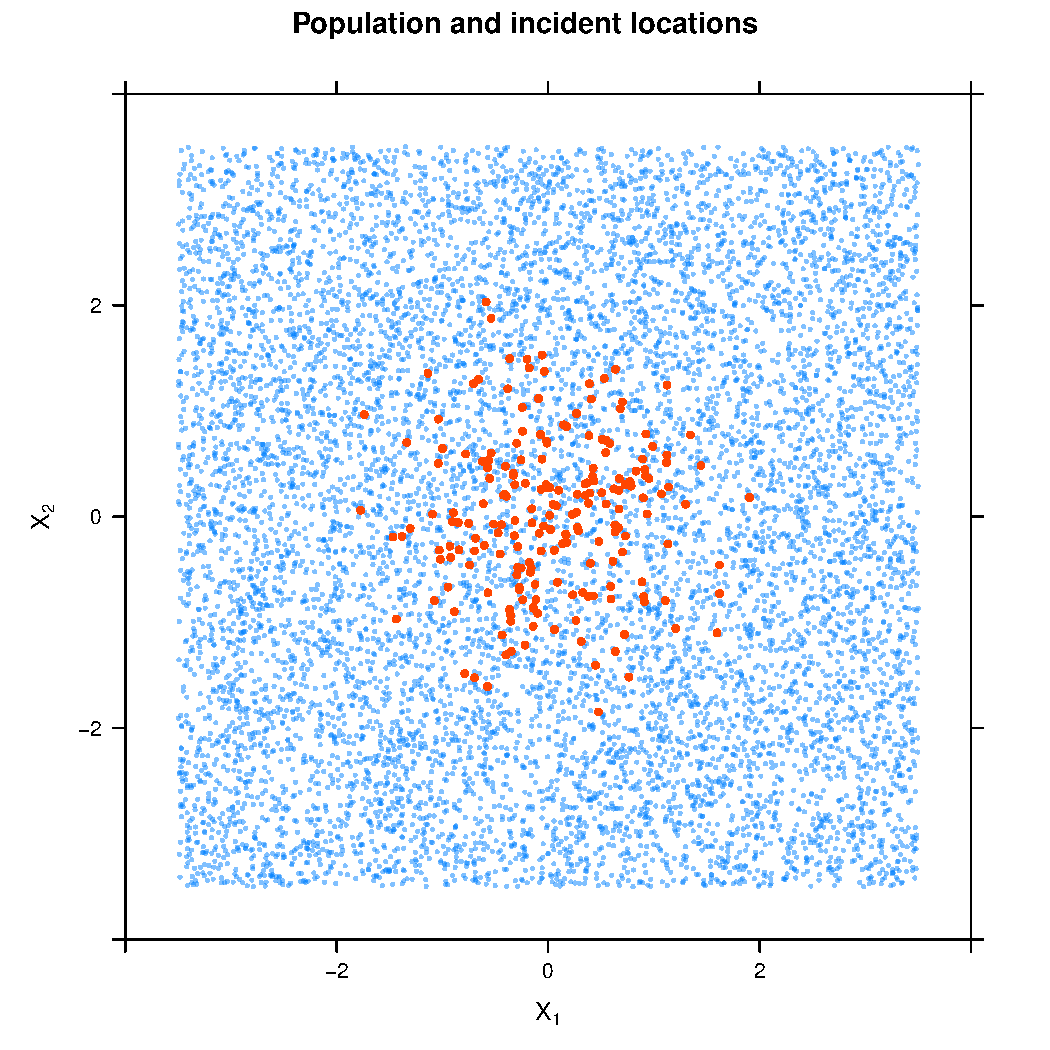
\includegraphics[width=\textwidth]{output/population_and_incidents_scatter}
    \subcaption{Population points (gray) with incidents (black)}
    \end{subfigure}%

    \caption[]{Population distribution (a), true risk function (b), and sample population with incidents (c) for uniform population of 10,000, single-peak risk of decay rate 0.7 and factor 200}
    \label{fig:distributions:unif_200_0.7_1h}    
\end{figure}


%%
%% Tables and figures for uniform population of 10,000, single-peak risk of decay rate 0.7, factor 500
%%
\graphicspath{{./results/unif_500_0.7_1h/}}
\makeatletter
\def\input@path{{./results/unif_500_0.7_1h/}}
\makeatother

\begin{table}[H]
    \centering
    \tiny
    \begin{subtable}[t]{0.5\textwidth}
        \centering
        \subcaption{Means} 
        % latex table generated in R 3.4.2 by xtable 1.8-2 package
% Sat Feb 17 16:44:44 2018
\begin{tabular}{lrrr}
  \hline
 & Oracle & Silverman & CV \\ 
  \hline
MISE & 0.000053 & 0.000083 & 0.000080 \\ 
  Relative MISE & 0.002028 & 0.003195 & 0.003047 \\ 
  Normalized MISE & 0.000026 & 0.000042 & 0.000040 \\ 
  MIAE & 0.003914 & 0.004863 & 0.004653 \\ 
  Relative MIAE & 0.024227 & 0.030102 & 0.028802 \\ 
  Max Error & 0.033855 & 0.049415 & 0.045884 \\ 
  Peak bias & -0.016050 & 0.010816 & -0.002953 \\ 
  Relative Peak bias & -0.099339 & 0.066949 & -0.018278 \\ 
  Peak drift & 0.223424 & 0.357624 & 0.284159 \\ 
  Relative Peak drift & 0.031918 & 0.051089 & 0.040594 \\ 
  Centroid bias & -0.017140 & -0.000902 & -0.013918 \\ 
  Relative Centroid bias & -0.106087 & -0.005583 & -0.086149 \\ 
  Centroid drift & 0.149249 & 0.159867 & 0.152694 \\ 
  Relative Centroid drift & 0.021321 & 0.022838 & 0.021813 \\ 
   \hline
\end{tabular}

    \end{subtable}%
    \begin{subtable}[t]{0.5\textwidth}
        \centering
        \subcaption{Standard deviations} 
        % latex table generated in R 3.4.3 by xtable 1.8-2 package
% Sun Apr 15 09:09:45 2018
\begin{tabular}{lrrr}
  \toprule
 & Oracle & Silverman & CV \\ 
  \midrule
MISE & 0.000014 & 0.000014 & 0.000021 \\ 
  Relative MISE & 0.001962 & 0.002039 & 0.003010 \\ 
  Normalized MISE & 0.344229 & 0.357804 & 0.528098 \\ 
  MIAE & 0.000689 & 0.000597 & 0.000961 \\ 
  Relative MIAE & 0.008228 & 0.007121 & 0.011473 \\ 
  Normalized MIAE & 0.000003 & 0.000003 & 0.000005 \\ 
  Supremum error & 0.005321 & 0.006343 & 0.008947 \\ 
  Normalized Sup error & 0.000027 & 0.000032 & 0.000045 \\ 
  Peak bias & 0.008408 & 0.012518 & 0.015040 \\ 
  Relative Peak bias & 0.100360 & 0.149419 & 0.179526 \\ 
  Peak drift & 0.186254 & 0.253752 & 0.225627 \\ 
  Relative Peak drift & 0.026608 & 0.036250 & 0.032232 \\ 
  Centroid bias & 0.008526 & 0.013326 & 0.013412 \\ 
  Relative Centroid bias & 0.101772 & 0.159063 & 0.160095 \\ 
  Centroid drift & 0.142123 & 0.159726 & 0.144847 \\ 
  Relative Centroid drift & 0.020303 & 0.022818 & 0.020692 \\ 
   \bottomrule
\end{tabular}

    \end{subtable}

\caption[]{Error rates for uniform population of 10,000, single-peak risk of decay rate 0.7 and factor 500}
\label{tab:mean_error_rates:unif_500_0.7_1h}
\end{table}

\begin{figure}[H]
        \centering
    \begin{subfigure}[t]{0.33\textwidth}
    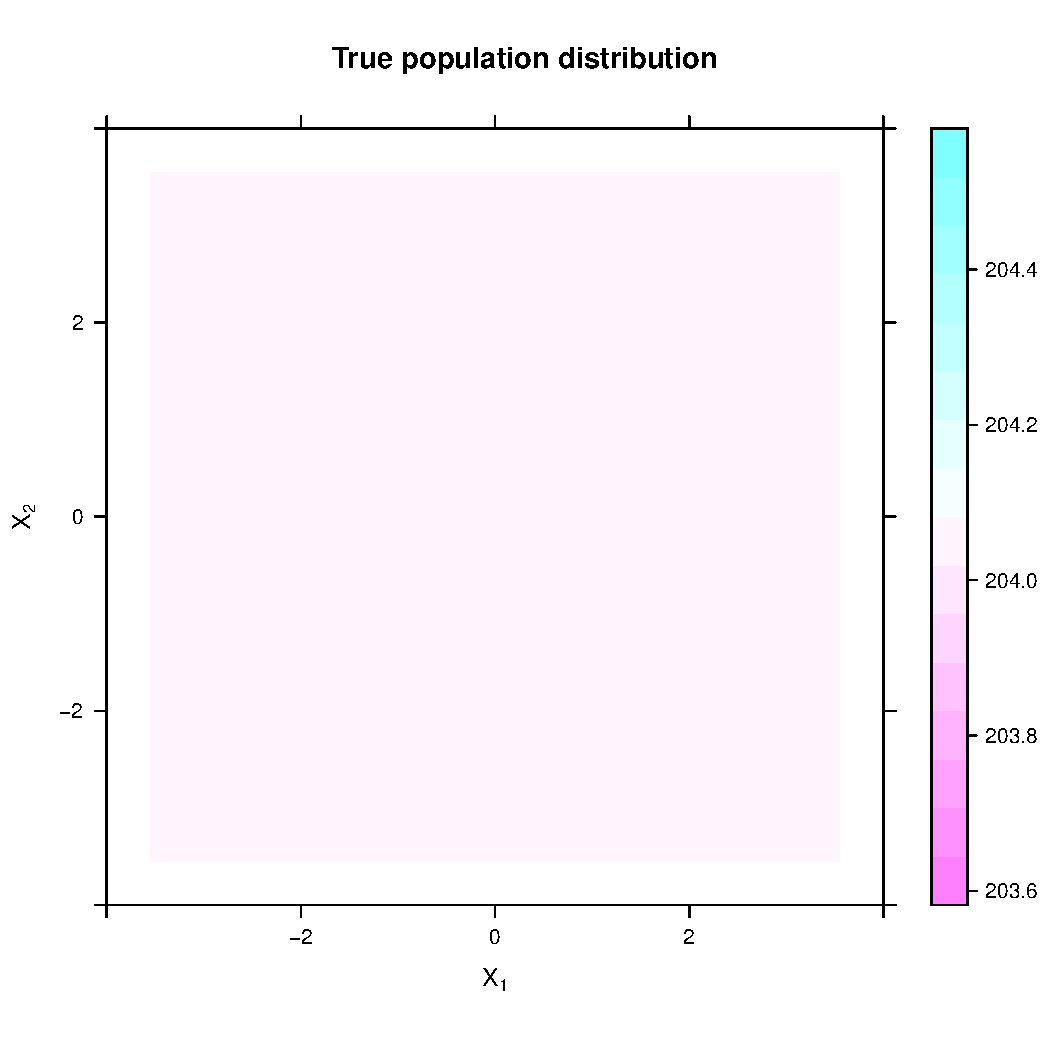
\includegraphics[width=\textwidth]{output/population-heatmap}
    \subcaption{Population distribution}
    \end{subfigure}
    \begin{subfigure}[t]{0.33\textwidth}
    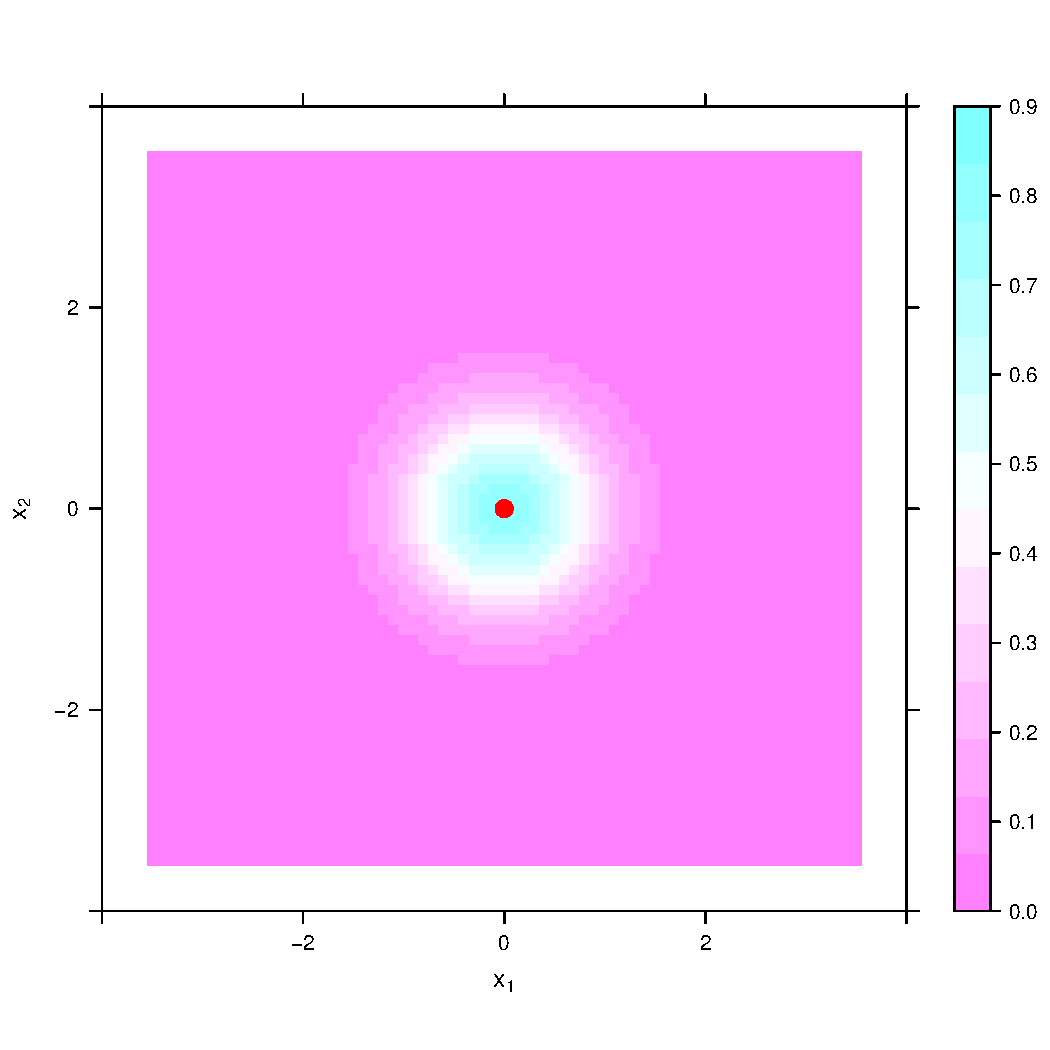
\includegraphics[width=\textwidth]{output/true_intensity_heatmap}
    \subcaption{True risk function}
    \end{subfigure}%
    \begin{subfigure}[t]{0.32\textwidth}
    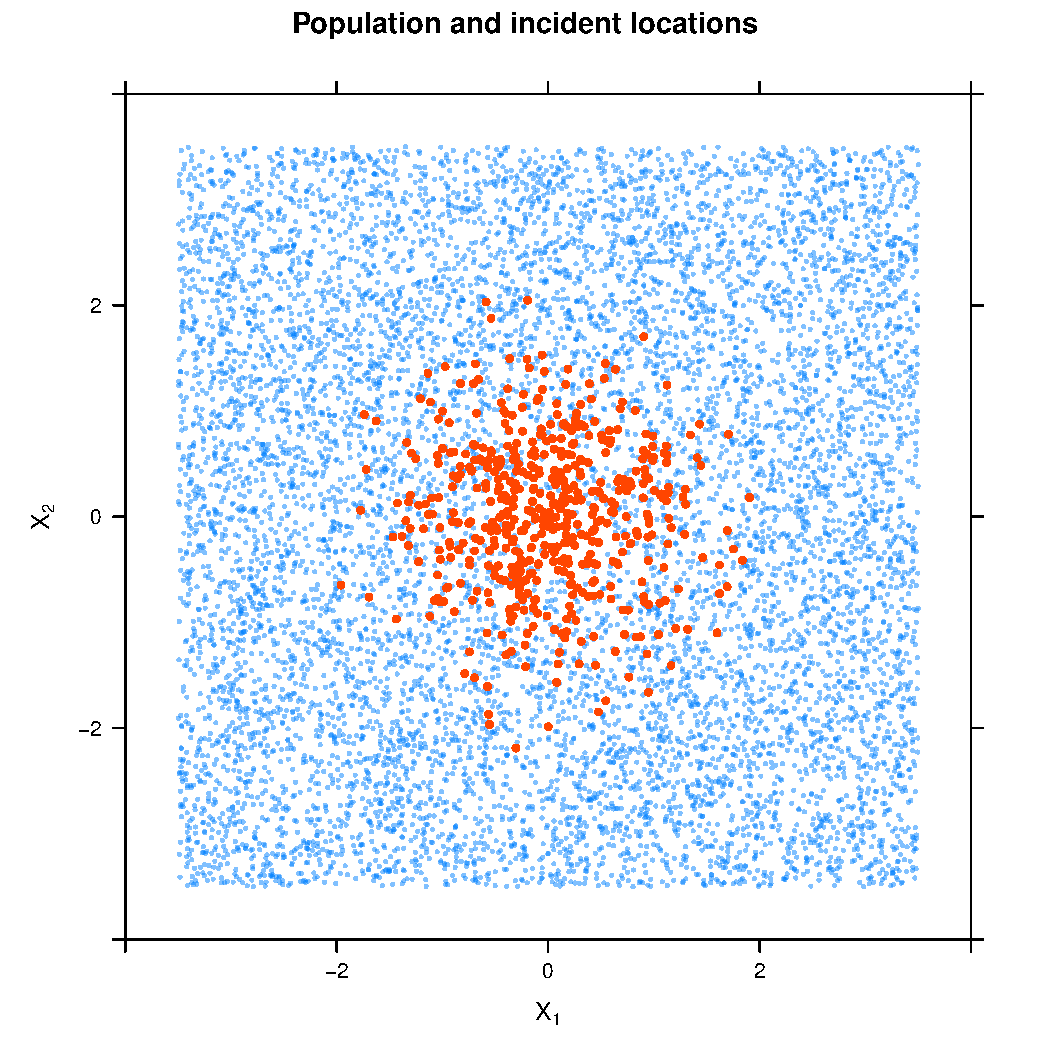
\includegraphics[width=\textwidth]{output/population_and_incidents_scatter}
    \subcaption{Population points (gray) with incidents (black)}
    \end{subfigure}%

    \caption[]{Population distribution (a), true risk function (b), and sample population with incidents (c) for uniform population of 10,000, single-peak risk of decay rate 0.7 and factor 500}
    \label{fig:distributions:unif_500_0.7_1h}    
\end{figure}


%%
%% Tables and figures for uniform population of 10,000, single-peak risk of decay rate 0.7, factor 1,000
%%
\graphicspath{{./results/unif_1000_0.7_1h/}}
\makeatletter
\def\input@path{{./results/unif_1000_0.7_1h/}}
\makeatother

\begin{table}[H]
    \centering
    \tiny
    \begin{subtable}[t]{0.5\textwidth}
        \centering
        \subcaption{Means} 
        % latex table generated in R 3.4.2 by xtable 1.8-2 package
% Sat Feb 17 16:44:44 2018
\begin{tabular}{lrrr}
  \hline
 & Oracle & Silverman & CV \\ 
  \hline
MISE & 0.000053 & 0.000083 & 0.000080 \\ 
  Relative MISE & 0.002028 & 0.003195 & 0.003047 \\ 
  Normalized MISE & 0.000026 & 0.000042 & 0.000040 \\ 
  MIAE & 0.003914 & 0.004863 & 0.004653 \\ 
  Relative MIAE & 0.024227 & 0.030102 & 0.028802 \\ 
  Max Error & 0.033855 & 0.049415 & 0.045884 \\ 
  Peak bias & -0.016050 & 0.010816 & -0.002953 \\ 
  Relative Peak bias & -0.099339 & 0.066949 & -0.018278 \\ 
  Peak drift & 0.223424 & 0.357624 & 0.284159 \\ 
  Relative Peak drift & 0.031918 & 0.051089 & 0.040594 \\ 
  Centroid bias & -0.017140 & -0.000902 & -0.013918 \\ 
  Relative Centroid bias & -0.106087 & -0.005583 & -0.086149 \\ 
  Centroid drift & 0.149249 & 0.159867 & 0.152694 \\ 
  Relative Centroid drift & 0.021321 & 0.022838 & 0.021813 \\ 
   \hline
\end{tabular}

    \end{subtable}%
    \begin{subtable}[t]{0.5\textwidth}
        \centering
        \subcaption{Standard deviations} 
        % latex table generated in R 3.4.3 by xtable 1.8-2 package
% Sun Apr 15 09:09:45 2018
\begin{tabular}{lrrr}
  \toprule
 & Oracle & Silverman & CV \\ 
  \midrule
MISE & 0.000014 & 0.000014 & 0.000021 \\ 
  Relative MISE & 0.001962 & 0.002039 & 0.003010 \\ 
  Normalized MISE & 0.344229 & 0.357804 & 0.528098 \\ 
  MIAE & 0.000689 & 0.000597 & 0.000961 \\ 
  Relative MIAE & 0.008228 & 0.007121 & 0.011473 \\ 
  Normalized MIAE & 0.000003 & 0.000003 & 0.000005 \\ 
  Supremum error & 0.005321 & 0.006343 & 0.008947 \\ 
  Normalized Sup error & 0.000027 & 0.000032 & 0.000045 \\ 
  Peak bias & 0.008408 & 0.012518 & 0.015040 \\ 
  Relative Peak bias & 0.100360 & 0.149419 & 0.179526 \\ 
  Peak drift & 0.186254 & 0.253752 & 0.225627 \\ 
  Relative Peak drift & 0.026608 & 0.036250 & 0.032232 \\ 
  Centroid bias & 0.008526 & 0.013326 & 0.013412 \\ 
  Relative Centroid bias & 0.101772 & 0.159063 & 0.160095 \\ 
  Centroid drift & 0.142123 & 0.159726 & 0.144847 \\ 
  Relative Centroid drift & 0.020303 & 0.022818 & 0.020692 \\ 
   \bottomrule
\end{tabular}

    \end{subtable}

\caption[]{Error rates for uniform population of 10,000, single-peak risk of decay rate 0.7 and factor 1,000}
\label{tab:mean_error_rates:unif_1000_0.7_1h}
\end{table}

\begin{figure}[H]
        \centering
    \begin{subfigure}[t]{0.33\textwidth}
    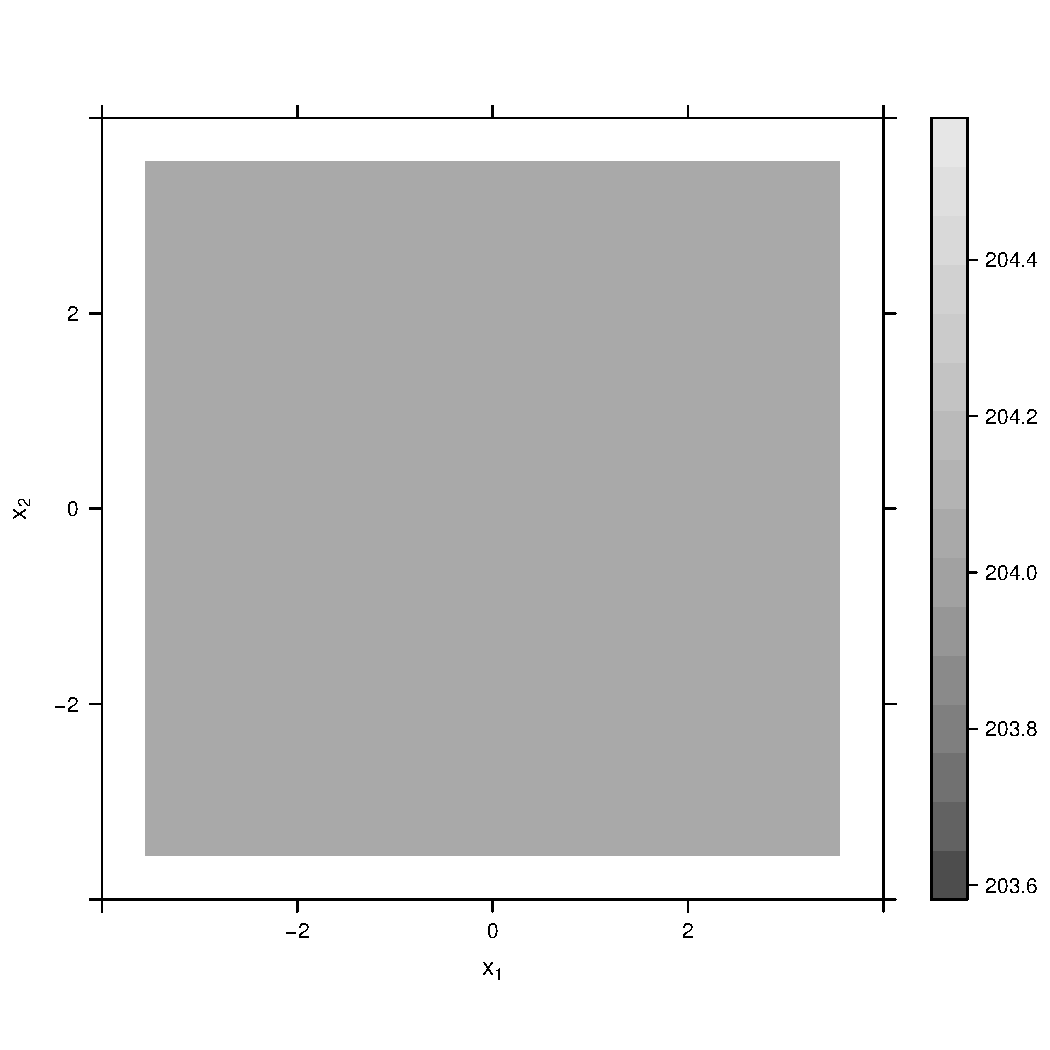
\includegraphics[width=\textwidth]{output/population-heatmap}
    \subcaption{Population distribution}
    \end{subfigure}
    \begin{subfigure}[t]{0.33\textwidth}
    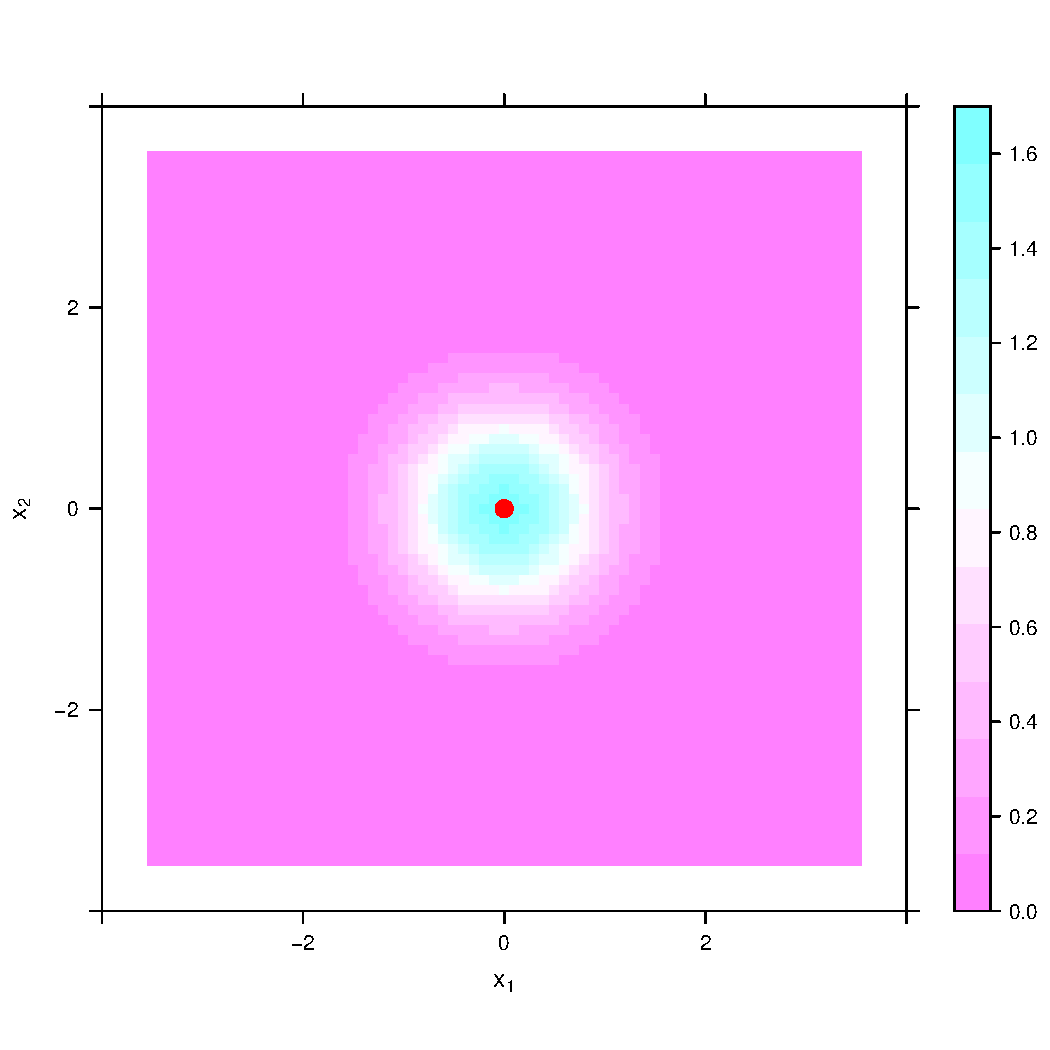
\includegraphics[width=\textwidth]{output/true_intensity_heatmap}
    \subcaption{True risk function}
    \end{subfigure}%
    \begin{subfigure}[t]{0.32\textwidth}
    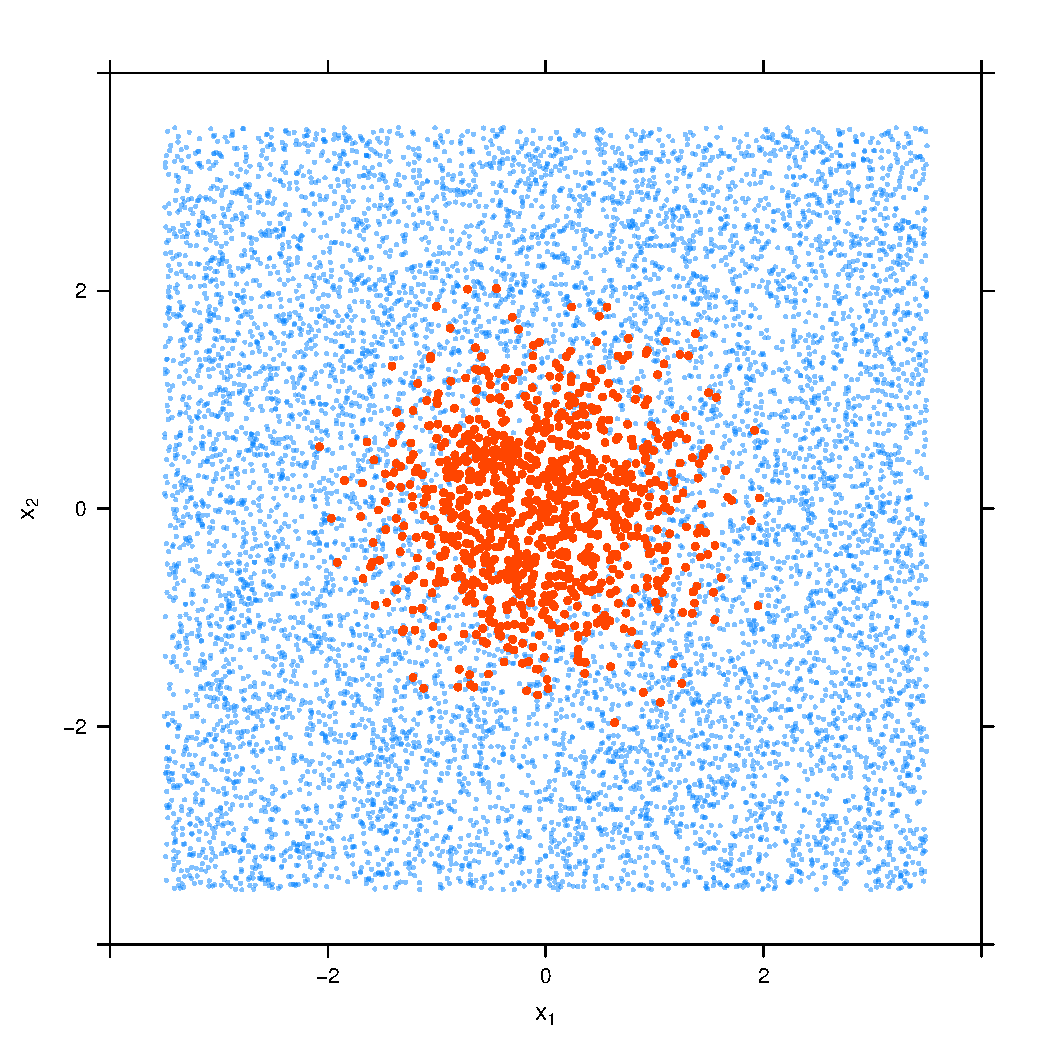
\includegraphics[width=\textwidth]{output/population_and_incidents_scatter}
    \subcaption{Population points (gray) with incidents (black)}
    \end{subfigure}%

    \caption[]{Population distribution (a), true risk function (b), and sample population with incidents (c) for uniform population of 10,000, single-peak risk of decay rate 0.7 and factor 1,000}
    \label{fig:distributions:unif_1000_0.7_1h}    
\end{figure}

%%
%% Section containing single-peak risk with decay rate 1.0 on uniform population
%%
\section{Single-peak risk with decay rate 1.0 on a uniform population}
\label{sec:app:results_unif_1.0_1h}

%%
%% Tables and figures for uniform population of 10,000, single-peak risk of decay rate 1.0, factor 50
%%
\graphicspath{{./results/unif_50_1.0_1h/}}
\makeatletter
\def\input@path{{./results/unif_50_1.0_1h/}}
\makeatother

\begin{table}[H]
        \centering
    \tiny
    \begin{subtable}[t]{0.5\textwidth}
        \centering
        \subcaption{Means} 
        % latex table generated in R 3.4.2 by xtable 1.8-2 package
% Sat Feb 17 16:44:44 2018
\begin{tabular}{lrrr}
  \hline
 & Oracle & Silverman & CV \\ 
  \hline
MISE & 0.000053 & 0.000083 & 0.000080 \\ 
  Relative MISE & 0.002028 & 0.003195 & 0.003047 \\ 
  Normalized MISE & 0.000026 & 0.000042 & 0.000040 \\ 
  MIAE & 0.003914 & 0.004863 & 0.004653 \\ 
  Relative MIAE & 0.024227 & 0.030102 & 0.028802 \\ 
  Max Error & 0.033855 & 0.049415 & 0.045884 \\ 
  Peak bias & -0.016050 & 0.010816 & -0.002953 \\ 
  Relative Peak bias & -0.099339 & 0.066949 & -0.018278 \\ 
  Peak drift & 0.223424 & 0.357624 & 0.284159 \\ 
  Relative Peak drift & 0.031918 & 0.051089 & 0.040594 \\ 
  Centroid bias & -0.017140 & -0.000902 & -0.013918 \\ 
  Relative Centroid bias & -0.106087 & -0.005583 & -0.086149 \\ 
  Centroid drift & 0.149249 & 0.159867 & 0.152694 \\ 
  Relative Centroid drift & 0.021321 & 0.022838 & 0.021813 \\ 
   \hline
\end{tabular}

    \end{subtable}%
    \begin{subtable}[t]{0.5\textwidth}
        \centering
        \subcaption{Standard deviations} 
        % latex table generated in R 3.4.3 by xtable 1.8-2 package
% Sun Apr 15 09:09:45 2018
\begin{tabular}{lrrr}
  \toprule
 & Oracle & Silverman & CV \\ 
  \midrule
MISE & 0.000014 & 0.000014 & 0.000021 \\ 
  Relative MISE & 0.001962 & 0.002039 & 0.003010 \\ 
  Normalized MISE & 0.344229 & 0.357804 & 0.528098 \\ 
  MIAE & 0.000689 & 0.000597 & 0.000961 \\ 
  Relative MIAE & 0.008228 & 0.007121 & 0.011473 \\ 
  Normalized MIAE & 0.000003 & 0.000003 & 0.000005 \\ 
  Supremum error & 0.005321 & 0.006343 & 0.008947 \\ 
  Normalized Sup error & 0.000027 & 0.000032 & 0.000045 \\ 
  Peak bias & 0.008408 & 0.012518 & 0.015040 \\ 
  Relative Peak bias & 0.100360 & 0.149419 & 0.179526 \\ 
  Peak drift & 0.186254 & 0.253752 & 0.225627 \\ 
  Relative Peak drift & 0.026608 & 0.036250 & 0.032232 \\ 
  Centroid bias & 0.008526 & 0.013326 & 0.013412 \\ 
  Relative Centroid bias & 0.101772 & 0.159063 & 0.160095 \\ 
  Centroid drift & 0.142123 & 0.159726 & 0.144847 \\ 
  Relative Centroid drift & 0.020303 & 0.022818 & 0.020692 \\ 
   \bottomrule
\end{tabular}

    \end{subtable}

    \caption[]{Error rates for uniform population of 10,000, single-peak risk of decay rate 1.0 and factor 50}
    \label{tab:mean_error_rates:unif_50_1.0_1h}
\end{table}

\begin{figure}[H]
        \centering
    \begin{subfigure}[t]{0.33\textwidth}
    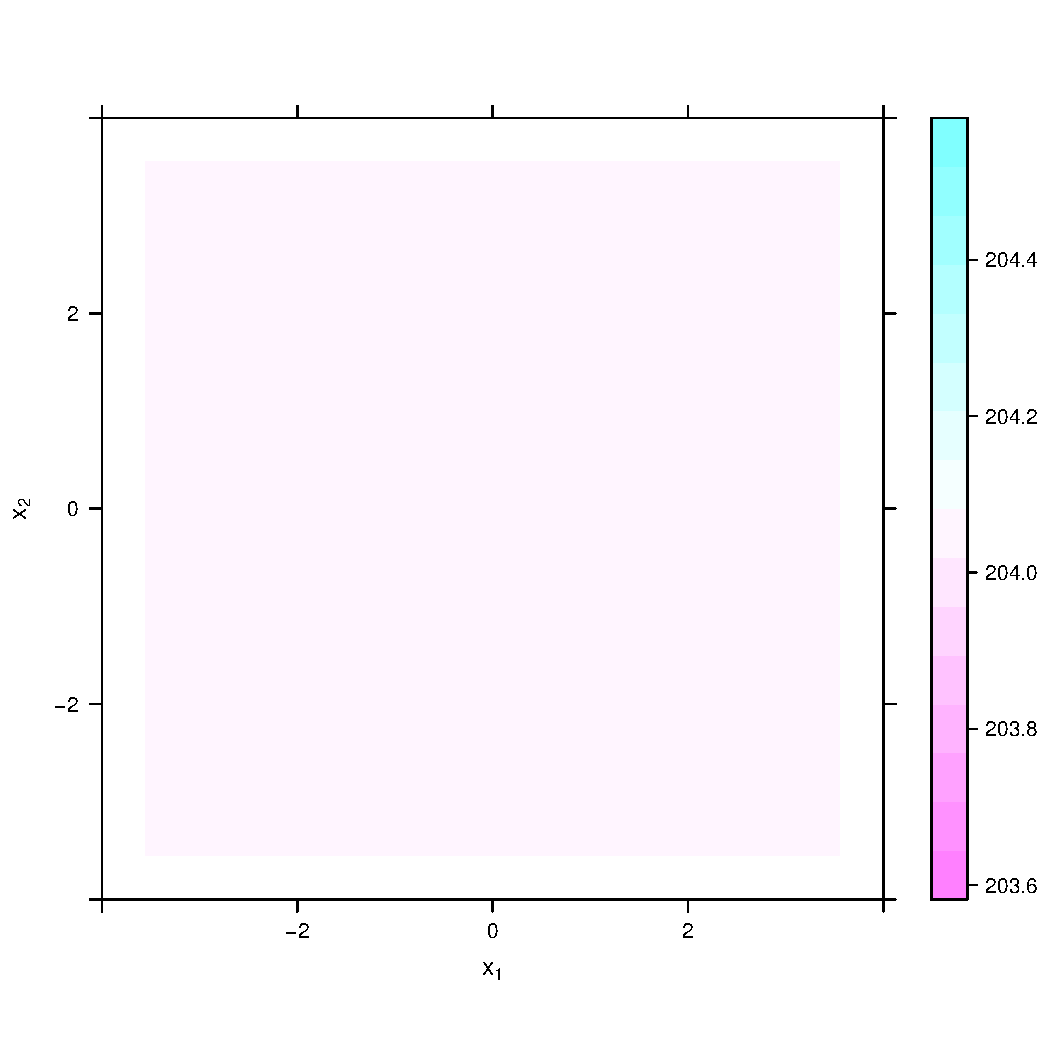
\includegraphics[width=\textwidth]{output/population-heatmap}
    \subcaption{Population distribution}
    \end{subfigure}
    \begin{subfigure}[t]{0.33\textwidth}
    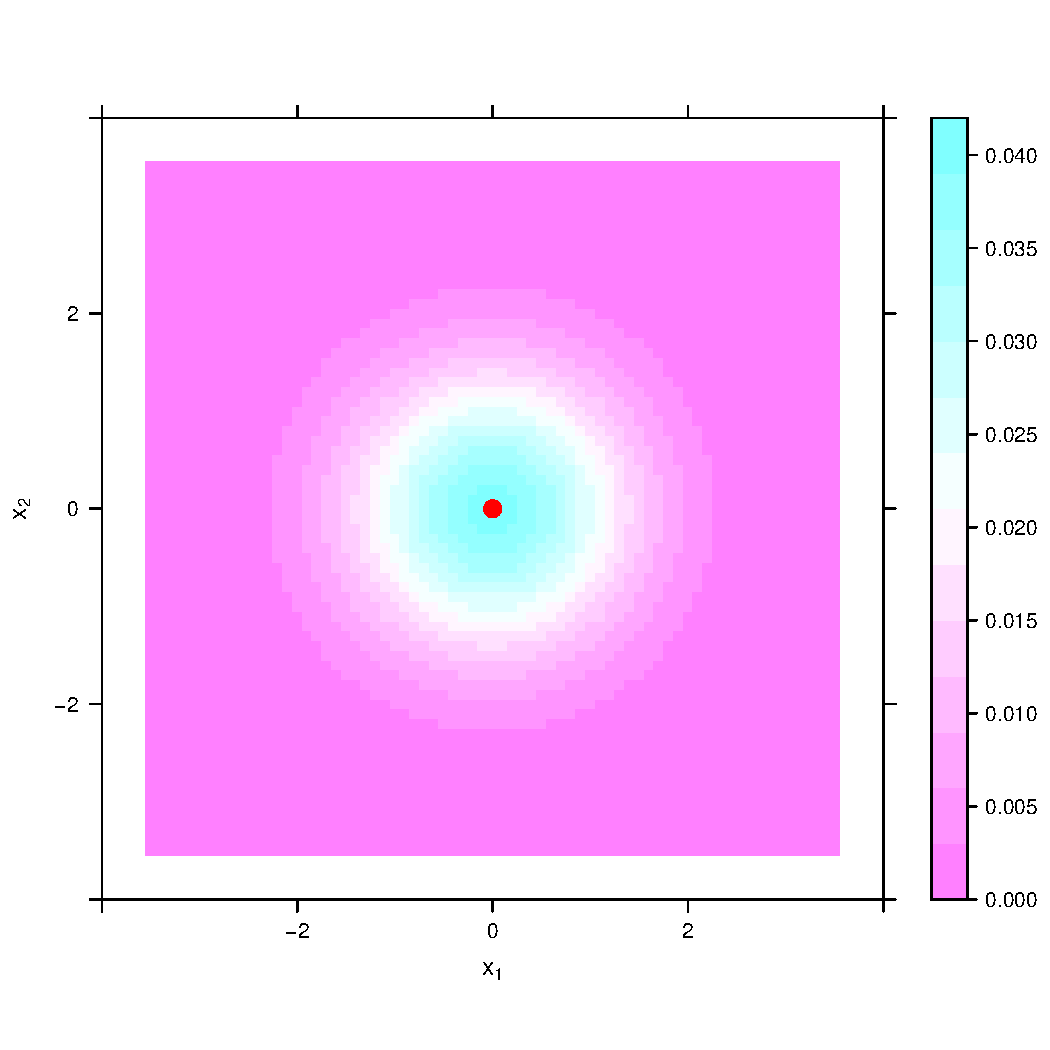
\includegraphics[width=\textwidth]{output/true_intensity_heatmap}
    \subcaption{True risk function}
    \end{subfigure}%
    \begin{subfigure}[t]{0.32\textwidth}
    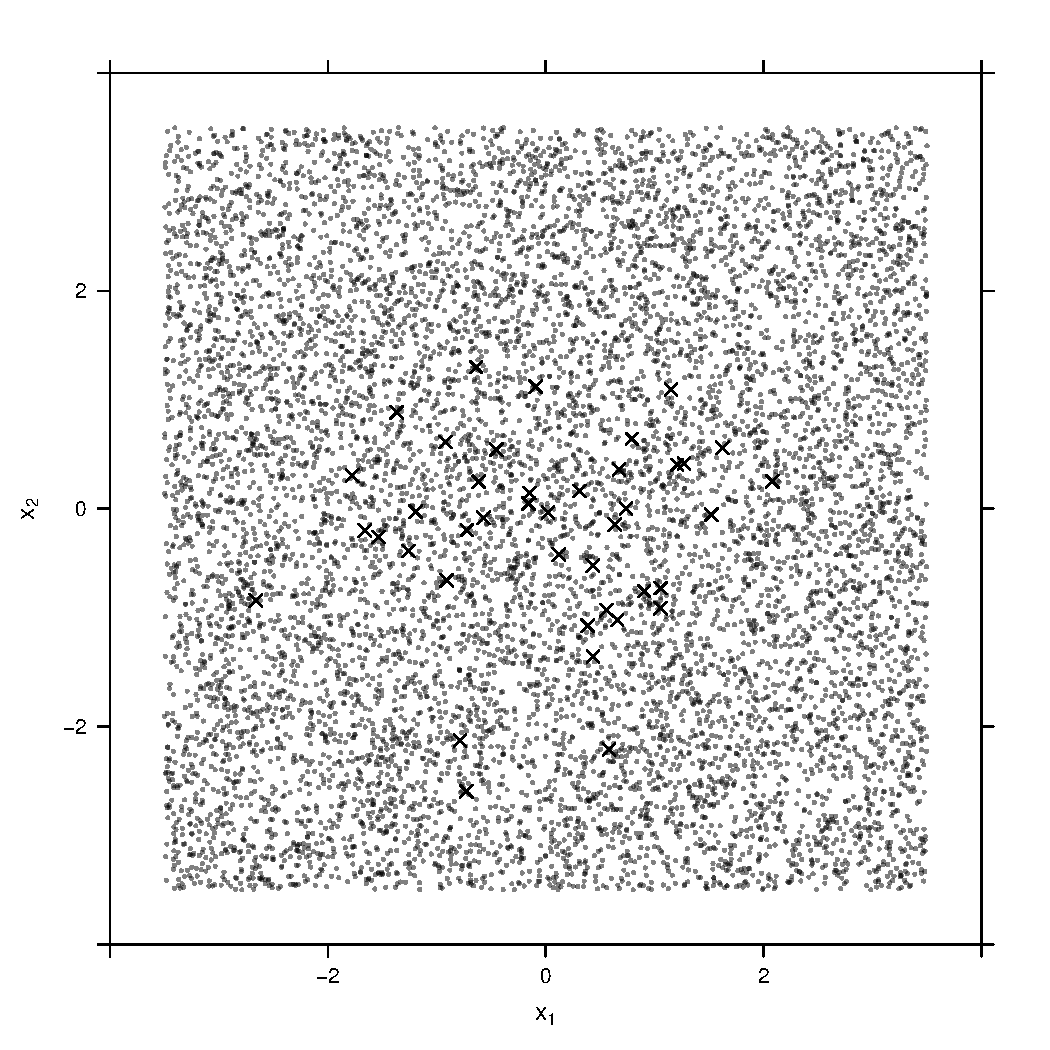
\includegraphics[width=\textwidth]{output/population_and_incidents_scatter}
    \subcaption{Population points (gray) with incidents (black)}
    \end{subfigure}%

    \caption[]{Population distribution (a), true risk function (b), and sample population with incidents (c) for uniform population of 10,000, single-peak risk of decay rate 1.0 and factor 50}
    \label{fig:distributions:unif_50_1.0_1h}    
\end{figure}


%%
%% Tables and figures for uniform population of 10,000, single-peak risk of decay rate 1.0, factor 100
%%
\graphicspath{{./results/unif_100_1.0_1h/}}
\makeatletter
\def\input@path{{./results/unif_100_1.0_1h/}}
\makeatother

\begin{table}[H]
    \centering
    \tiny
    \begin{subtable}[t]{0.5\textwidth}
        \centering
        \subcaption{Means} 
        % latex table generated in R 3.4.2 by xtable 1.8-2 package
% Sat Feb 17 16:44:44 2018
\begin{tabular}{lrrr}
  \hline
 & Oracle & Silverman & CV \\ 
  \hline
MISE & 0.000053 & 0.000083 & 0.000080 \\ 
  Relative MISE & 0.002028 & 0.003195 & 0.003047 \\ 
  Normalized MISE & 0.000026 & 0.000042 & 0.000040 \\ 
  MIAE & 0.003914 & 0.004863 & 0.004653 \\ 
  Relative MIAE & 0.024227 & 0.030102 & 0.028802 \\ 
  Max Error & 0.033855 & 0.049415 & 0.045884 \\ 
  Peak bias & -0.016050 & 0.010816 & -0.002953 \\ 
  Relative Peak bias & -0.099339 & 0.066949 & -0.018278 \\ 
  Peak drift & 0.223424 & 0.357624 & 0.284159 \\ 
  Relative Peak drift & 0.031918 & 0.051089 & 0.040594 \\ 
  Centroid bias & -0.017140 & -0.000902 & -0.013918 \\ 
  Relative Centroid bias & -0.106087 & -0.005583 & -0.086149 \\ 
  Centroid drift & 0.149249 & 0.159867 & 0.152694 \\ 
  Relative Centroid drift & 0.021321 & 0.022838 & 0.021813 \\ 
   \hline
\end{tabular}

    \end{subtable}%
    \begin{subtable}[t]{0.5\textwidth}
        \centering
        \subcaption{Standard deviations} 
        % latex table generated in R 3.4.3 by xtable 1.8-2 package
% Sun Apr 15 09:09:45 2018
\begin{tabular}{lrrr}
  \toprule
 & Oracle & Silverman & CV \\ 
  \midrule
MISE & 0.000014 & 0.000014 & 0.000021 \\ 
  Relative MISE & 0.001962 & 0.002039 & 0.003010 \\ 
  Normalized MISE & 0.344229 & 0.357804 & 0.528098 \\ 
  MIAE & 0.000689 & 0.000597 & 0.000961 \\ 
  Relative MIAE & 0.008228 & 0.007121 & 0.011473 \\ 
  Normalized MIAE & 0.000003 & 0.000003 & 0.000005 \\ 
  Supremum error & 0.005321 & 0.006343 & 0.008947 \\ 
  Normalized Sup error & 0.000027 & 0.000032 & 0.000045 \\ 
  Peak bias & 0.008408 & 0.012518 & 0.015040 \\ 
  Relative Peak bias & 0.100360 & 0.149419 & 0.179526 \\ 
  Peak drift & 0.186254 & 0.253752 & 0.225627 \\ 
  Relative Peak drift & 0.026608 & 0.036250 & 0.032232 \\ 
  Centroid bias & 0.008526 & 0.013326 & 0.013412 \\ 
  Relative Centroid bias & 0.101772 & 0.159063 & 0.160095 \\ 
  Centroid drift & 0.142123 & 0.159726 & 0.144847 \\ 
  Relative Centroid drift & 0.020303 & 0.022818 & 0.020692 \\ 
   \bottomrule
\end{tabular}

    \end{subtable}

\caption[]{Error rates for uniform population of 10,000, single-peak risk of decay rate 1.0 and factor 100}
\label{tab:mean_error_rates:unif_100_1.0_1h}
\end{table}

\begin{figure}[H]
        \centering
    \begin{subfigure}[t]{0.33\textwidth}
    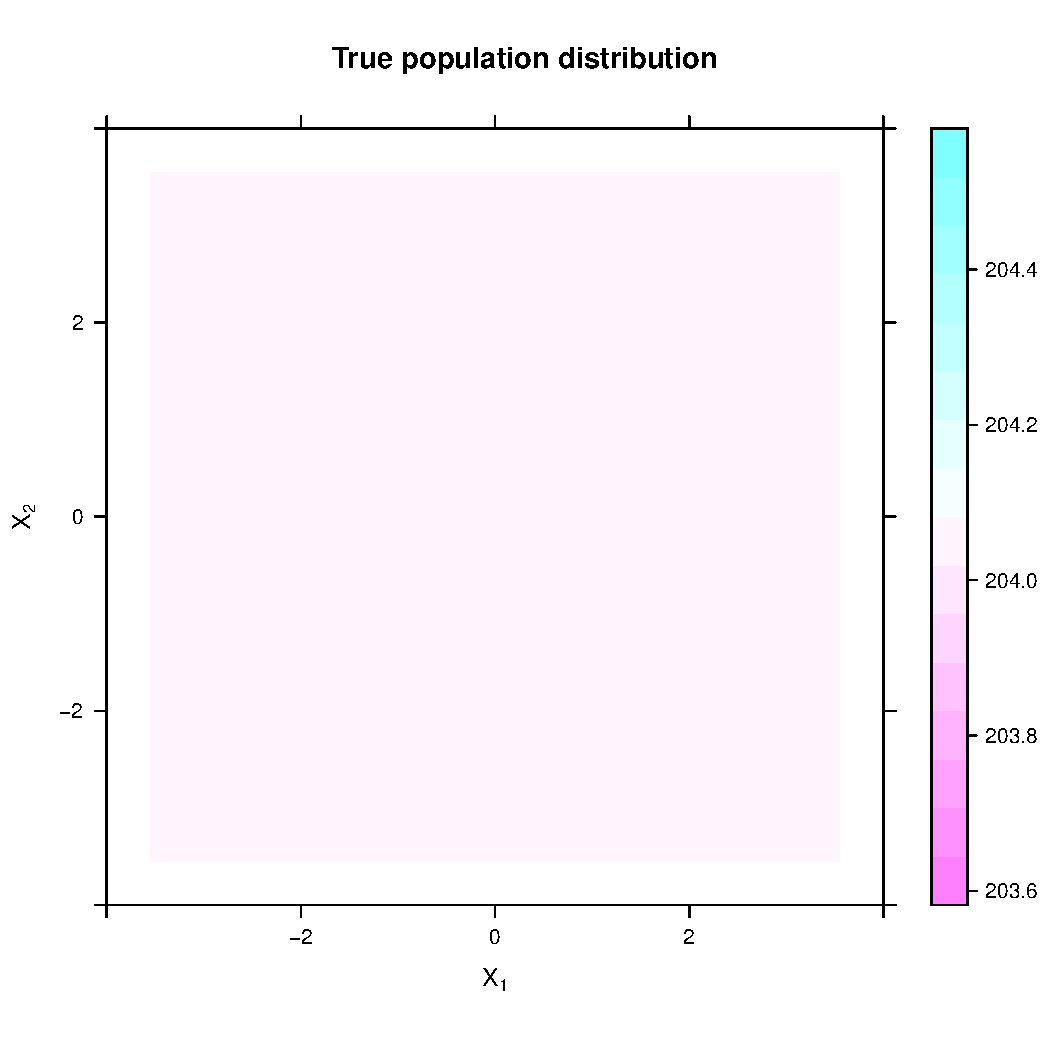
\includegraphics[width=\textwidth]{output/population-heatmap}
    \subcaption{Population distribution}
    \end{subfigure}
    \begin{subfigure}[t]{0.33\textwidth}
    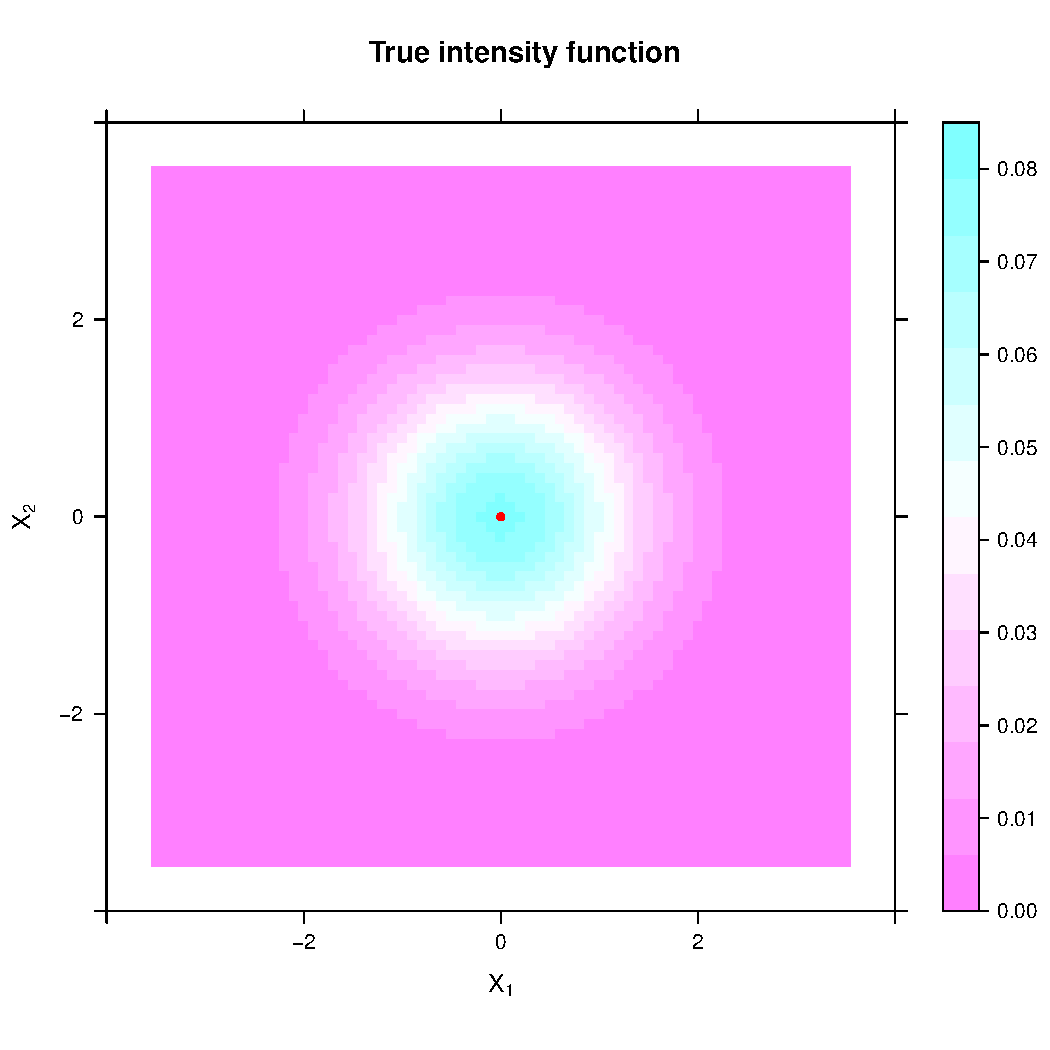
\includegraphics[width=\textwidth]{output/true_intensity_heatmap}
    \subcaption{True risk function}
    \end{subfigure}%
    \begin{subfigure}[t]{0.32\textwidth}
    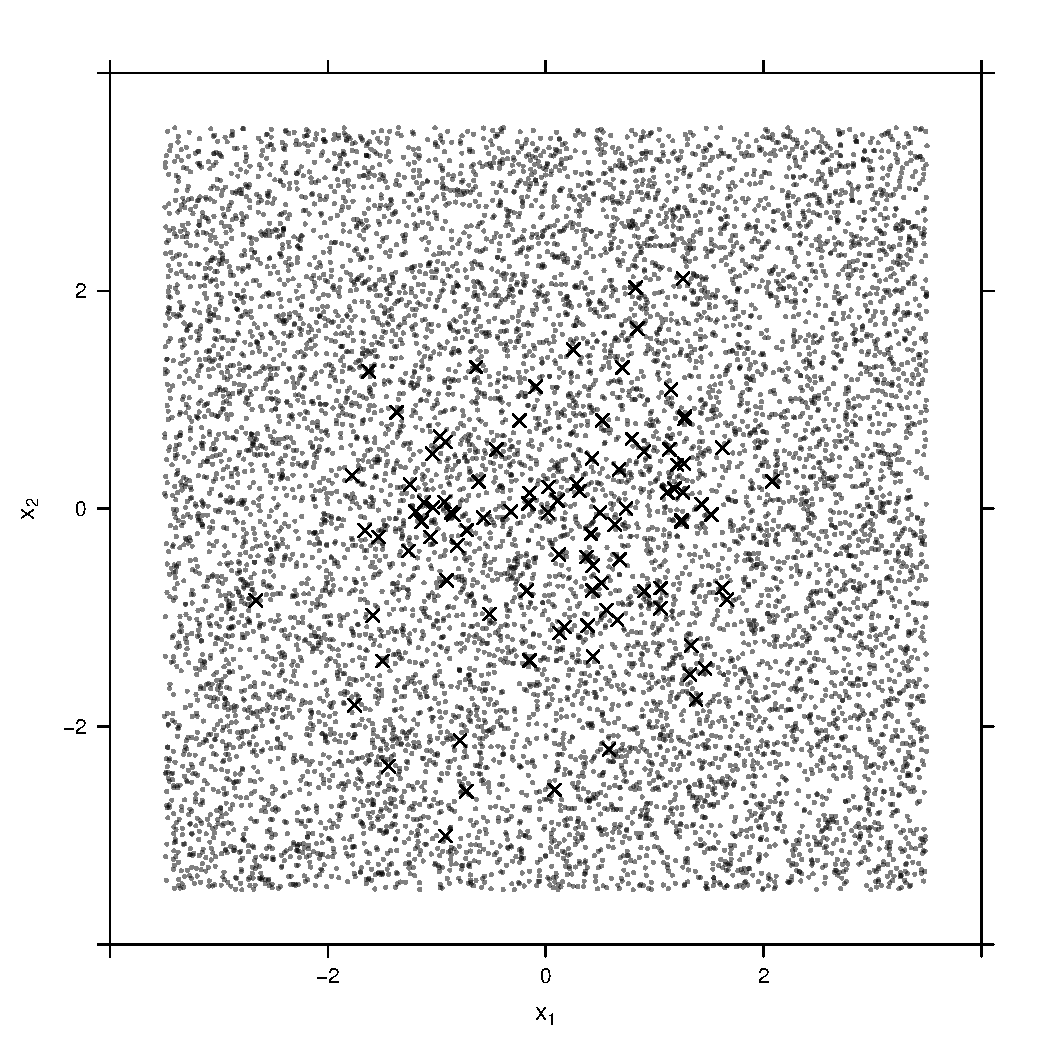
\includegraphics[width=\textwidth]{output/population_and_incidents_scatter}
    \subcaption{Population points (gray) with incidents (black)}
    \end{subfigure}%

    \caption[]{Population distribution (a), true risk function (b), and sample population with incidents (c) for uniform population of 10,000, single-peak risk of decay rate 1.0 and factor 100}
    \label{fig:distributions:unif_100_1.0_1h}    
\end{figure}


%%
%% Tables and figures for uniform population of 10,000, single-peak risk of decay rate 1.0, factor 200
%%
\graphicspath{{./results/unif_200_1.0_1h/}}
\makeatletter
\def\input@path{{./results/unif_200_1.0_1h/}}
\makeatother

\begin{table}[H]
    \centering
    \tiny
    \begin{subtable}[t]{0.5\textwidth}
        \centering
        \subcaption{Means} 
        % latex table generated in R 3.4.2 by xtable 1.8-2 package
% Sat Feb 17 16:44:44 2018
\begin{tabular}{lrrr}
  \hline
 & Oracle & Silverman & CV \\ 
  \hline
MISE & 0.000053 & 0.000083 & 0.000080 \\ 
  Relative MISE & 0.002028 & 0.003195 & 0.003047 \\ 
  Normalized MISE & 0.000026 & 0.000042 & 0.000040 \\ 
  MIAE & 0.003914 & 0.004863 & 0.004653 \\ 
  Relative MIAE & 0.024227 & 0.030102 & 0.028802 \\ 
  Max Error & 0.033855 & 0.049415 & 0.045884 \\ 
  Peak bias & -0.016050 & 0.010816 & -0.002953 \\ 
  Relative Peak bias & -0.099339 & 0.066949 & -0.018278 \\ 
  Peak drift & 0.223424 & 0.357624 & 0.284159 \\ 
  Relative Peak drift & 0.031918 & 0.051089 & 0.040594 \\ 
  Centroid bias & -0.017140 & -0.000902 & -0.013918 \\ 
  Relative Centroid bias & -0.106087 & -0.005583 & -0.086149 \\ 
  Centroid drift & 0.149249 & 0.159867 & 0.152694 \\ 
  Relative Centroid drift & 0.021321 & 0.022838 & 0.021813 \\ 
   \hline
\end{tabular}

    \end{subtable}%
    \begin{subtable}[t]{0.5\textwidth}
        \centering
        \subcaption{Standard deviations} 
        % latex table generated in R 3.4.3 by xtable 1.8-2 package
% Sun Apr 15 09:09:45 2018
\begin{tabular}{lrrr}
  \toprule
 & Oracle & Silverman & CV \\ 
  \midrule
MISE & 0.000014 & 0.000014 & 0.000021 \\ 
  Relative MISE & 0.001962 & 0.002039 & 0.003010 \\ 
  Normalized MISE & 0.344229 & 0.357804 & 0.528098 \\ 
  MIAE & 0.000689 & 0.000597 & 0.000961 \\ 
  Relative MIAE & 0.008228 & 0.007121 & 0.011473 \\ 
  Normalized MIAE & 0.000003 & 0.000003 & 0.000005 \\ 
  Supremum error & 0.005321 & 0.006343 & 0.008947 \\ 
  Normalized Sup error & 0.000027 & 0.000032 & 0.000045 \\ 
  Peak bias & 0.008408 & 0.012518 & 0.015040 \\ 
  Relative Peak bias & 0.100360 & 0.149419 & 0.179526 \\ 
  Peak drift & 0.186254 & 0.253752 & 0.225627 \\ 
  Relative Peak drift & 0.026608 & 0.036250 & 0.032232 \\ 
  Centroid bias & 0.008526 & 0.013326 & 0.013412 \\ 
  Relative Centroid bias & 0.101772 & 0.159063 & 0.160095 \\ 
  Centroid drift & 0.142123 & 0.159726 & 0.144847 \\ 
  Relative Centroid drift & 0.020303 & 0.022818 & 0.020692 \\ 
   \bottomrule
\end{tabular}

    \end{subtable}

\caption[]{Error rates for uniform population of 10,000, single-peak risk of decay rate 1.0 and factor 200}
\label{tab:mean_error_rates:unif_200_1.0_1h}
\end{table}

\begin{figure}[H]
        \centering
    \begin{subfigure}[t]{0.33\textwidth}
    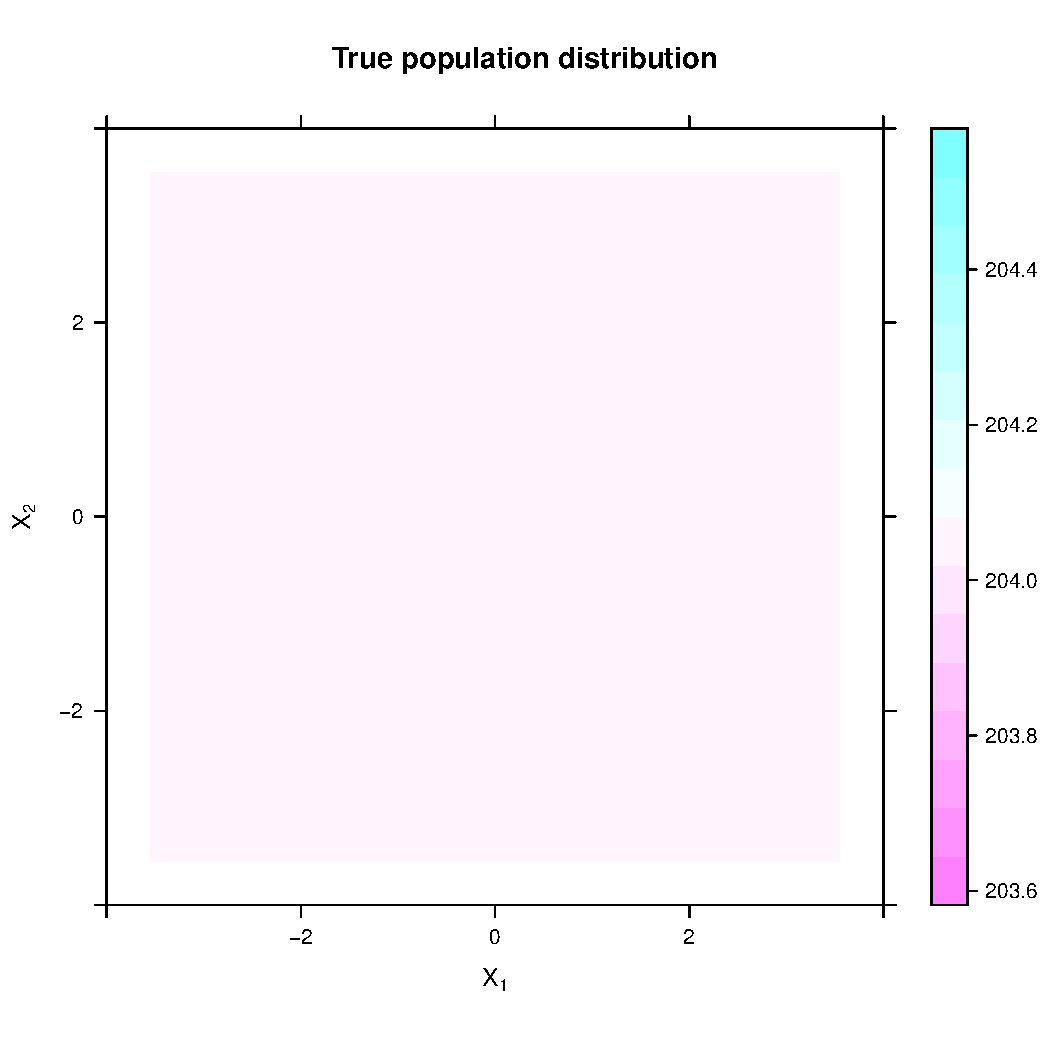
\includegraphics[width=\textwidth]{output/population-heatmap}
    \subcaption{Population distribution}
    \end{subfigure}
    \begin{subfigure}[t]{0.33\textwidth}
    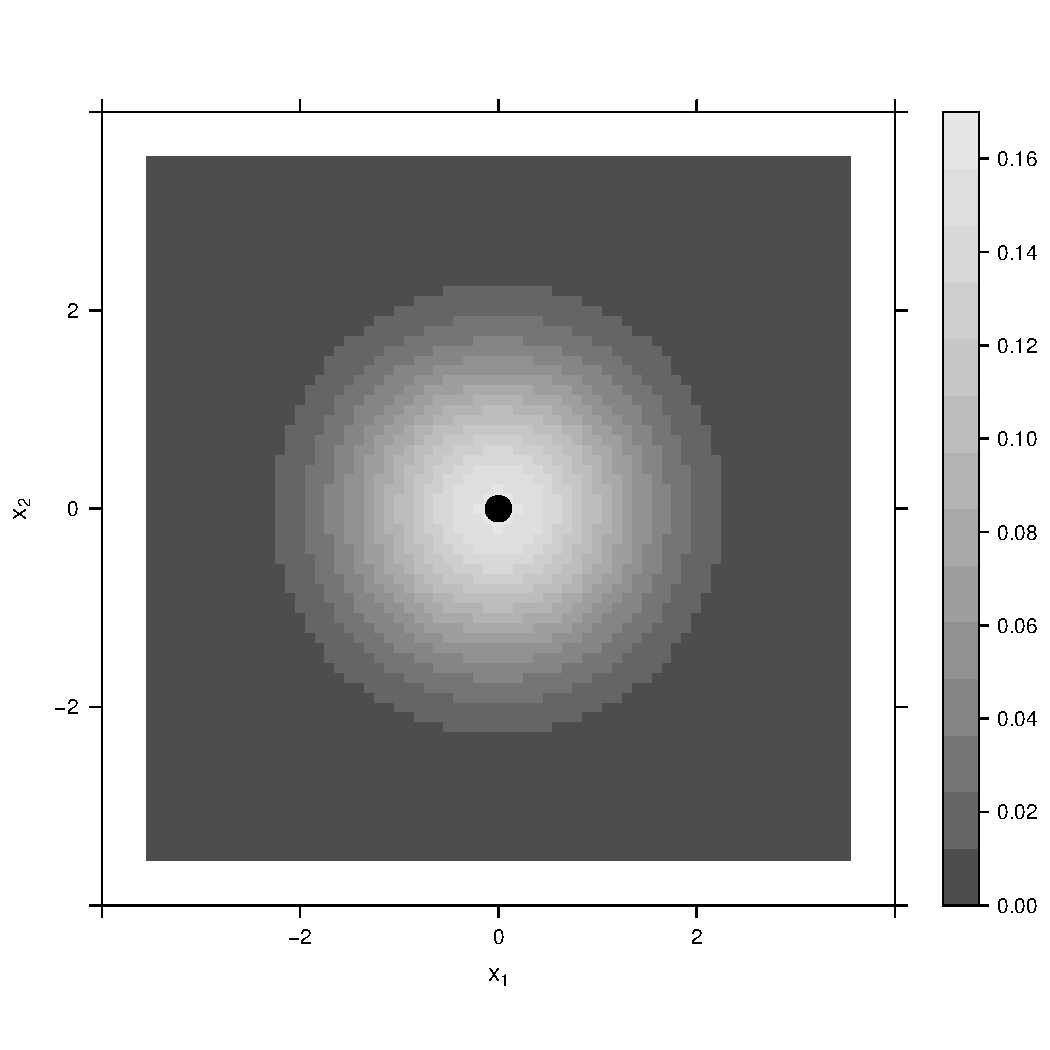
\includegraphics[width=\textwidth]{output/true_intensity_heatmap}
    \subcaption{True risk function}
    \end{subfigure}%
    \begin{subfigure}[t]{0.32\textwidth}
    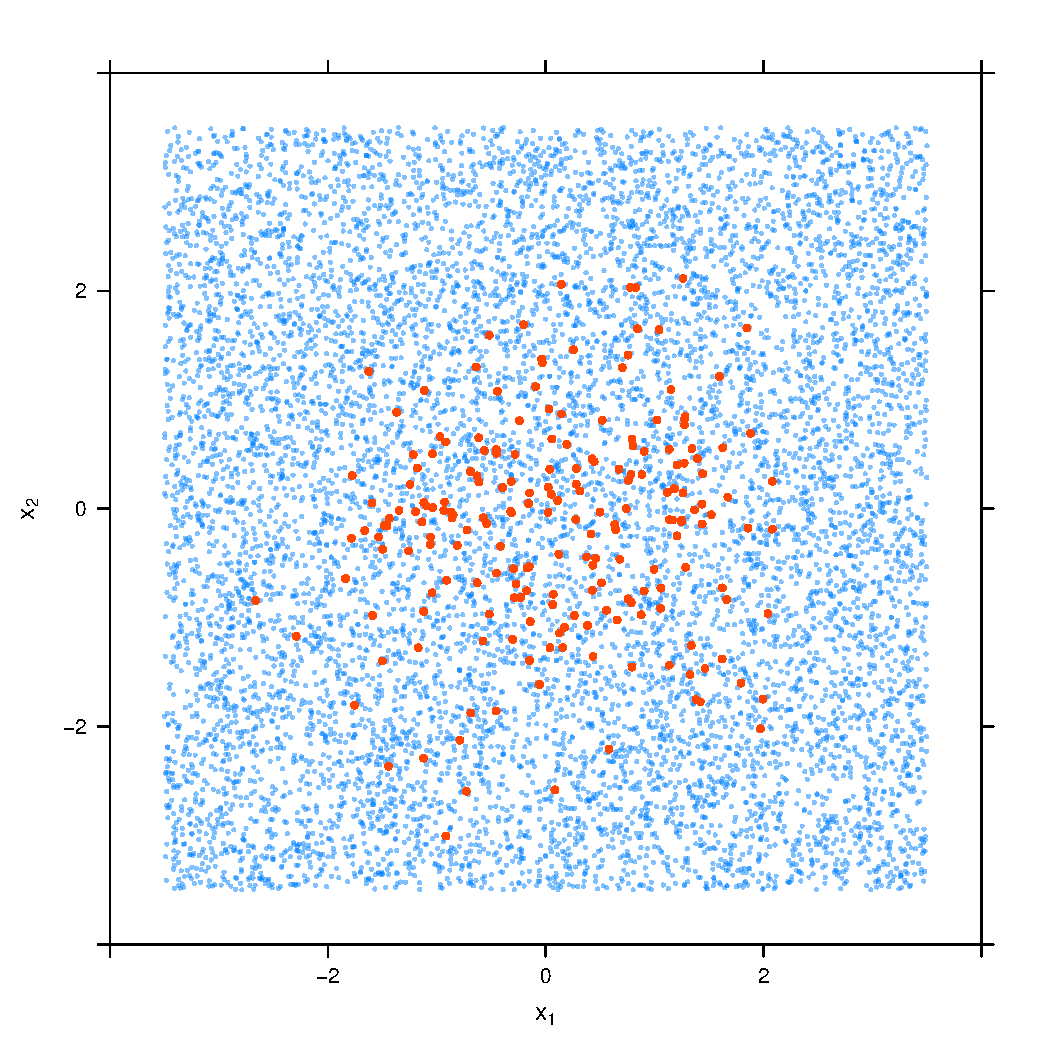
\includegraphics[width=\textwidth]{output/population_and_incidents_scatter}
    \subcaption{Population points (gray) with incidents (black)}
    \end{subfigure}%

    \caption[]{Population distribution (a), true risk function (b), and sample population with incidents (c) for uniform population of 10,000, single-peak risk of decay rate 1.0 and factor 200}
    \label{fig:distributions:unif_200_1.0_1h}    
\end{figure}


%%
%% Tables and figures for uniform population of 10,000, single-peak risk of decay rate 1.0, factor 500
%%
\graphicspath{{./results/unif_500_1.0_1h/}}
\makeatletter
\def\input@path{{./results/unif_500_1.0_1h/}}
\makeatother

\begin{table}[H]
    \centering
    \tiny
    \begin{subtable}[t]{0.5\textwidth}
        \centering
        \subcaption{Means} 
        % latex table generated in R 3.4.2 by xtable 1.8-2 package
% Sat Feb 17 16:44:44 2018
\begin{tabular}{lrrr}
  \hline
 & Oracle & Silverman & CV \\ 
  \hline
MISE & 0.000053 & 0.000083 & 0.000080 \\ 
  Relative MISE & 0.002028 & 0.003195 & 0.003047 \\ 
  Normalized MISE & 0.000026 & 0.000042 & 0.000040 \\ 
  MIAE & 0.003914 & 0.004863 & 0.004653 \\ 
  Relative MIAE & 0.024227 & 0.030102 & 0.028802 \\ 
  Max Error & 0.033855 & 0.049415 & 0.045884 \\ 
  Peak bias & -0.016050 & 0.010816 & -0.002953 \\ 
  Relative Peak bias & -0.099339 & 0.066949 & -0.018278 \\ 
  Peak drift & 0.223424 & 0.357624 & 0.284159 \\ 
  Relative Peak drift & 0.031918 & 0.051089 & 0.040594 \\ 
  Centroid bias & -0.017140 & -0.000902 & -0.013918 \\ 
  Relative Centroid bias & -0.106087 & -0.005583 & -0.086149 \\ 
  Centroid drift & 0.149249 & 0.159867 & 0.152694 \\ 
  Relative Centroid drift & 0.021321 & 0.022838 & 0.021813 \\ 
   \hline
\end{tabular}

    \end{subtable}%
    \begin{subtable}[t]{0.5\textwidth}
        \centering
        \subcaption{Standard deviations} 
        % latex table generated in R 3.4.3 by xtable 1.8-2 package
% Sun Apr 15 09:09:45 2018
\begin{tabular}{lrrr}
  \toprule
 & Oracle & Silverman & CV \\ 
  \midrule
MISE & 0.000014 & 0.000014 & 0.000021 \\ 
  Relative MISE & 0.001962 & 0.002039 & 0.003010 \\ 
  Normalized MISE & 0.344229 & 0.357804 & 0.528098 \\ 
  MIAE & 0.000689 & 0.000597 & 0.000961 \\ 
  Relative MIAE & 0.008228 & 0.007121 & 0.011473 \\ 
  Normalized MIAE & 0.000003 & 0.000003 & 0.000005 \\ 
  Supremum error & 0.005321 & 0.006343 & 0.008947 \\ 
  Normalized Sup error & 0.000027 & 0.000032 & 0.000045 \\ 
  Peak bias & 0.008408 & 0.012518 & 0.015040 \\ 
  Relative Peak bias & 0.100360 & 0.149419 & 0.179526 \\ 
  Peak drift & 0.186254 & 0.253752 & 0.225627 \\ 
  Relative Peak drift & 0.026608 & 0.036250 & 0.032232 \\ 
  Centroid bias & 0.008526 & 0.013326 & 0.013412 \\ 
  Relative Centroid bias & 0.101772 & 0.159063 & 0.160095 \\ 
  Centroid drift & 0.142123 & 0.159726 & 0.144847 \\ 
  Relative Centroid drift & 0.020303 & 0.022818 & 0.020692 \\ 
   \bottomrule
\end{tabular}

    \end{subtable}

\caption[]{Error rates for uniform population of 10,000, single-peak risk of decay rate 1.0 and factor 500}
\label{tab:mean_error_rates:unif_500_1.0_1h}
\end{table}

\begin{figure}[H]
        \centering
    \begin{subfigure}[t]{0.33\textwidth}
    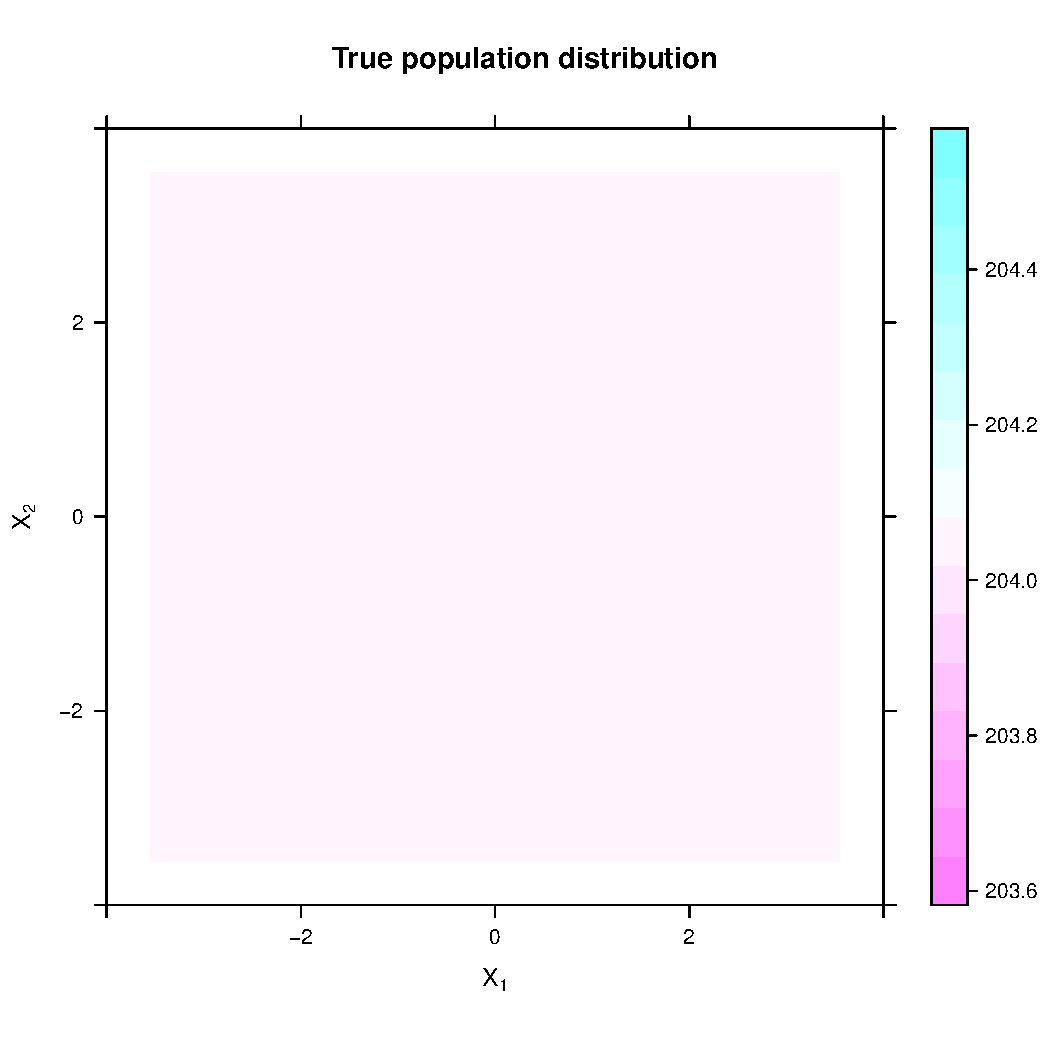
\includegraphics[width=\textwidth]{output/population-heatmap}
    \subcaption{Population distribution}
    \end{subfigure}
    \begin{subfigure}[t]{0.33\textwidth}
    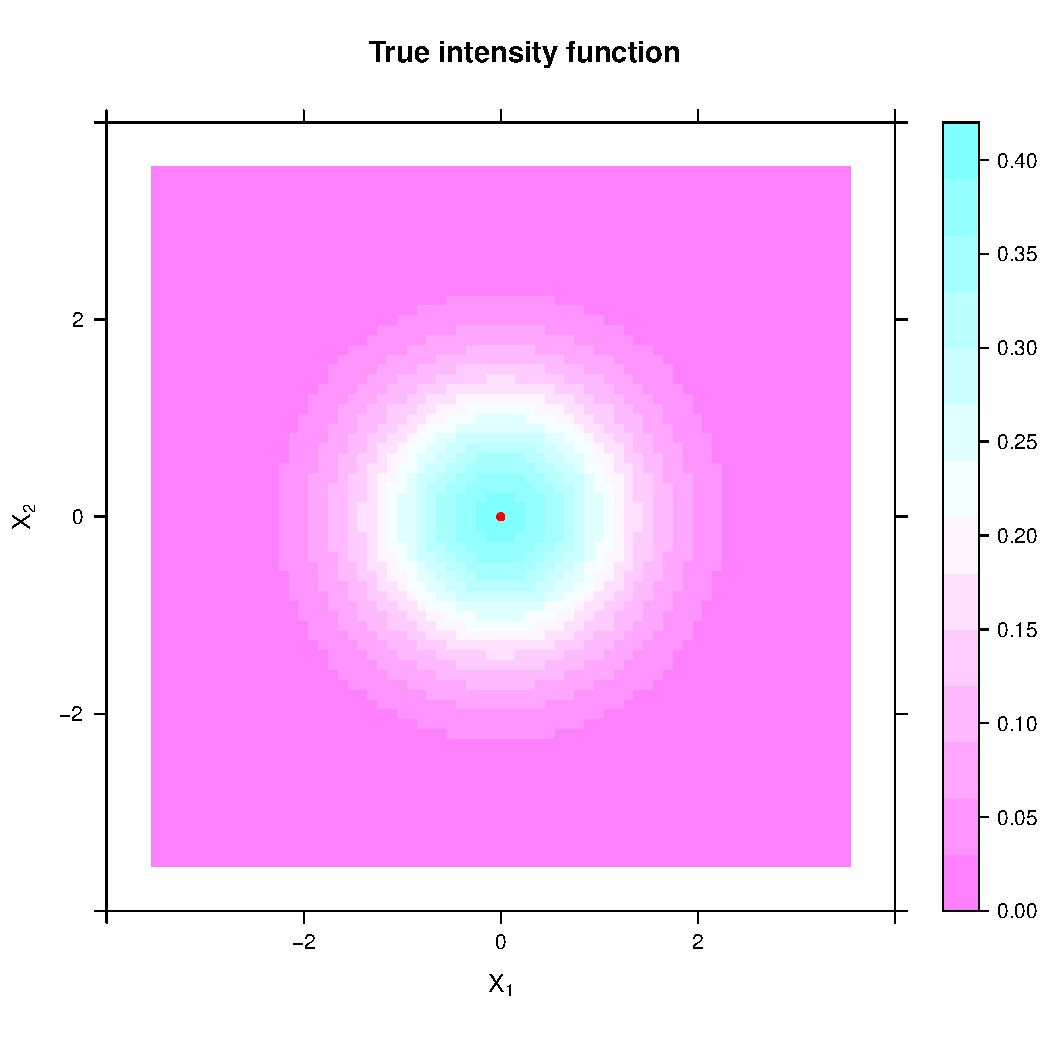
\includegraphics[width=\textwidth]{output/true_intensity_heatmap}
    \subcaption{True risk function}
    \end{subfigure}%
    \begin{subfigure}[t]{0.32\textwidth}
    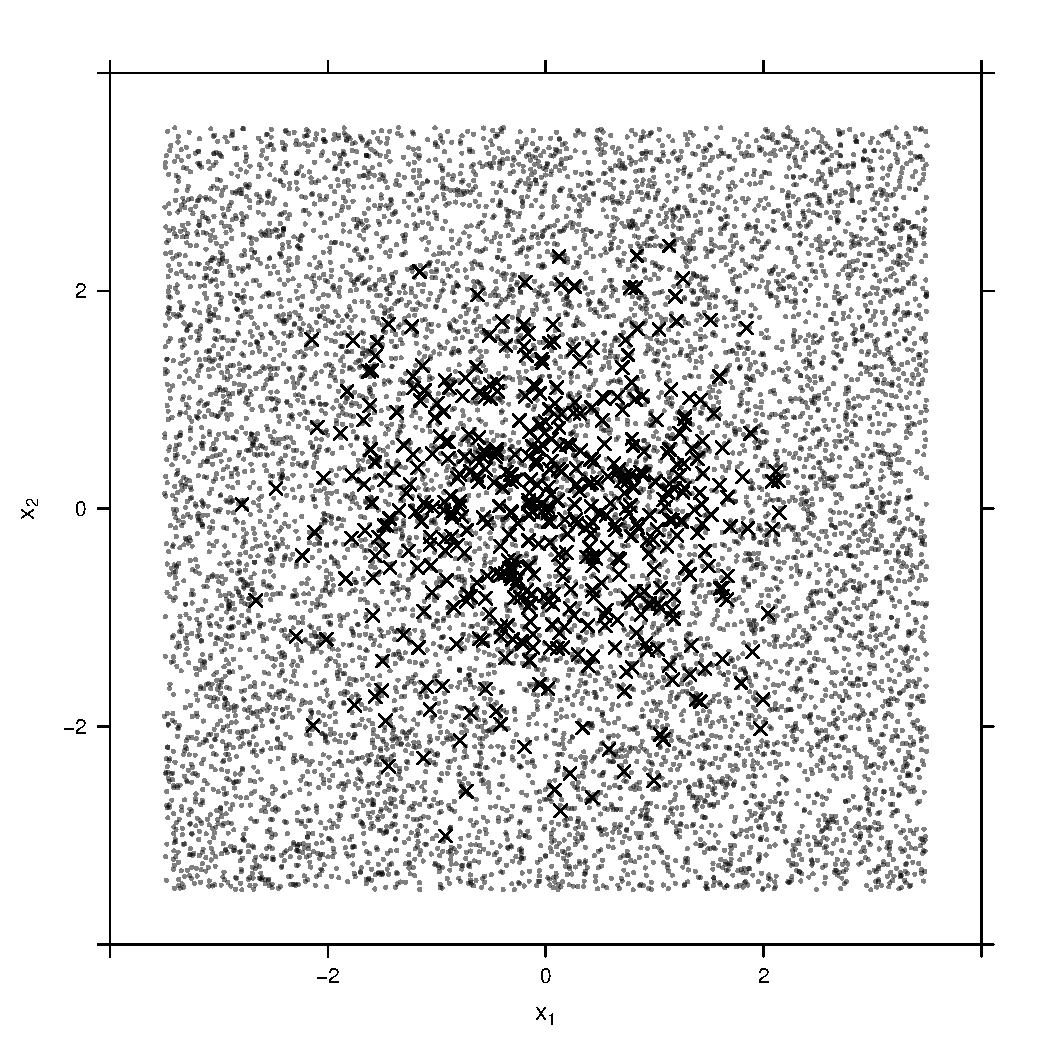
\includegraphics[width=\textwidth]{output/population_and_incidents_scatter}
    \subcaption{Population points (gray) with incidents (black)}
    \end{subfigure}%

    \caption[]{Population distribution (a), true risk function (b), and sample population with incidents (c) for uniform population of 10,000, single-peak risk of decay rate 1.0 and factor 500}
    \label{fig:distributions:unif_500_1.0_1h}    
\end{figure}


%%
%% Tables and figures for uniform population of 10,000, single-peak risk of decay rate 1.0, factor 1,000
%%
\graphicspath{{./results/unif_1000_1.0_1h/}}
\makeatletter
\def\input@path{{./results/unif_1000_1.0_1h/}}
\makeatother

\begin{table}[H]
    \centering
    \tiny
    \begin{subtable}[t]{0.5\textwidth}
        \centering
        \subcaption{Means} 
        % latex table generated in R 3.4.2 by xtable 1.8-2 package
% Sat Feb 17 16:44:44 2018
\begin{tabular}{lrrr}
  \hline
 & Oracle & Silverman & CV \\ 
  \hline
MISE & 0.000053 & 0.000083 & 0.000080 \\ 
  Relative MISE & 0.002028 & 0.003195 & 0.003047 \\ 
  Normalized MISE & 0.000026 & 0.000042 & 0.000040 \\ 
  MIAE & 0.003914 & 0.004863 & 0.004653 \\ 
  Relative MIAE & 0.024227 & 0.030102 & 0.028802 \\ 
  Max Error & 0.033855 & 0.049415 & 0.045884 \\ 
  Peak bias & -0.016050 & 0.010816 & -0.002953 \\ 
  Relative Peak bias & -0.099339 & 0.066949 & -0.018278 \\ 
  Peak drift & 0.223424 & 0.357624 & 0.284159 \\ 
  Relative Peak drift & 0.031918 & 0.051089 & 0.040594 \\ 
  Centroid bias & -0.017140 & -0.000902 & -0.013918 \\ 
  Relative Centroid bias & -0.106087 & -0.005583 & -0.086149 \\ 
  Centroid drift & 0.149249 & 0.159867 & 0.152694 \\ 
  Relative Centroid drift & 0.021321 & 0.022838 & 0.021813 \\ 
   \hline
\end{tabular}

    \end{subtable}%
    \begin{subtable}[t]{0.5\textwidth}
        \centering
        \subcaption{Standard deviations} 
        % latex table generated in R 3.4.3 by xtable 1.8-2 package
% Sun Apr 15 09:09:45 2018
\begin{tabular}{lrrr}
  \toprule
 & Oracle & Silverman & CV \\ 
  \midrule
MISE & 0.000014 & 0.000014 & 0.000021 \\ 
  Relative MISE & 0.001962 & 0.002039 & 0.003010 \\ 
  Normalized MISE & 0.344229 & 0.357804 & 0.528098 \\ 
  MIAE & 0.000689 & 0.000597 & 0.000961 \\ 
  Relative MIAE & 0.008228 & 0.007121 & 0.011473 \\ 
  Normalized MIAE & 0.000003 & 0.000003 & 0.000005 \\ 
  Supremum error & 0.005321 & 0.006343 & 0.008947 \\ 
  Normalized Sup error & 0.000027 & 0.000032 & 0.000045 \\ 
  Peak bias & 0.008408 & 0.012518 & 0.015040 \\ 
  Relative Peak bias & 0.100360 & 0.149419 & 0.179526 \\ 
  Peak drift & 0.186254 & 0.253752 & 0.225627 \\ 
  Relative Peak drift & 0.026608 & 0.036250 & 0.032232 \\ 
  Centroid bias & 0.008526 & 0.013326 & 0.013412 \\ 
  Relative Centroid bias & 0.101772 & 0.159063 & 0.160095 \\ 
  Centroid drift & 0.142123 & 0.159726 & 0.144847 \\ 
  Relative Centroid drift & 0.020303 & 0.022818 & 0.020692 \\ 
   \bottomrule
\end{tabular}

    \end{subtable}

\caption[]{Error rates for uniform population of 10,000, single-peak risk of decay rate 1.0 and factor 1,000}
\label{tab:mean_error_rates:unif_1000_1.0_1h}
\end{table}

\begin{figure}[H]
        \centering
    \begin{subfigure}[t]{0.33\textwidth}
    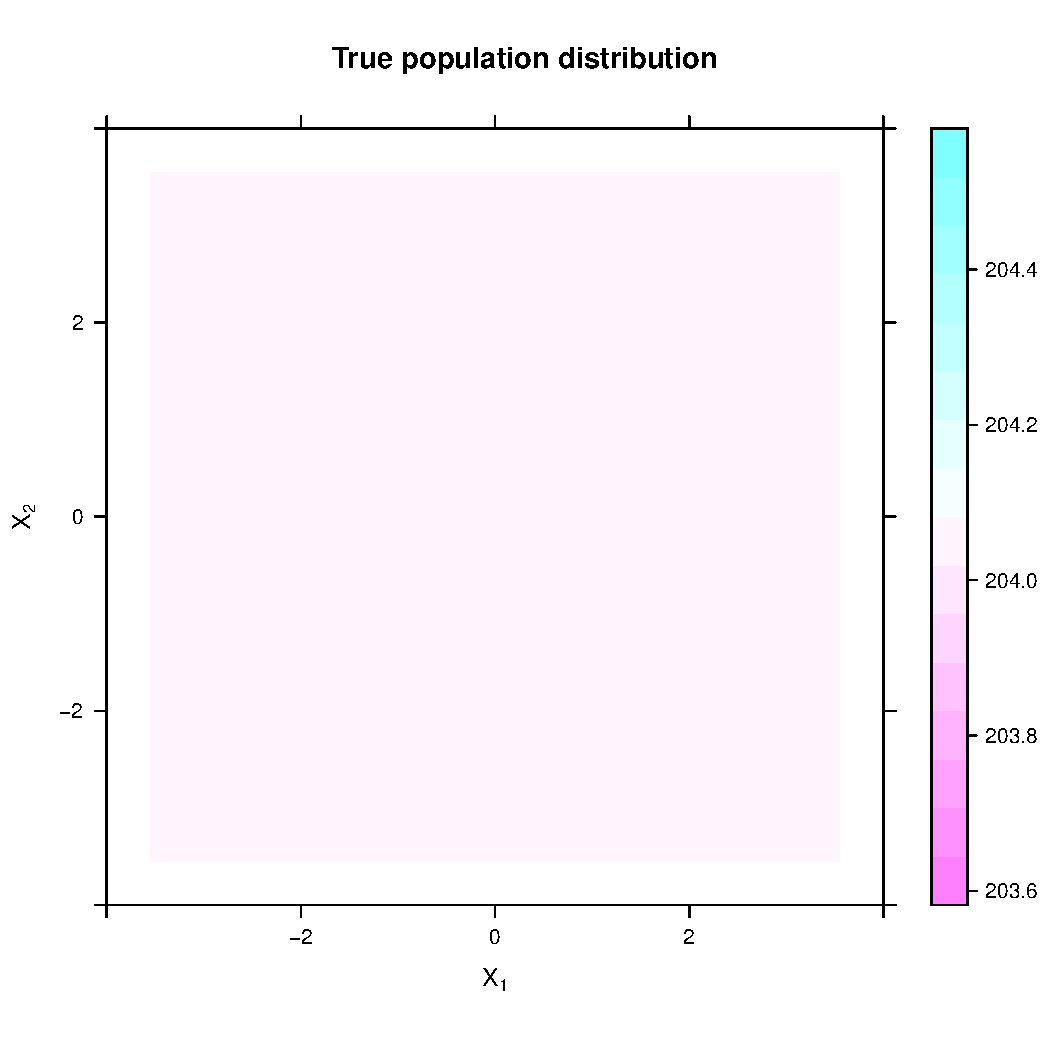
\includegraphics[width=\textwidth]{output/population-heatmap}
    \subcaption{Population distribution}
    \end{subfigure}
    \begin{subfigure}[t]{0.33\textwidth}
    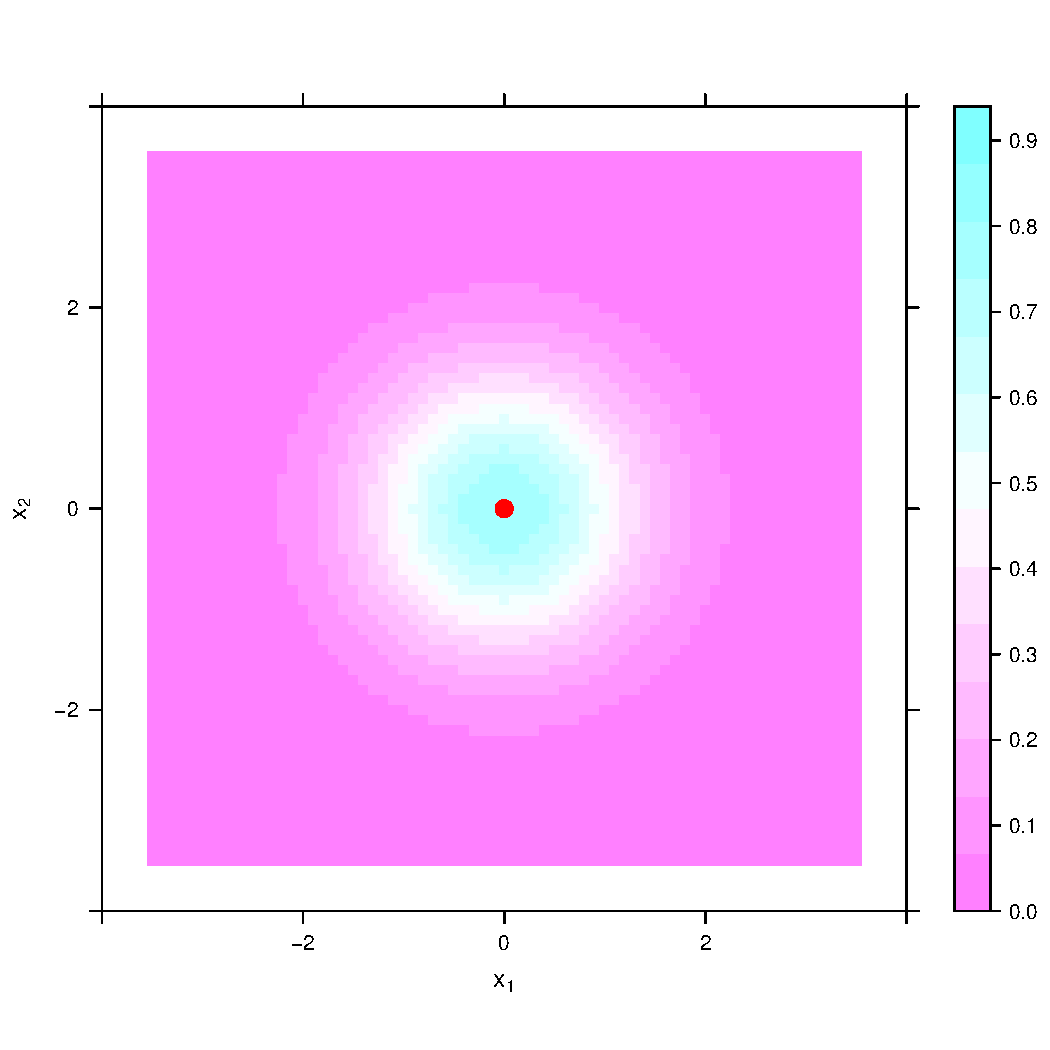
\includegraphics[width=\textwidth]{output/true_intensity_heatmap}
    \subcaption{True risk function}
    \end{subfigure}%
    \begin{subfigure}[t]{0.32\textwidth}
    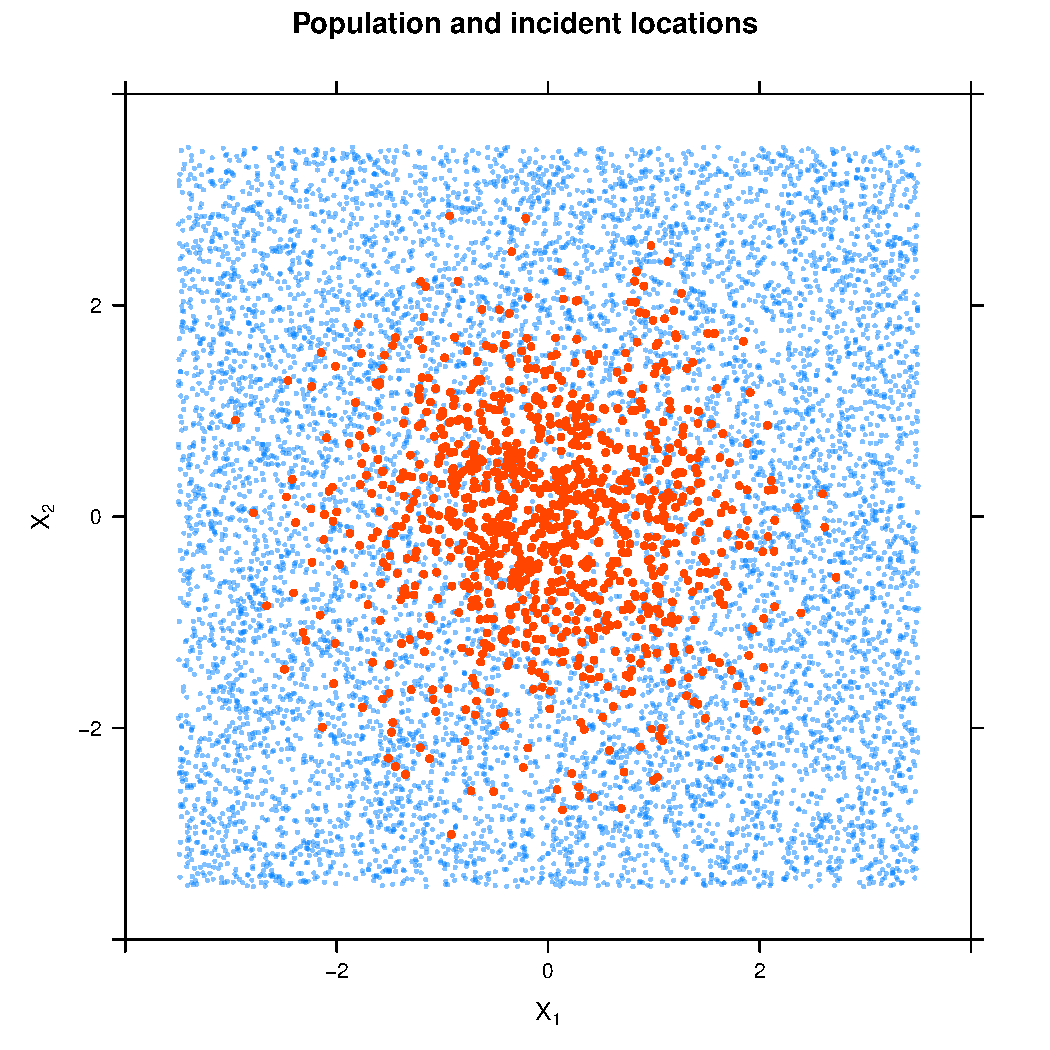
\includegraphics[width=\textwidth]{output/population_and_incidents_scatter}
    \subcaption{Population points (gray) with incidents (black)}
    \end{subfigure}%

    \caption[]{Population distribution (a), true risk function (b), and sample population with incidents (c) for uniform population of 10,000, single-peak risk of decay rate 1.0 and factor 1,000}
    \label{fig:distributions:unif_1000_1.0_1h}    
\end{figure}

 
%%
%% Section containing single-peak risk with decay rate 1.4 on uniform population
%%
\section{Single-peak risk with decay rate 1.4 on a uniform population}
\label{sec:app:results_unif_1.4_1h}

%%
%% Tables and figures for uniform population of 10,000, single-peak risk of decay rate 1.4, factor 50
%%
\graphicspath{{./results/unif_50_1.4_1h/}}
\makeatletter
\def\input@path{{./results/unif_50_1.4_1h/}}
\makeatother

\begin{table}[H]
        \centering
    \tiny
    \begin{subtable}[t]{0.5\textwidth}
        \centering
        \subcaption{Means} 
        % latex table generated in R 3.4.2 by xtable 1.8-2 package
% Sat Feb 17 16:44:44 2018
\begin{tabular}{lrrr}
  \hline
 & Oracle & Silverman & CV \\ 
  \hline
MISE & 0.000053 & 0.000083 & 0.000080 \\ 
  Relative MISE & 0.002028 & 0.003195 & 0.003047 \\ 
  Normalized MISE & 0.000026 & 0.000042 & 0.000040 \\ 
  MIAE & 0.003914 & 0.004863 & 0.004653 \\ 
  Relative MIAE & 0.024227 & 0.030102 & 0.028802 \\ 
  Max Error & 0.033855 & 0.049415 & 0.045884 \\ 
  Peak bias & -0.016050 & 0.010816 & -0.002953 \\ 
  Relative Peak bias & -0.099339 & 0.066949 & -0.018278 \\ 
  Peak drift & 0.223424 & 0.357624 & 0.284159 \\ 
  Relative Peak drift & 0.031918 & 0.051089 & 0.040594 \\ 
  Centroid bias & -0.017140 & -0.000902 & -0.013918 \\ 
  Relative Centroid bias & -0.106087 & -0.005583 & -0.086149 \\ 
  Centroid drift & 0.149249 & 0.159867 & 0.152694 \\ 
  Relative Centroid drift & 0.021321 & 0.022838 & 0.021813 \\ 
   \hline
\end{tabular}

    \end{subtable}%
    \begin{subtable}[t]{0.5\textwidth}
        \centering
        \subcaption{Standard deviations} 
        % latex table generated in R 3.4.3 by xtable 1.8-2 package
% Sun Apr 15 09:09:45 2018
\begin{tabular}{lrrr}
  \toprule
 & Oracle & Silverman & CV \\ 
  \midrule
MISE & 0.000014 & 0.000014 & 0.000021 \\ 
  Relative MISE & 0.001962 & 0.002039 & 0.003010 \\ 
  Normalized MISE & 0.344229 & 0.357804 & 0.528098 \\ 
  MIAE & 0.000689 & 0.000597 & 0.000961 \\ 
  Relative MIAE & 0.008228 & 0.007121 & 0.011473 \\ 
  Normalized MIAE & 0.000003 & 0.000003 & 0.000005 \\ 
  Supremum error & 0.005321 & 0.006343 & 0.008947 \\ 
  Normalized Sup error & 0.000027 & 0.000032 & 0.000045 \\ 
  Peak bias & 0.008408 & 0.012518 & 0.015040 \\ 
  Relative Peak bias & 0.100360 & 0.149419 & 0.179526 \\ 
  Peak drift & 0.186254 & 0.253752 & 0.225627 \\ 
  Relative Peak drift & 0.026608 & 0.036250 & 0.032232 \\ 
  Centroid bias & 0.008526 & 0.013326 & 0.013412 \\ 
  Relative Centroid bias & 0.101772 & 0.159063 & 0.160095 \\ 
  Centroid drift & 0.142123 & 0.159726 & 0.144847 \\ 
  Relative Centroid drift & 0.020303 & 0.022818 & 0.020692 \\ 
   \bottomrule
\end{tabular}

    \end{subtable}

    \caption[]{Error rates for uniform population of 10,000, single-peak risk of decay rate 1.4 and factor 50}
    \label{tab:mean_error_rates:unif_50_1.4_1h}
\end{table}

\begin{figure}[H]
        \centering
    \begin{subfigure}[t]{0.33\textwidth}
    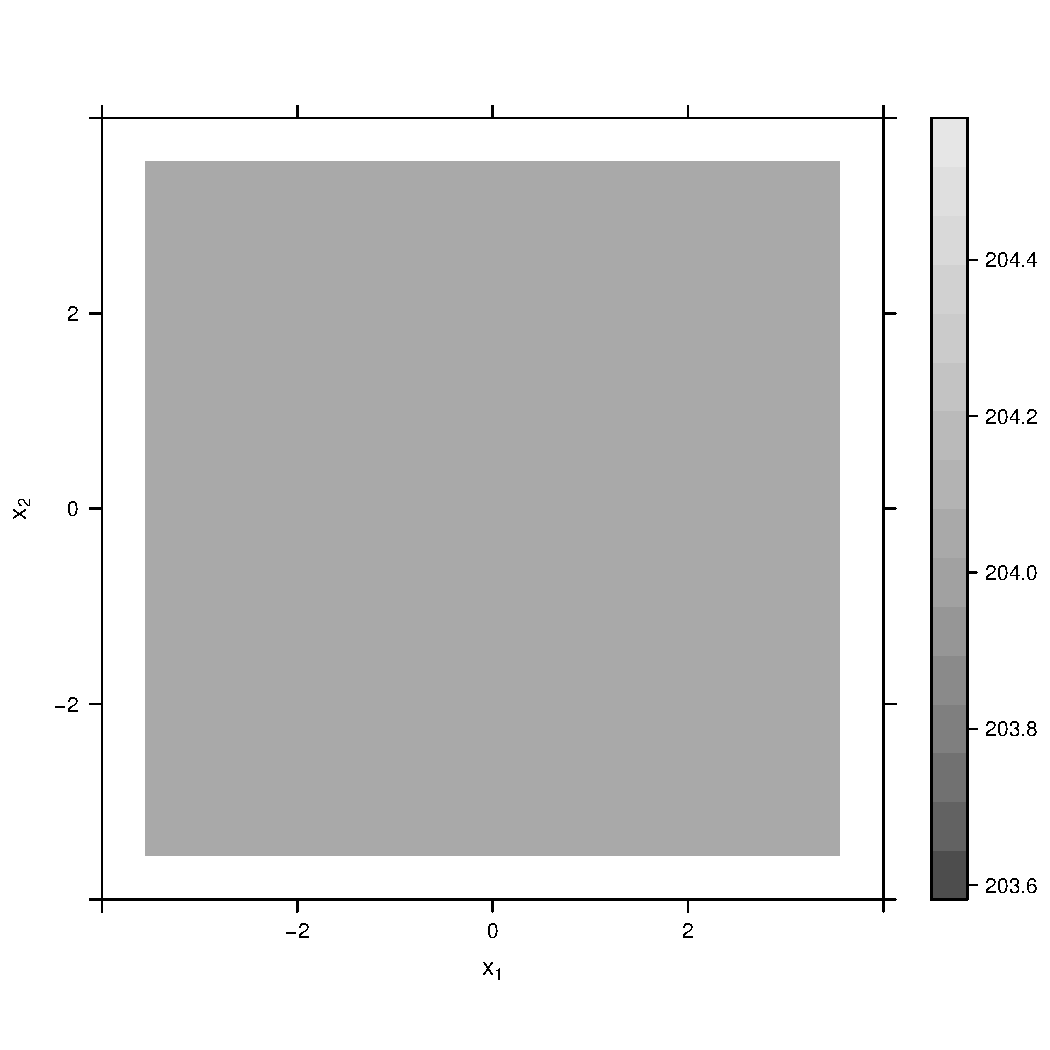
\includegraphics[width=\textwidth]{output/population-heatmap}
    \subcaption{Population distribution}
    \end{subfigure}
    \begin{subfigure}[t]{0.33\textwidth}
    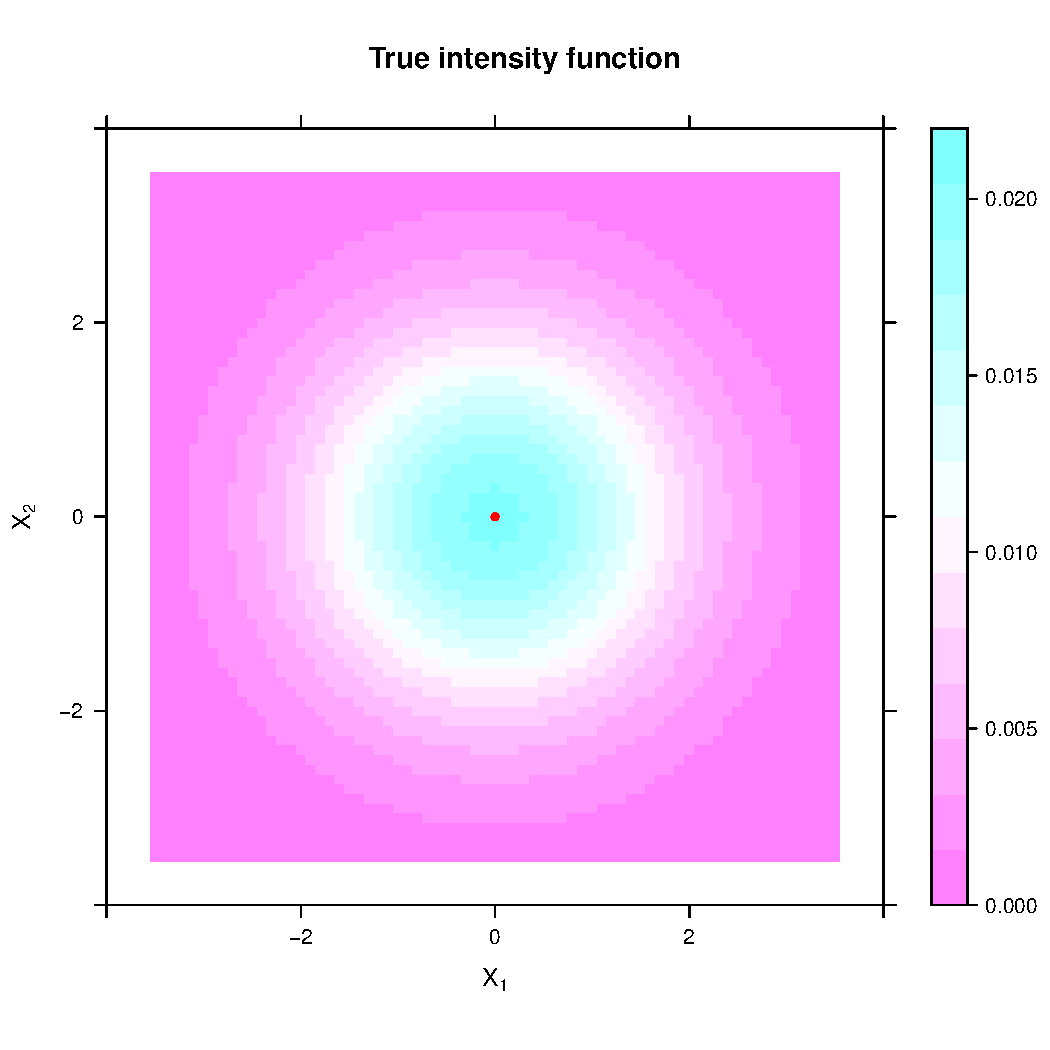
\includegraphics[width=\textwidth]{output/true_intensity_heatmap}
    \subcaption{True risk function}
    \end{subfigure}%
    \begin{subfigure}[t]{0.32\textwidth}
    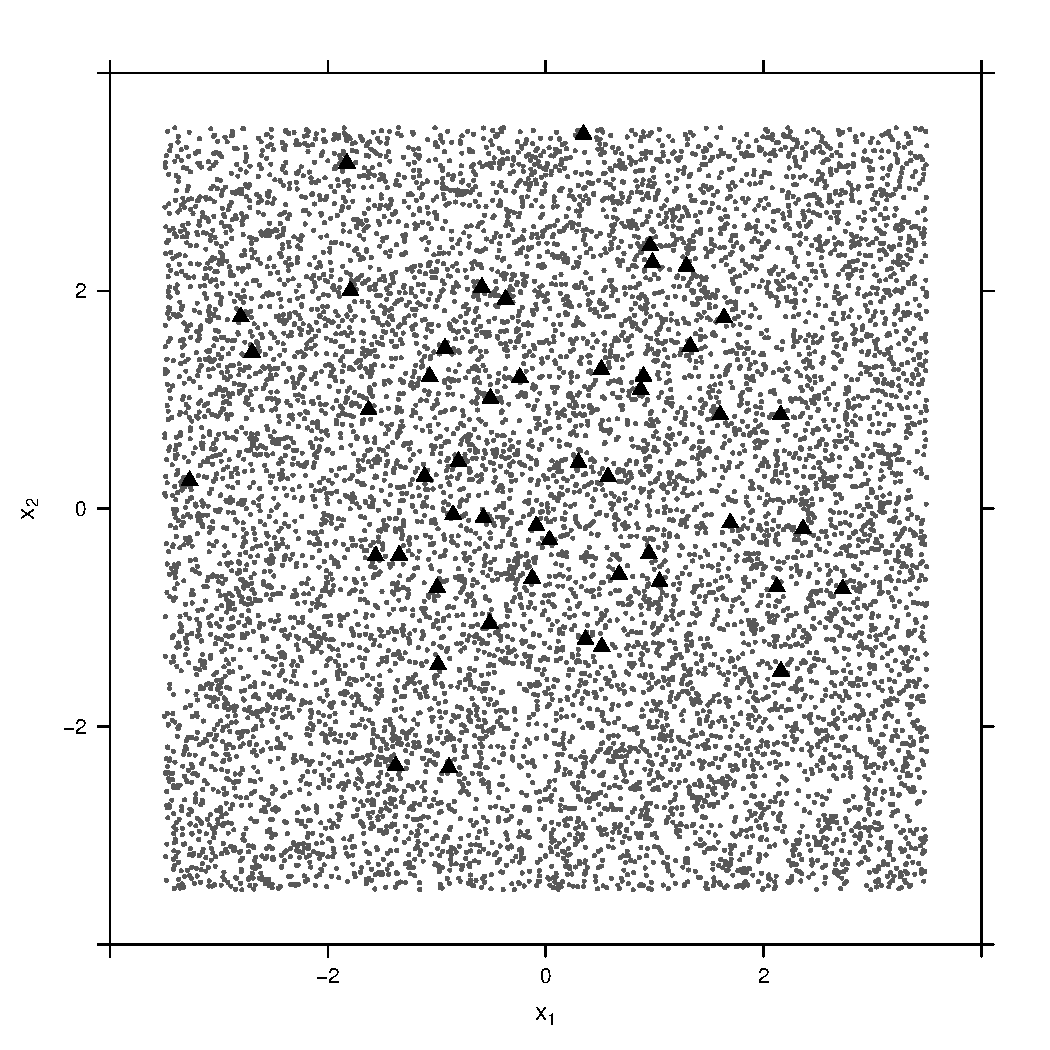
\includegraphics[width=\textwidth]{output/population_and_incidents_scatter}
    \subcaption{Population points (gray) with incidents (black)}
    \end{subfigure}%

    \caption[]{Population distribution (a), true risk function (b), and sample population with incidents (c) for uniform population of 10,000, single-peak risk of decay rate 1.4 and factor 50}
    \label{fig:distributions:unif_50_1.4_1h}    
\end{figure}


%%
%% Tables and figures for uniform population of 10,000, single-peak risk of decay rate 1.4, factor 100
%%
\graphicspath{{./results/unif_100_1.4_1h/}}
\makeatletter
\def\input@path{{./results/unif_100_1.4_1h/}}
\makeatother

\begin{table}[H]
    \centering
    \tiny
    \begin{subtable}[t]{0.5\textwidth}
        \centering
        \subcaption{Means} 
        % latex table generated in R 3.4.2 by xtable 1.8-2 package
% Sat Feb 17 16:44:44 2018
\begin{tabular}{lrrr}
  \hline
 & Oracle & Silverman & CV \\ 
  \hline
MISE & 0.000053 & 0.000083 & 0.000080 \\ 
  Relative MISE & 0.002028 & 0.003195 & 0.003047 \\ 
  Normalized MISE & 0.000026 & 0.000042 & 0.000040 \\ 
  MIAE & 0.003914 & 0.004863 & 0.004653 \\ 
  Relative MIAE & 0.024227 & 0.030102 & 0.028802 \\ 
  Max Error & 0.033855 & 0.049415 & 0.045884 \\ 
  Peak bias & -0.016050 & 0.010816 & -0.002953 \\ 
  Relative Peak bias & -0.099339 & 0.066949 & -0.018278 \\ 
  Peak drift & 0.223424 & 0.357624 & 0.284159 \\ 
  Relative Peak drift & 0.031918 & 0.051089 & 0.040594 \\ 
  Centroid bias & -0.017140 & -0.000902 & -0.013918 \\ 
  Relative Centroid bias & -0.106087 & -0.005583 & -0.086149 \\ 
  Centroid drift & 0.149249 & 0.159867 & 0.152694 \\ 
  Relative Centroid drift & 0.021321 & 0.022838 & 0.021813 \\ 
   \hline
\end{tabular}

    \end{subtable}%
    \begin{subtable}[t]{0.5\textwidth}
        \centering
        \subcaption{Standard deviations} 
        % latex table generated in R 3.4.3 by xtable 1.8-2 package
% Sun Apr 15 09:09:45 2018
\begin{tabular}{lrrr}
  \toprule
 & Oracle & Silverman & CV \\ 
  \midrule
MISE & 0.000014 & 0.000014 & 0.000021 \\ 
  Relative MISE & 0.001962 & 0.002039 & 0.003010 \\ 
  Normalized MISE & 0.344229 & 0.357804 & 0.528098 \\ 
  MIAE & 0.000689 & 0.000597 & 0.000961 \\ 
  Relative MIAE & 0.008228 & 0.007121 & 0.011473 \\ 
  Normalized MIAE & 0.000003 & 0.000003 & 0.000005 \\ 
  Supremum error & 0.005321 & 0.006343 & 0.008947 \\ 
  Normalized Sup error & 0.000027 & 0.000032 & 0.000045 \\ 
  Peak bias & 0.008408 & 0.012518 & 0.015040 \\ 
  Relative Peak bias & 0.100360 & 0.149419 & 0.179526 \\ 
  Peak drift & 0.186254 & 0.253752 & 0.225627 \\ 
  Relative Peak drift & 0.026608 & 0.036250 & 0.032232 \\ 
  Centroid bias & 0.008526 & 0.013326 & 0.013412 \\ 
  Relative Centroid bias & 0.101772 & 0.159063 & 0.160095 \\ 
  Centroid drift & 0.142123 & 0.159726 & 0.144847 \\ 
  Relative Centroid drift & 0.020303 & 0.022818 & 0.020692 \\ 
   \bottomrule
\end{tabular}

    \end{subtable}

\caption[]{Error rates for uniform population of 10,000, single-peak risk of decay rate 1.4 and factor 100}
\label{tab:mean_error_rates:unif_100_1.4_1h}
\end{table}

\begin{figure}[H]
        \centering
    \begin{subfigure}[t]{0.33\textwidth}
    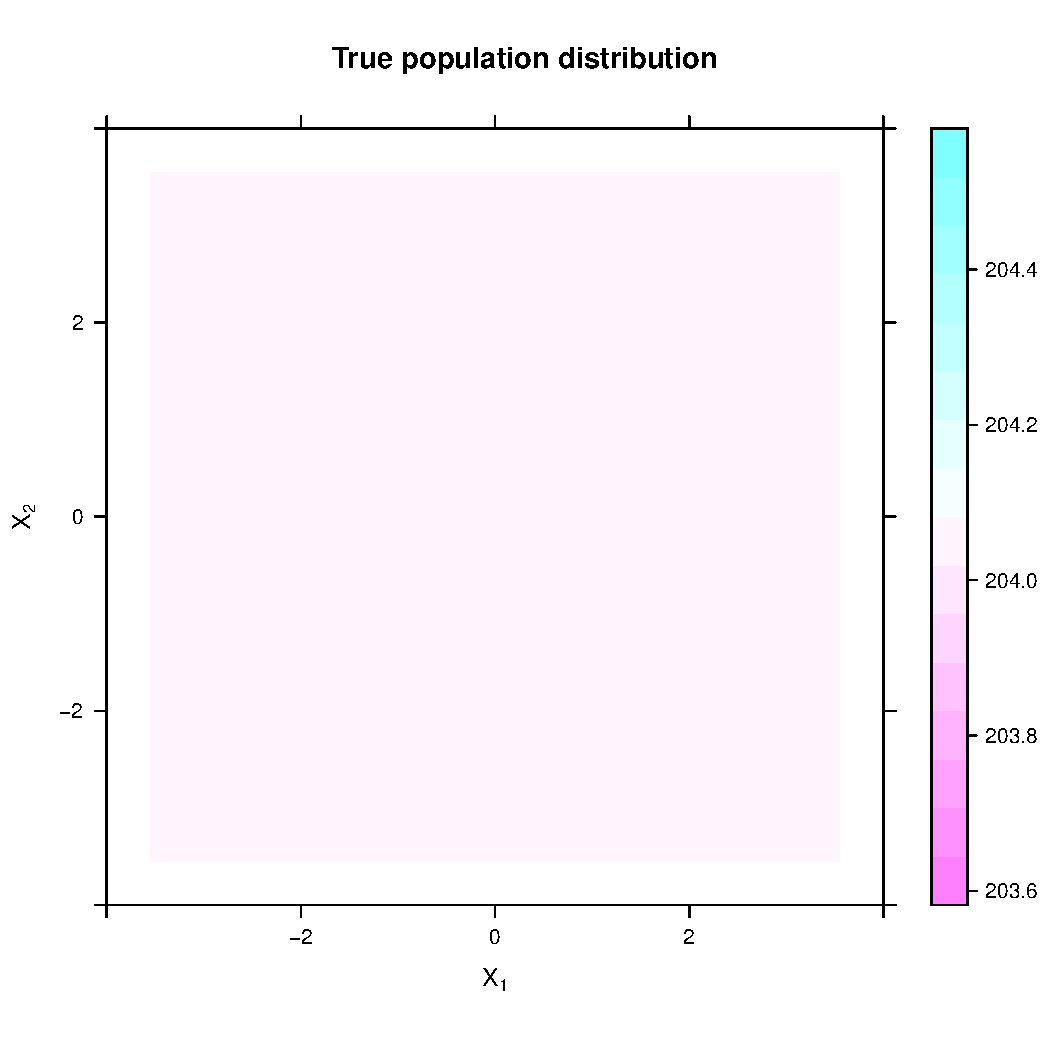
\includegraphics[width=\textwidth]{output/population-heatmap}
    \subcaption{Population distribution}
    \end{subfigure}
    \begin{subfigure}[t]{0.33\textwidth}
    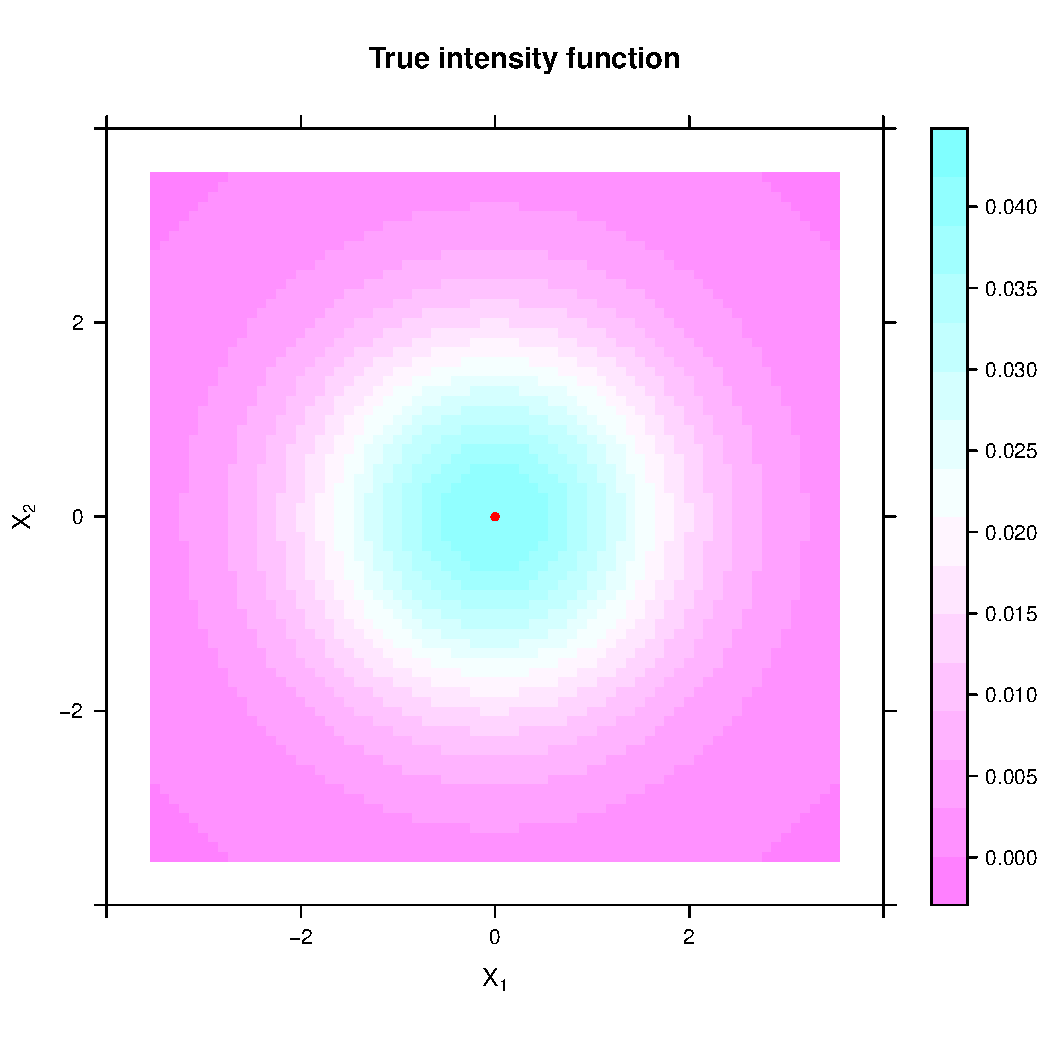
\includegraphics[width=\textwidth]{output/true_intensity_heatmap}
    \subcaption{True risk function}
    \end{subfigure}%
    \begin{subfigure}[t]{0.32\textwidth}
    \includegraphics[width=\textwidth]{output/population_and_incidents_scatter}
    \subcaption{Population points (gray) with incidents (black)}
    \end{subfigure}%

    \caption[]{Population distribution (a), true risk function (b), and sample population with incidents (c) for uniform population of 10,000, single-peak risk of decay rate 1.4 and factor 100}
    \label{fig:distributions:unif_100_1.4_1h}    
\end{figure}


%%
%% Tables and figures for uniform population of 10,000, single-peak risk of decay rate 1.4, factor 200
%%
\graphicspath{{./results/unif_200_1.4_1h/}}
\makeatletter
\def\input@path{{./results/unif_200_1.4_1h/}}
\makeatother

\begin{table}[H]
    \centering
    \tiny
    \begin{subtable}[t]{0.5\textwidth}
        \centering
        \subcaption{Means} 
        % latex table generated in R 3.4.2 by xtable 1.8-2 package
% Sat Feb 17 16:44:44 2018
\begin{tabular}{lrrr}
  \hline
 & Oracle & Silverman & CV \\ 
  \hline
MISE & 0.000053 & 0.000083 & 0.000080 \\ 
  Relative MISE & 0.002028 & 0.003195 & 0.003047 \\ 
  Normalized MISE & 0.000026 & 0.000042 & 0.000040 \\ 
  MIAE & 0.003914 & 0.004863 & 0.004653 \\ 
  Relative MIAE & 0.024227 & 0.030102 & 0.028802 \\ 
  Max Error & 0.033855 & 0.049415 & 0.045884 \\ 
  Peak bias & -0.016050 & 0.010816 & -0.002953 \\ 
  Relative Peak bias & -0.099339 & 0.066949 & -0.018278 \\ 
  Peak drift & 0.223424 & 0.357624 & 0.284159 \\ 
  Relative Peak drift & 0.031918 & 0.051089 & 0.040594 \\ 
  Centroid bias & -0.017140 & -0.000902 & -0.013918 \\ 
  Relative Centroid bias & -0.106087 & -0.005583 & -0.086149 \\ 
  Centroid drift & 0.149249 & 0.159867 & 0.152694 \\ 
  Relative Centroid drift & 0.021321 & 0.022838 & 0.021813 \\ 
   \hline
\end{tabular}

    \end{subtable}%
    \begin{subtable}[t]{0.5\textwidth}
        \centering
        \subcaption{Standard deviations} 
        % latex table generated in R 3.4.3 by xtable 1.8-2 package
% Sun Apr 15 09:09:45 2018
\begin{tabular}{lrrr}
  \toprule
 & Oracle & Silverman & CV \\ 
  \midrule
MISE & 0.000014 & 0.000014 & 0.000021 \\ 
  Relative MISE & 0.001962 & 0.002039 & 0.003010 \\ 
  Normalized MISE & 0.344229 & 0.357804 & 0.528098 \\ 
  MIAE & 0.000689 & 0.000597 & 0.000961 \\ 
  Relative MIAE & 0.008228 & 0.007121 & 0.011473 \\ 
  Normalized MIAE & 0.000003 & 0.000003 & 0.000005 \\ 
  Supremum error & 0.005321 & 0.006343 & 0.008947 \\ 
  Normalized Sup error & 0.000027 & 0.000032 & 0.000045 \\ 
  Peak bias & 0.008408 & 0.012518 & 0.015040 \\ 
  Relative Peak bias & 0.100360 & 0.149419 & 0.179526 \\ 
  Peak drift & 0.186254 & 0.253752 & 0.225627 \\ 
  Relative Peak drift & 0.026608 & 0.036250 & 0.032232 \\ 
  Centroid bias & 0.008526 & 0.013326 & 0.013412 \\ 
  Relative Centroid bias & 0.101772 & 0.159063 & 0.160095 \\ 
  Centroid drift & 0.142123 & 0.159726 & 0.144847 \\ 
  Relative Centroid drift & 0.020303 & 0.022818 & 0.020692 \\ 
   \bottomrule
\end{tabular}

    \end{subtable}

\caption[]{Error rates for uniform population of 10,000, single-peak risk of decay rate 1.4 and factor 200}
\label{tab:mean_error_rates:unif_200_1.4_1h}
\end{table}

\begin{figure}[H]
        \centering
    \begin{subfigure}[t]{0.33\textwidth}
    \includegraphics[width=\textwidth]{output/population-heatmap}
    \subcaption{Population distribution}
    \end{subfigure}
    \begin{subfigure}[t]{0.33\textwidth}
    \includegraphics[width=\textwidth]{output/true_intensity_heatmap}
    \subcaption{True risk function}
    \end{subfigure}%
    \begin{subfigure}[t]{0.32\textwidth}
    \includegraphics[width=\textwidth]{output/population_and_incidents_scatter}
    \subcaption{Population points (gray) with incidents (black)}
    \end{subfigure}%

    \caption[]{Population distribution (a), true risk function (b), and sample population with incidents (c) for uniform population of 10,000, single-peak risk of decay rate 1.4 and factor 200}
    \label{fig:distributions:unif_200_1.4_1h}    
\end{figure}


%%
%% Tables and figures for uniform population of 10,000, single-peak risk of decay rate 1.4, factor 500
%%
\graphicspath{{./results/unif_500_1.4_1h/}}
\makeatletter
\def\input@path{{./results/unif_500_1.4_1h/}}
\makeatother

\begin{table}[H]
    \centering
    \tiny
    \begin{subtable}[t]{0.5\textwidth}
        \centering
        \subcaption{Means} 
        % latex table generated in R 3.4.2 by xtable 1.8-2 package
% Sat Feb 17 16:44:44 2018
\begin{tabular}{lrrr}
  \hline
 & Oracle & Silverman & CV \\ 
  \hline
MISE & 0.000053 & 0.000083 & 0.000080 \\ 
  Relative MISE & 0.002028 & 0.003195 & 0.003047 \\ 
  Normalized MISE & 0.000026 & 0.000042 & 0.000040 \\ 
  MIAE & 0.003914 & 0.004863 & 0.004653 \\ 
  Relative MIAE & 0.024227 & 0.030102 & 0.028802 \\ 
  Max Error & 0.033855 & 0.049415 & 0.045884 \\ 
  Peak bias & -0.016050 & 0.010816 & -0.002953 \\ 
  Relative Peak bias & -0.099339 & 0.066949 & -0.018278 \\ 
  Peak drift & 0.223424 & 0.357624 & 0.284159 \\ 
  Relative Peak drift & 0.031918 & 0.051089 & 0.040594 \\ 
  Centroid bias & -0.017140 & -0.000902 & -0.013918 \\ 
  Relative Centroid bias & -0.106087 & -0.005583 & -0.086149 \\ 
  Centroid drift & 0.149249 & 0.159867 & 0.152694 \\ 
  Relative Centroid drift & 0.021321 & 0.022838 & 0.021813 \\ 
   \hline
\end{tabular}

    \end{subtable}%
    \begin{subtable}[t]{0.5\textwidth}
        \centering
        \subcaption{Standard deviations} 
        % latex table generated in R 3.4.3 by xtable 1.8-2 package
% Sun Apr 15 09:09:45 2018
\begin{tabular}{lrrr}
  \toprule
 & Oracle & Silverman & CV \\ 
  \midrule
MISE & 0.000014 & 0.000014 & 0.000021 \\ 
  Relative MISE & 0.001962 & 0.002039 & 0.003010 \\ 
  Normalized MISE & 0.344229 & 0.357804 & 0.528098 \\ 
  MIAE & 0.000689 & 0.000597 & 0.000961 \\ 
  Relative MIAE & 0.008228 & 0.007121 & 0.011473 \\ 
  Normalized MIAE & 0.000003 & 0.000003 & 0.000005 \\ 
  Supremum error & 0.005321 & 0.006343 & 0.008947 \\ 
  Normalized Sup error & 0.000027 & 0.000032 & 0.000045 \\ 
  Peak bias & 0.008408 & 0.012518 & 0.015040 \\ 
  Relative Peak bias & 0.100360 & 0.149419 & 0.179526 \\ 
  Peak drift & 0.186254 & 0.253752 & 0.225627 \\ 
  Relative Peak drift & 0.026608 & 0.036250 & 0.032232 \\ 
  Centroid bias & 0.008526 & 0.013326 & 0.013412 \\ 
  Relative Centroid bias & 0.101772 & 0.159063 & 0.160095 \\ 
  Centroid drift & 0.142123 & 0.159726 & 0.144847 \\ 
  Relative Centroid drift & 0.020303 & 0.022818 & 0.020692 \\ 
   \bottomrule
\end{tabular}

    \end{subtable}

\caption[]{Error rates for uniform population of 10,000, single-peak risk of decay rate 1.4 and factor 500}
\label{tab:mean_error_rates:unif_500_1.4_1h}
\end{table}

\begin{figure}[H]
        \centering
    \begin{subfigure}[t]{0.33\textwidth}
    \includegraphics[width=\textwidth]{output/population-heatmap}
    \subcaption{Population distribution}
    \end{subfigure}
    \begin{subfigure}[t]{0.33\textwidth}
    \includegraphics[width=\textwidth]{output/true_intensity_heatmap}
    \subcaption{True risk function}
    \end{subfigure}%
    \begin{subfigure}[t]{0.32\textwidth}
    \includegraphics[width=\textwidth]{output/population_and_incidents_scatter}
    \subcaption{Population points (gray) with incidents (black)}
    \end{subfigure}%

    \caption[]{Population distribution (a), true risk function (b), and sample population with incidents (c) for uniform population of 10,000, single-peak risk of decay rate 1.4 and factor 500}
    \label{fig:distributions:unif_500_1.4_1h}    
\end{figure}


%%
%% Tables and figures for uniform population of 10,000, single-peak risk of decay rate 1.4, factor 1,000
%%
\graphicspath{{./results/unif_1000_1.4_1h/}}
\makeatletter
\def\input@path{{./results/unif_1000_1.4_1h/}}
\makeatother

\begin{table}[H]
    \centering
    \tiny
    \begin{subtable}[t]{0.5\textwidth}
        \centering
        \subcaption{Means} 
        % latex table generated in R 3.4.2 by xtable 1.8-2 package
% Sat Feb 17 16:44:44 2018
\begin{tabular}{lrrr}
  \hline
 & Oracle & Silverman & CV \\ 
  \hline
MISE & 0.000053 & 0.000083 & 0.000080 \\ 
  Relative MISE & 0.002028 & 0.003195 & 0.003047 \\ 
  Normalized MISE & 0.000026 & 0.000042 & 0.000040 \\ 
  MIAE & 0.003914 & 0.004863 & 0.004653 \\ 
  Relative MIAE & 0.024227 & 0.030102 & 0.028802 \\ 
  Max Error & 0.033855 & 0.049415 & 0.045884 \\ 
  Peak bias & -0.016050 & 0.010816 & -0.002953 \\ 
  Relative Peak bias & -0.099339 & 0.066949 & -0.018278 \\ 
  Peak drift & 0.223424 & 0.357624 & 0.284159 \\ 
  Relative Peak drift & 0.031918 & 0.051089 & 0.040594 \\ 
  Centroid bias & -0.017140 & -0.000902 & -0.013918 \\ 
  Relative Centroid bias & -0.106087 & -0.005583 & -0.086149 \\ 
  Centroid drift & 0.149249 & 0.159867 & 0.152694 \\ 
  Relative Centroid drift & 0.021321 & 0.022838 & 0.021813 \\ 
   \hline
\end{tabular}

    \end{subtable}%
    \begin{subtable}[t]{0.5\textwidth}
        \centering
        \subcaption{Standard deviations} 
        % latex table generated in R 3.4.3 by xtable 1.8-2 package
% Sun Apr 15 09:09:45 2018
\begin{tabular}{lrrr}
  \toprule
 & Oracle & Silverman & CV \\ 
  \midrule
MISE & 0.000014 & 0.000014 & 0.000021 \\ 
  Relative MISE & 0.001962 & 0.002039 & 0.003010 \\ 
  Normalized MISE & 0.344229 & 0.357804 & 0.528098 \\ 
  MIAE & 0.000689 & 0.000597 & 0.000961 \\ 
  Relative MIAE & 0.008228 & 0.007121 & 0.011473 \\ 
  Normalized MIAE & 0.000003 & 0.000003 & 0.000005 \\ 
  Supremum error & 0.005321 & 0.006343 & 0.008947 \\ 
  Normalized Sup error & 0.000027 & 0.000032 & 0.000045 \\ 
  Peak bias & 0.008408 & 0.012518 & 0.015040 \\ 
  Relative Peak bias & 0.100360 & 0.149419 & 0.179526 \\ 
  Peak drift & 0.186254 & 0.253752 & 0.225627 \\ 
  Relative Peak drift & 0.026608 & 0.036250 & 0.032232 \\ 
  Centroid bias & 0.008526 & 0.013326 & 0.013412 \\ 
  Relative Centroid bias & 0.101772 & 0.159063 & 0.160095 \\ 
  Centroid drift & 0.142123 & 0.159726 & 0.144847 \\ 
  Relative Centroid drift & 0.020303 & 0.022818 & 0.020692 \\ 
   \bottomrule
\end{tabular}

    \end{subtable}

\caption[]{Error rates for uniform population of 10,000, single-peak risk of decay rate 1.4 and factor 1,000}
\label{tab:mean_error_rates:unif_1000_1.4_1h}
\end{table}

\begin{figure}[H]
        \centering
    \begin{subfigure}[t]{0.33\textwidth}
    \includegraphics[width=\textwidth]{output/population-heatmap}
    \subcaption{Population distribution}
    \end{subfigure}
    \begin{subfigure}[t]{0.33\textwidth}
    \includegraphics[width=\textwidth]{output/true_intensity_heatmap}
    \subcaption{True risk function}
    \end{subfigure}%
    \begin{subfigure}[t]{0.32\textwidth}
    \includegraphics[width=\textwidth]{output/population_and_incidents_scatter}
    \subcaption{Population points (gray) with incidents (black)}
    \end{subfigure}%

    \caption[]{Population distribution (a), true risk function (b), and sample population with incidents (c) for uniform population of 10,000, single-peak risk of decay rate 1.4 and factor 1,000}
    \label{fig:distributions:unif_1000_1.4_1h}    
\end{figure}

 
 
%%
%% Section containing single-peak risk with decay rate 2.0 on uniform population
%%
\section{Single-peak risk with decay rate 2.0 on a uniform population}
\label{sec:app:results_unif_2.0_1h}

%%
%% Tables and figures for uniform population of 10,000, single-peak risk of decay rate 2.0, factor 50
%%
\graphicspath{{./results/unif_50_2.0_1h/}}
\makeatletter
\def\input@path{{./results/unif_50_2.0_1h/}}
\makeatother

\begin{table}[H]
        \centering
    \tiny
    \begin{subtable}[t]{0.5\textwidth}
        \centering
        \subcaption{Means} 
        % latex table generated in R 3.4.2 by xtable 1.8-2 package
% Sat Feb 17 16:44:44 2018
\begin{tabular}{lrrr}
  \hline
 & Oracle & Silverman & CV \\ 
  \hline
MISE & 0.000053 & 0.000083 & 0.000080 \\ 
  Relative MISE & 0.002028 & 0.003195 & 0.003047 \\ 
  Normalized MISE & 0.000026 & 0.000042 & 0.000040 \\ 
  MIAE & 0.003914 & 0.004863 & 0.004653 \\ 
  Relative MIAE & 0.024227 & 0.030102 & 0.028802 \\ 
  Max Error & 0.033855 & 0.049415 & 0.045884 \\ 
  Peak bias & -0.016050 & 0.010816 & -0.002953 \\ 
  Relative Peak bias & -0.099339 & 0.066949 & -0.018278 \\ 
  Peak drift & 0.223424 & 0.357624 & 0.284159 \\ 
  Relative Peak drift & 0.031918 & 0.051089 & 0.040594 \\ 
  Centroid bias & -0.017140 & -0.000902 & -0.013918 \\ 
  Relative Centroid bias & -0.106087 & -0.005583 & -0.086149 \\ 
  Centroid drift & 0.149249 & 0.159867 & 0.152694 \\ 
  Relative Centroid drift & 0.021321 & 0.022838 & 0.021813 \\ 
   \hline
\end{tabular}

    \end{subtable}%
    \begin{subtable}[t]{0.5\textwidth}
        \centering
        \subcaption{Standard deviations} 
        % latex table generated in R 3.4.3 by xtable 1.8-2 package
% Sun Apr 15 09:09:45 2018
\begin{tabular}{lrrr}
  \toprule
 & Oracle & Silverman & CV \\ 
  \midrule
MISE & 0.000014 & 0.000014 & 0.000021 \\ 
  Relative MISE & 0.001962 & 0.002039 & 0.003010 \\ 
  Normalized MISE & 0.344229 & 0.357804 & 0.528098 \\ 
  MIAE & 0.000689 & 0.000597 & 0.000961 \\ 
  Relative MIAE & 0.008228 & 0.007121 & 0.011473 \\ 
  Normalized MIAE & 0.000003 & 0.000003 & 0.000005 \\ 
  Supremum error & 0.005321 & 0.006343 & 0.008947 \\ 
  Normalized Sup error & 0.000027 & 0.000032 & 0.000045 \\ 
  Peak bias & 0.008408 & 0.012518 & 0.015040 \\ 
  Relative Peak bias & 0.100360 & 0.149419 & 0.179526 \\ 
  Peak drift & 0.186254 & 0.253752 & 0.225627 \\ 
  Relative Peak drift & 0.026608 & 0.036250 & 0.032232 \\ 
  Centroid bias & 0.008526 & 0.013326 & 0.013412 \\ 
  Relative Centroid bias & 0.101772 & 0.159063 & 0.160095 \\ 
  Centroid drift & 0.142123 & 0.159726 & 0.144847 \\ 
  Relative Centroid drift & 0.020303 & 0.022818 & 0.020692 \\ 
   \bottomrule
\end{tabular}

    \end{subtable}

    \caption[]{Error rates for uniform population of 10,000, single-peak risk of decay rate 2.0 and factor 50}
    \label{tab:mean_error_rates:unif_50_2.0_1h}
\end{table}

\begin{figure}[H]
        \centering
    \begin{subfigure}[t]{0.33\textwidth}
    \includegraphics[width=\textwidth]{output/population-heatmap}
    \subcaption{Population distribution}
    \end{subfigure}
    \begin{subfigure}[t]{0.33\textwidth}
    \includegraphics[width=\textwidth]{output/true_intensity_heatmap}
    \subcaption{True risk function}
    \end{subfigure}%
    \begin{subfigure}[t]{0.32\textwidth}
    \includegraphics[width=\textwidth]{output/population_and_incidents_scatter}
    \subcaption{Population points (gray) with incidents (black)}
    \end{subfigure}%

    \caption[]{Population distribution (a), true risk function (b), and sample population with incidents (c) for uniform population of 10,000, single-peak risk of decay rate 2.0 and factor 50}
    \label{fig:distributions:unif_50_2.0_1h}    
\end{figure}


%%
%% Tables and figures for uniform population of 10,000, single-peak risk of decay rate 2.0, factor 100
%%
\graphicspath{{./results/unif_100_2.0_1h/}}
\makeatletter
\def\input@path{{./results/unif_100_2.0_1h/}}
\makeatother

\begin{table}[H]
    \centering
    \tiny
    \begin{subtable}[t]{0.5\textwidth}
        \centering
        \subcaption{Means} 
        % latex table generated in R 3.4.2 by xtable 1.8-2 package
% Sat Feb 17 16:44:44 2018
\begin{tabular}{lrrr}
  \hline
 & Oracle & Silverman & CV \\ 
  \hline
MISE & 0.000053 & 0.000083 & 0.000080 \\ 
  Relative MISE & 0.002028 & 0.003195 & 0.003047 \\ 
  Normalized MISE & 0.000026 & 0.000042 & 0.000040 \\ 
  MIAE & 0.003914 & 0.004863 & 0.004653 \\ 
  Relative MIAE & 0.024227 & 0.030102 & 0.028802 \\ 
  Max Error & 0.033855 & 0.049415 & 0.045884 \\ 
  Peak bias & -0.016050 & 0.010816 & -0.002953 \\ 
  Relative Peak bias & -0.099339 & 0.066949 & -0.018278 \\ 
  Peak drift & 0.223424 & 0.357624 & 0.284159 \\ 
  Relative Peak drift & 0.031918 & 0.051089 & 0.040594 \\ 
  Centroid bias & -0.017140 & -0.000902 & -0.013918 \\ 
  Relative Centroid bias & -0.106087 & -0.005583 & -0.086149 \\ 
  Centroid drift & 0.149249 & 0.159867 & 0.152694 \\ 
  Relative Centroid drift & 0.021321 & 0.022838 & 0.021813 \\ 
   \hline
\end{tabular}

    \end{subtable}%
    \begin{subtable}[t]{0.5\textwidth}
        \centering
        \subcaption{Standard deviations} 
        % latex table generated in R 3.4.3 by xtable 1.8-2 package
% Sun Apr 15 09:09:45 2018
\begin{tabular}{lrrr}
  \toprule
 & Oracle & Silverman & CV \\ 
  \midrule
MISE & 0.000014 & 0.000014 & 0.000021 \\ 
  Relative MISE & 0.001962 & 0.002039 & 0.003010 \\ 
  Normalized MISE & 0.344229 & 0.357804 & 0.528098 \\ 
  MIAE & 0.000689 & 0.000597 & 0.000961 \\ 
  Relative MIAE & 0.008228 & 0.007121 & 0.011473 \\ 
  Normalized MIAE & 0.000003 & 0.000003 & 0.000005 \\ 
  Supremum error & 0.005321 & 0.006343 & 0.008947 \\ 
  Normalized Sup error & 0.000027 & 0.000032 & 0.000045 \\ 
  Peak bias & 0.008408 & 0.012518 & 0.015040 \\ 
  Relative Peak bias & 0.100360 & 0.149419 & 0.179526 \\ 
  Peak drift & 0.186254 & 0.253752 & 0.225627 \\ 
  Relative Peak drift & 0.026608 & 0.036250 & 0.032232 \\ 
  Centroid bias & 0.008526 & 0.013326 & 0.013412 \\ 
  Relative Centroid bias & 0.101772 & 0.159063 & 0.160095 \\ 
  Centroid drift & 0.142123 & 0.159726 & 0.144847 \\ 
  Relative Centroid drift & 0.020303 & 0.022818 & 0.020692 \\ 
   \bottomrule
\end{tabular}

    \end{subtable}

\caption[]{Error rates for uniform population of 10,000, single-peak risk of decay rate 2.0 and factor 100}
\label{tab:mean_error_rates:unif_100_2.0_1h}
\end{table}

\begin{figure}[H]
        \centering
    \begin{subfigure}[t]{0.33\textwidth}
    \includegraphics[width=\textwidth]{output/population-heatmap}
    \subcaption{Population distribution}
    \end{subfigure}
    \begin{subfigure}[t]{0.33\textwidth}
    \includegraphics[width=\textwidth]{output/true_intensity_heatmap}
    \subcaption{True risk function}
    \end{subfigure}%
    \begin{subfigure}[t]{0.32\textwidth}
    \includegraphics[width=\textwidth]{output/population_and_incidents_scatter}
    \subcaption{Population points (gray) with incidents (black)}
    \end{subfigure}%

    \caption[]{Population distribution (a), true risk function (b), and sample population with incidents (c) for uniform population of 10,000, single-peak risk of decay rate 2.0 and factor 100}
    \label{fig:distributions:unif_100_2.0_1h}    
\end{figure}


%%
%% Tables and figures for uniform population of 10,000, single-peak risk of decay rate 2.0, factor 200
%%
\graphicspath{{./results/unif_200_2.0_1h/}}
\makeatletter
\def\input@path{{./results/unif_200_2.0_1h/}}
\makeatother

\begin{table}[H]
    \centering
    \tiny
    \begin{subtable}[t]{0.5\textwidth}
        \centering
        \subcaption{Means} 
        % latex table generated in R 3.4.2 by xtable 1.8-2 package
% Sat Feb 17 16:44:44 2018
\begin{tabular}{lrrr}
  \hline
 & Oracle & Silverman & CV \\ 
  \hline
MISE & 0.000053 & 0.000083 & 0.000080 \\ 
  Relative MISE & 0.002028 & 0.003195 & 0.003047 \\ 
  Normalized MISE & 0.000026 & 0.000042 & 0.000040 \\ 
  MIAE & 0.003914 & 0.004863 & 0.004653 \\ 
  Relative MIAE & 0.024227 & 0.030102 & 0.028802 \\ 
  Max Error & 0.033855 & 0.049415 & 0.045884 \\ 
  Peak bias & -0.016050 & 0.010816 & -0.002953 \\ 
  Relative Peak bias & -0.099339 & 0.066949 & -0.018278 \\ 
  Peak drift & 0.223424 & 0.357624 & 0.284159 \\ 
  Relative Peak drift & 0.031918 & 0.051089 & 0.040594 \\ 
  Centroid bias & -0.017140 & -0.000902 & -0.013918 \\ 
  Relative Centroid bias & -0.106087 & -0.005583 & -0.086149 \\ 
  Centroid drift & 0.149249 & 0.159867 & 0.152694 \\ 
  Relative Centroid drift & 0.021321 & 0.022838 & 0.021813 \\ 
   \hline
\end{tabular}

    \end{subtable}%
    \begin{subtable}[t]{0.5\textwidth}
        \centering
        \subcaption{Standard deviations} 
        % latex table generated in R 3.4.3 by xtable 1.8-2 package
% Sun Apr 15 09:09:45 2018
\begin{tabular}{lrrr}
  \toprule
 & Oracle & Silverman & CV \\ 
  \midrule
MISE & 0.000014 & 0.000014 & 0.000021 \\ 
  Relative MISE & 0.001962 & 0.002039 & 0.003010 \\ 
  Normalized MISE & 0.344229 & 0.357804 & 0.528098 \\ 
  MIAE & 0.000689 & 0.000597 & 0.000961 \\ 
  Relative MIAE & 0.008228 & 0.007121 & 0.011473 \\ 
  Normalized MIAE & 0.000003 & 0.000003 & 0.000005 \\ 
  Supremum error & 0.005321 & 0.006343 & 0.008947 \\ 
  Normalized Sup error & 0.000027 & 0.000032 & 0.000045 \\ 
  Peak bias & 0.008408 & 0.012518 & 0.015040 \\ 
  Relative Peak bias & 0.100360 & 0.149419 & 0.179526 \\ 
  Peak drift & 0.186254 & 0.253752 & 0.225627 \\ 
  Relative Peak drift & 0.026608 & 0.036250 & 0.032232 \\ 
  Centroid bias & 0.008526 & 0.013326 & 0.013412 \\ 
  Relative Centroid bias & 0.101772 & 0.159063 & 0.160095 \\ 
  Centroid drift & 0.142123 & 0.159726 & 0.144847 \\ 
  Relative Centroid drift & 0.020303 & 0.022818 & 0.020692 \\ 
   \bottomrule
\end{tabular}

    \end{subtable}

\caption[]{Error rates for uniform population of 10,000, single-peak risk of decay rate 2.0 and factor 200}
\label{tab:mean_error_rates:unif_200_2.0_1h}
\end{table}

\begin{figure}[H]
        \centering
    \begin{subfigure}[t]{0.33\textwidth}
    \includegraphics[width=\textwidth]{output/population-heatmap}
    \subcaption{Population distribution}
    \end{subfigure}
    \begin{subfigure}[t]{0.33\textwidth}
    \includegraphics[width=\textwidth]{output/true_intensity_heatmap}
    \subcaption{True risk function}
    \end{subfigure}%
    \begin{subfigure}[t]{0.32\textwidth}
    \includegraphics[width=\textwidth]{output/population_and_incidents_scatter}
    \subcaption{Population points (gray) with incidents (black)}
    \end{subfigure}%

    \caption[]{Population distribution (a), true risk function (b), and sample population with incidents (c) for uniform population of 10,000, single-peak risk of decay rate 2.0 and factor 200}
    \label{fig:distributions:unif_200_2.0_1h}    
\end{figure}


%%
%% Tables and figures for uniform population of 10,000, single-peak risk of decay rate 2.0, factor 500
%%
\graphicspath{{./results/unif_500_2.0_1h/}}
\makeatletter
\def\input@path{{./results/unif_500_2.0_1h/}}
\makeatother

\begin{table}[H]
    \centering
    \tiny
    \begin{subtable}[t]{0.5\textwidth}
        \centering
        \subcaption{Means} 
        % latex table generated in R 3.4.2 by xtable 1.8-2 package
% Sat Feb 17 16:44:44 2018
\begin{tabular}{lrrr}
  \hline
 & Oracle & Silverman & CV \\ 
  \hline
MISE & 0.000053 & 0.000083 & 0.000080 \\ 
  Relative MISE & 0.002028 & 0.003195 & 0.003047 \\ 
  Normalized MISE & 0.000026 & 0.000042 & 0.000040 \\ 
  MIAE & 0.003914 & 0.004863 & 0.004653 \\ 
  Relative MIAE & 0.024227 & 0.030102 & 0.028802 \\ 
  Max Error & 0.033855 & 0.049415 & 0.045884 \\ 
  Peak bias & -0.016050 & 0.010816 & -0.002953 \\ 
  Relative Peak bias & -0.099339 & 0.066949 & -0.018278 \\ 
  Peak drift & 0.223424 & 0.357624 & 0.284159 \\ 
  Relative Peak drift & 0.031918 & 0.051089 & 0.040594 \\ 
  Centroid bias & -0.017140 & -0.000902 & -0.013918 \\ 
  Relative Centroid bias & -0.106087 & -0.005583 & -0.086149 \\ 
  Centroid drift & 0.149249 & 0.159867 & 0.152694 \\ 
  Relative Centroid drift & 0.021321 & 0.022838 & 0.021813 \\ 
   \hline
\end{tabular}

    \end{subtable}%
    \begin{subtable}[t]{0.5\textwidth}
        \centering
        \subcaption{Standard deviations} 
        % latex table generated in R 3.4.3 by xtable 1.8-2 package
% Sun Apr 15 09:09:45 2018
\begin{tabular}{lrrr}
  \toprule
 & Oracle & Silverman & CV \\ 
  \midrule
MISE & 0.000014 & 0.000014 & 0.000021 \\ 
  Relative MISE & 0.001962 & 0.002039 & 0.003010 \\ 
  Normalized MISE & 0.344229 & 0.357804 & 0.528098 \\ 
  MIAE & 0.000689 & 0.000597 & 0.000961 \\ 
  Relative MIAE & 0.008228 & 0.007121 & 0.011473 \\ 
  Normalized MIAE & 0.000003 & 0.000003 & 0.000005 \\ 
  Supremum error & 0.005321 & 0.006343 & 0.008947 \\ 
  Normalized Sup error & 0.000027 & 0.000032 & 0.000045 \\ 
  Peak bias & 0.008408 & 0.012518 & 0.015040 \\ 
  Relative Peak bias & 0.100360 & 0.149419 & 0.179526 \\ 
  Peak drift & 0.186254 & 0.253752 & 0.225627 \\ 
  Relative Peak drift & 0.026608 & 0.036250 & 0.032232 \\ 
  Centroid bias & 0.008526 & 0.013326 & 0.013412 \\ 
  Relative Centroid bias & 0.101772 & 0.159063 & 0.160095 \\ 
  Centroid drift & 0.142123 & 0.159726 & 0.144847 \\ 
  Relative Centroid drift & 0.020303 & 0.022818 & 0.020692 \\ 
   \bottomrule
\end{tabular}

    \end{subtable}

\caption[]{Error rates for uniform population of 10,000, single-peak risk of decay rate 2.0 and factor 500}
\label{tab:mean_error_rates:unif_500_2.0_1h}
\end{table}

\begin{figure}[H]
        \centering
    \begin{subfigure}[t]{0.33\textwidth}
    \includegraphics[width=\textwidth]{output/population-heatmap}
    \subcaption{Population distribution}
    \end{subfigure}
    \begin{subfigure}[t]{0.33\textwidth}
    \includegraphics[width=\textwidth]{output/true_intensity_heatmap}
    \subcaption{True risk function}
    \end{subfigure}%
    \begin{subfigure}[t]{0.32\textwidth}
    \includegraphics[width=\textwidth]{output/population_and_incidents_scatter}
    \subcaption{Population points (gray) with incidents (black)}
    \end{subfigure}%

    \caption[]{Population distribution (a), true risk function (b), and sample population with incidents (c) for uniform population of 10,000, single-peak risk of decay rate 2.0 and factor 500}
    \label{fig:distributions:unif_500_2.0_1h}    
\end{figure}


%%
%% Tables and figures for uniform population of 10,000, single-peak risk of decay rate 2.0, factor 1,000
%%
\graphicspath{{./results/unif_1000_2.0_1h/}}
\makeatletter
\def\input@path{{./results/unif_1000_2.0_1h/}}
\makeatother

\begin{table}[H]
    \centering
    \tiny
    \begin{subtable}[t]{0.5\textwidth}
        \centering
        \subcaption{Means} 
        % latex table generated in R 3.4.2 by xtable 1.8-2 package
% Sat Feb 17 16:44:44 2018
\begin{tabular}{lrrr}
  \hline
 & Oracle & Silverman & CV \\ 
  \hline
MISE & 0.000053 & 0.000083 & 0.000080 \\ 
  Relative MISE & 0.002028 & 0.003195 & 0.003047 \\ 
  Normalized MISE & 0.000026 & 0.000042 & 0.000040 \\ 
  MIAE & 0.003914 & 0.004863 & 0.004653 \\ 
  Relative MIAE & 0.024227 & 0.030102 & 0.028802 \\ 
  Max Error & 0.033855 & 0.049415 & 0.045884 \\ 
  Peak bias & -0.016050 & 0.010816 & -0.002953 \\ 
  Relative Peak bias & -0.099339 & 0.066949 & -0.018278 \\ 
  Peak drift & 0.223424 & 0.357624 & 0.284159 \\ 
  Relative Peak drift & 0.031918 & 0.051089 & 0.040594 \\ 
  Centroid bias & -0.017140 & -0.000902 & -0.013918 \\ 
  Relative Centroid bias & -0.106087 & -0.005583 & -0.086149 \\ 
  Centroid drift & 0.149249 & 0.159867 & 0.152694 \\ 
  Relative Centroid drift & 0.021321 & 0.022838 & 0.021813 \\ 
   \hline
\end{tabular}

    \end{subtable}%
    \begin{subtable}[t]{0.5\textwidth}
        \centering
        \subcaption{Standard deviations} 
        % latex table generated in R 3.4.3 by xtable 1.8-2 package
% Sun Apr 15 09:09:45 2018
\begin{tabular}{lrrr}
  \toprule
 & Oracle & Silverman & CV \\ 
  \midrule
MISE & 0.000014 & 0.000014 & 0.000021 \\ 
  Relative MISE & 0.001962 & 0.002039 & 0.003010 \\ 
  Normalized MISE & 0.344229 & 0.357804 & 0.528098 \\ 
  MIAE & 0.000689 & 0.000597 & 0.000961 \\ 
  Relative MIAE & 0.008228 & 0.007121 & 0.011473 \\ 
  Normalized MIAE & 0.000003 & 0.000003 & 0.000005 \\ 
  Supremum error & 0.005321 & 0.006343 & 0.008947 \\ 
  Normalized Sup error & 0.000027 & 0.000032 & 0.000045 \\ 
  Peak bias & 0.008408 & 0.012518 & 0.015040 \\ 
  Relative Peak bias & 0.100360 & 0.149419 & 0.179526 \\ 
  Peak drift & 0.186254 & 0.253752 & 0.225627 \\ 
  Relative Peak drift & 0.026608 & 0.036250 & 0.032232 \\ 
  Centroid bias & 0.008526 & 0.013326 & 0.013412 \\ 
  Relative Centroid bias & 0.101772 & 0.159063 & 0.160095 \\ 
  Centroid drift & 0.142123 & 0.159726 & 0.144847 \\ 
  Relative Centroid drift & 0.020303 & 0.022818 & 0.020692 \\ 
   \bottomrule
\end{tabular}

    \end{subtable}

\caption[]{Error rates for uniform population of 10,000, single-peak risk of decay rate 2.0 and factor 1,000}
\label{tab:mean_error_rates:unif_1000_2.0_1h}
\end{table}

\begin{figure}[H]
        \centering
    \begin{subfigure}[t]{0.33\textwidth}
    \includegraphics[width=\textwidth]{output/population-heatmap}
    \subcaption{Population distribution}
    \end{subfigure}
    \begin{subfigure}[t]{0.33\textwidth}
    \includegraphics[width=\textwidth]{output/true_intensity_heatmap}
    \subcaption{True risk function}
    \end{subfigure}%
    \begin{subfigure}[t]{0.32\textwidth}
    \includegraphics[width=\textwidth]{output/population_and_incidents_scatter}
    \subcaption{Population points (gray) with incidents (black)}
    \end{subfigure}%

    \caption[]{Population distribution (a), true risk function (b), and sample population with incidents (c) for uniform population of 10,000, single-peak risk of decay rate 2.0 and factor 1,000}
    \label{fig:distributions:unif_1000_2.0_1h}    
\end{figure}


 
%%
%% Section containing single-peak risk with decay rate 2.8 on uniform population
%%
\section{Single-peak risk with decay rate 2.8 on a uniform population}
\label{sec:app:results_unif_2.8_1h}

%%
%% Tables and figures for uniform population of 10,000, single-peak risk of decay rate 2.8, factor 50
%%
\graphicspath{{./results/unif_50_2.8_1h/}}
\makeatletter
\def\input@path{{./results/unif_50_2.8_1h/}}
\makeatother

\begin{table}[H]
        \centering
    \tiny
    \begin{subtable}[t]{0.5\textwidth}
        \centering
        \subcaption{Means} 
        % latex table generated in R 3.4.2 by xtable 1.8-2 package
% Sat Feb 17 16:44:44 2018
\begin{tabular}{lrrr}
  \hline
 & Oracle & Silverman & CV \\ 
  \hline
MISE & 0.000053 & 0.000083 & 0.000080 \\ 
  Relative MISE & 0.002028 & 0.003195 & 0.003047 \\ 
  Normalized MISE & 0.000026 & 0.000042 & 0.000040 \\ 
  MIAE & 0.003914 & 0.004863 & 0.004653 \\ 
  Relative MIAE & 0.024227 & 0.030102 & 0.028802 \\ 
  Max Error & 0.033855 & 0.049415 & 0.045884 \\ 
  Peak bias & -0.016050 & 0.010816 & -0.002953 \\ 
  Relative Peak bias & -0.099339 & 0.066949 & -0.018278 \\ 
  Peak drift & 0.223424 & 0.357624 & 0.284159 \\ 
  Relative Peak drift & 0.031918 & 0.051089 & 0.040594 \\ 
  Centroid bias & -0.017140 & -0.000902 & -0.013918 \\ 
  Relative Centroid bias & -0.106087 & -0.005583 & -0.086149 \\ 
  Centroid drift & 0.149249 & 0.159867 & 0.152694 \\ 
  Relative Centroid drift & 0.021321 & 0.022838 & 0.021813 \\ 
   \hline
\end{tabular}

    \end{subtable}%
    \begin{subtable}[t]{0.5\textwidth}
        \centering
        \subcaption{Standard deviations} 
        % latex table generated in R 3.4.3 by xtable 1.8-2 package
% Sun Apr 15 09:09:45 2018
\begin{tabular}{lrrr}
  \toprule
 & Oracle & Silverman & CV \\ 
  \midrule
MISE & 0.000014 & 0.000014 & 0.000021 \\ 
  Relative MISE & 0.001962 & 0.002039 & 0.003010 \\ 
  Normalized MISE & 0.344229 & 0.357804 & 0.528098 \\ 
  MIAE & 0.000689 & 0.000597 & 0.000961 \\ 
  Relative MIAE & 0.008228 & 0.007121 & 0.011473 \\ 
  Normalized MIAE & 0.000003 & 0.000003 & 0.000005 \\ 
  Supremum error & 0.005321 & 0.006343 & 0.008947 \\ 
  Normalized Sup error & 0.000027 & 0.000032 & 0.000045 \\ 
  Peak bias & 0.008408 & 0.012518 & 0.015040 \\ 
  Relative Peak bias & 0.100360 & 0.149419 & 0.179526 \\ 
  Peak drift & 0.186254 & 0.253752 & 0.225627 \\ 
  Relative Peak drift & 0.026608 & 0.036250 & 0.032232 \\ 
  Centroid bias & 0.008526 & 0.013326 & 0.013412 \\ 
  Relative Centroid bias & 0.101772 & 0.159063 & 0.160095 \\ 
  Centroid drift & 0.142123 & 0.159726 & 0.144847 \\ 
  Relative Centroid drift & 0.020303 & 0.022818 & 0.020692 \\ 
   \bottomrule
\end{tabular}

    \end{subtable}

    \caption[]{Error rates for uniform population of 10,000, single-peak risk of decay rate 2.8 and factor 50}
    \label{tab:mean_error_rates:unif_50_2.8_1h}
\end{table}

\begin{figure}[H]
        \centering
    \begin{subfigure}[t]{0.33\textwidth}
    \includegraphics[width=\textwidth]{output/population-heatmap}
    \subcaption{Population distribution}
    \end{subfigure}
    \begin{subfigure}[t]{0.33\textwidth}
    \includegraphics[width=\textwidth]{output/true_intensity_heatmap}
    \subcaption{True risk function}
    \end{subfigure}%
    \begin{subfigure}[t]{0.32\textwidth}
    \includegraphics[width=\textwidth]{output/population_and_incidents_scatter}
    \subcaption{Population points (gray) with incidents (black)}
    \end{subfigure}%

    \caption[]{Population distribution (a), true risk function (b), and sample population with incidents (c) for uniform population of 10,000, single-peak risk of decay rate 2.8 and factor 50}
    \label{fig:distributions:unif_50_2.8_1h}    
\end{figure}


%%
%% Tables and figures for uniform population of 10,000, single-peak risk of decay rate 2.8, factor 100
%%
\graphicspath{{./results/unif_100_2.8_1h/}}
\makeatletter
\def\input@path{{./results/unif_100_2.8_1h/}}
\makeatother

\begin{table}[H]
    \centering
    \tiny
    \begin{subtable}[t]{0.5\textwidth}
        \centering
        \subcaption{Means} 
        % latex table generated in R 3.4.2 by xtable 1.8-2 package
% Sat Feb 17 16:44:44 2018
\begin{tabular}{lrrr}
  \hline
 & Oracle & Silverman & CV \\ 
  \hline
MISE & 0.000053 & 0.000083 & 0.000080 \\ 
  Relative MISE & 0.002028 & 0.003195 & 0.003047 \\ 
  Normalized MISE & 0.000026 & 0.000042 & 0.000040 \\ 
  MIAE & 0.003914 & 0.004863 & 0.004653 \\ 
  Relative MIAE & 0.024227 & 0.030102 & 0.028802 \\ 
  Max Error & 0.033855 & 0.049415 & 0.045884 \\ 
  Peak bias & -0.016050 & 0.010816 & -0.002953 \\ 
  Relative Peak bias & -0.099339 & 0.066949 & -0.018278 \\ 
  Peak drift & 0.223424 & 0.357624 & 0.284159 \\ 
  Relative Peak drift & 0.031918 & 0.051089 & 0.040594 \\ 
  Centroid bias & -0.017140 & -0.000902 & -0.013918 \\ 
  Relative Centroid bias & -0.106087 & -0.005583 & -0.086149 \\ 
  Centroid drift & 0.149249 & 0.159867 & 0.152694 \\ 
  Relative Centroid drift & 0.021321 & 0.022838 & 0.021813 \\ 
   \hline
\end{tabular}

    \end{subtable}%
    \begin{subtable}[t]{0.5\textwidth}
        \centering
        \subcaption{Standard deviations} 
        % latex table generated in R 3.4.3 by xtable 1.8-2 package
% Sun Apr 15 09:09:45 2018
\begin{tabular}{lrrr}
  \toprule
 & Oracle & Silverman & CV \\ 
  \midrule
MISE & 0.000014 & 0.000014 & 0.000021 \\ 
  Relative MISE & 0.001962 & 0.002039 & 0.003010 \\ 
  Normalized MISE & 0.344229 & 0.357804 & 0.528098 \\ 
  MIAE & 0.000689 & 0.000597 & 0.000961 \\ 
  Relative MIAE & 0.008228 & 0.007121 & 0.011473 \\ 
  Normalized MIAE & 0.000003 & 0.000003 & 0.000005 \\ 
  Supremum error & 0.005321 & 0.006343 & 0.008947 \\ 
  Normalized Sup error & 0.000027 & 0.000032 & 0.000045 \\ 
  Peak bias & 0.008408 & 0.012518 & 0.015040 \\ 
  Relative Peak bias & 0.100360 & 0.149419 & 0.179526 \\ 
  Peak drift & 0.186254 & 0.253752 & 0.225627 \\ 
  Relative Peak drift & 0.026608 & 0.036250 & 0.032232 \\ 
  Centroid bias & 0.008526 & 0.013326 & 0.013412 \\ 
  Relative Centroid bias & 0.101772 & 0.159063 & 0.160095 \\ 
  Centroid drift & 0.142123 & 0.159726 & 0.144847 \\ 
  Relative Centroid drift & 0.020303 & 0.022818 & 0.020692 \\ 
   \bottomrule
\end{tabular}

    \end{subtable}

\caption[]{Error rates for uniform population of 10,000, single-peak risk of decay rate 2.8 and factor 100}
\label{tab:mean_error_rates:unif_100_2.8_1h}
\end{table}

\begin{figure}[H]
        \centering
    \begin{subfigure}[t]{0.33\textwidth}
    \includegraphics[width=\textwidth]{output/population-heatmap}
    \subcaption{Population distribution}
    \end{subfigure}
    \begin{subfigure}[t]{0.33\textwidth}
    \includegraphics[width=\textwidth]{output/true_intensity_heatmap}
    \subcaption{True risk function}
    \end{subfigure}%
    \begin{subfigure}[t]{0.32\textwidth}
    \includegraphics[width=\textwidth]{output/population_and_incidents_scatter}
    \subcaption{Population points (gray) with incidents (black)}
    \end{subfigure}%

    \caption[]{Population distribution (a), true risk function (b), and sample population with incidents (c) for uniform population of 10,000, single-peak risk of decay rate 2.8 and factor 100}
    \label{fig:distributions:unif_100_2.8_1h}    
\end{figure}


%%
%% Tables and figures for uniform population of 10,000, single-peak risk of decay rate 2.8, factor 200
%%
\graphicspath{{./results/unif_200_2.8_1h/}}
\makeatletter
\def\input@path{{./results/unif_200_2.8_1h/}}
\makeatother

\begin{table}[H]
    \centering
    \tiny
    \begin{subtable}[t]{0.5\textwidth}
        \centering
        \subcaption{Means} 
        % latex table generated in R 3.4.2 by xtable 1.8-2 package
% Sat Feb 17 16:44:44 2018
\begin{tabular}{lrrr}
  \hline
 & Oracle & Silverman & CV \\ 
  \hline
MISE & 0.000053 & 0.000083 & 0.000080 \\ 
  Relative MISE & 0.002028 & 0.003195 & 0.003047 \\ 
  Normalized MISE & 0.000026 & 0.000042 & 0.000040 \\ 
  MIAE & 0.003914 & 0.004863 & 0.004653 \\ 
  Relative MIAE & 0.024227 & 0.030102 & 0.028802 \\ 
  Max Error & 0.033855 & 0.049415 & 0.045884 \\ 
  Peak bias & -0.016050 & 0.010816 & -0.002953 \\ 
  Relative Peak bias & -0.099339 & 0.066949 & -0.018278 \\ 
  Peak drift & 0.223424 & 0.357624 & 0.284159 \\ 
  Relative Peak drift & 0.031918 & 0.051089 & 0.040594 \\ 
  Centroid bias & -0.017140 & -0.000902 & -0.013918 \\ 
  Relative Centroid bias & -0.106087 & -0.005583 & -0.086149 \\ 
  Centroid drift & 0.149249 & 0.159867 & 0.152694 \\ 
  Relative Centroid drift & 0.021321 & 0.022838 & 0.021813 \\ 
   \hline
\end{tabular}

    \end{subtable}%
    \begin{subtable}[t]{0.5\textwidth}
        \centering
        \subcaption{Standard deviations} 
        % latex table generated in R 3.4.3 by xtable 1.8-2 package
% Sun Apr 15 09:09:45 2018
\begin{tabular}{lrrr}
  \toprule
 & Oracle & Silverman & CV \\ 
  \midrule
MISE & 0.000014 & 0.000014 & 0.000021 \\ 
  Relative MISE & 0.001962 & 0.002039 & 0.003010 \\ 
  Normalized MISE & 0.344229 & 0.357804 & 0.528098 \\ 
  MIAE & 0.000689 & 0.000597 & 0.000961 \\ 
  Relative MIAE & 0.008228 & 0.007121 & 0.011473 \\ 
  Normalized MIAE & 0.000003 & 0.000003 & 0.000005 \\ 
  Supremum error & 0.005321 & 0.006343 & 0.008947 \\ 
  Normalized Sup error & 0.000027 & 0.000032 & 0.000045 \\ 
  Peak bias & 0.008408 & 0.012518 & 0.015040 \\ 
  Relative Peak bias & 0.100360 & 0.149419 & 0.179526 \\ 
  Peak drift & 0.186254 & 0.253752 & 0.225627 \\ 
  Relative Peak drift & 0.026608 & 0.036250 & 0.032232 \\ 
  Centroid bias & 0.008526 & 0.013326 & 0.013412 \\ 
  Relative Centroid bias & 0.101772 & 0.159063 & 0.160095 \\ 
  Centroid drift & 0.142123 & 0.159726 & 0.144847 \\ 
  Relative Centroid drift & 0.020303 & 0.022818 & 0.020692 \\ 
   \bottomrule
\end{tabular}

    \end{subtable}

\caption[]{Error rates for uniform population of 10,000, single-peak risk of decay rate 2.8 and factor 200}
\label{tab:mean_error_rates:unif_200_2.8_1h}
\end{table}

\begin{figure}[H]
        \centering
    \begin{subfigure}[t]{0.33\textwidth}
    \includegraphics[width=\textwidth]{output/population-heatmap}
    \subcaption{Population distribution}
    \end{subfigure}
    \begin{subfigure}[t]{0.33\textwidth}
    \includegraphics[width=\textwidth]{output/true_intensity_heatmap}
    \subcaption{True risk function}
    \end{subfigure}%
    \begin{subfigure}[t]{0.32\textwidth}
    \includegraphics[width=\textwidth]{output/population_and_incidents_scatter}
    \subcaption{Population points (gray) with incidents (black)}
    \end{subfigure}%

    \caption[]{Population distribution (a), true risk function (b), and sample population with incidents (c) for uniform population of 10,000, single-peak risk of decay rate 2.8 and factor 200}
    \label{fig:distributions:unif_200_2.8_1h}    
\end{figure}


%%
%% Tables and figures for uniform population of 10,000, single-peak risk of decay rate 2.8, factor 500
%%
\graphicspath{{./results/unif_500_2.8_1h/}}
\makeatletter
\def\input@path{{./results/unif_500_2.8_1h/}}
\makeatother

\begin{table}[H]
    \centering
    \tiny
    \begin{subtable}[t]{0.5\textwidth}
        \centering
        \subcaption{Means} 
        % latex table generated in R 3.4.2 by xtable 1.8-2 package
% Sat Feb 17 16:44:44 2018
\begin{tabular}{lrrr}
  \hline
 & Oracle & Silverman & CV \\ 
  \hline
MISE & 0.000053 & 0.000083 & 0.000080 \\ 
  Relative MISE & 0.002028 & 0.003195 & 0.003047 \\ 
  Normalized MISE & 0.000026 & 0.000042 & 0.000040 \\ 
  MIAE & 0.003914 & 0.004863 & 0.004653 \\ 
  Relative MIAE & 0.024227 & 0.030102 & 0.028802 \\ 
  Max Error & 0.033855 & 0.049415 & 0.045884 \\ 
  Peak bias & -0.016050 & 0.010816 & -0.002953 \\ 
  Relative Peak bias & -0.099339 & 0.066949 & -0.018278 \\ 
  Peak drift & 0.223424 & 0.357624 & 0.284159 \\ 
  Relative Peak drift & 0.031918 & 0.051089 & 0.040594 \\ 
  Centroid bias & -0.017140 & -0.000902 & -0.013918 \\ 
  Relative Centroid bias & -0.106087 & -0.005583 & -0.086149 \\ 
  Centroid drift & 0.149249 & 0.159867 & 0.152694 \\ 
  Relative Centroid drift & 0.021321 & 0.022838 & 0.021813 \\ 
   \hline
\end{tabular}

    \end{subtable}%
    \begin{subtable}[t]{0.5\textwidth}
        \centering
        \subcaption{Standard deviations} 
        % latex table generated in R 3.4.3 by xtable 1.8-2 package
% Sun Apr 15 09:09:45 2018
\begin{tabular}{lrrr}
  \toprule
 & Oracle & Silverman & CV \\ 
  \midrule
MISE & 0.000014 & 0.000014 & 0.000021 \\ 
  Relative MISE & 0.001962 & 0.002039 & 0.003010 \\ 
  Normalized MISE & 0.344229 & 0.357804 & 0.528098 \\ 
  MIAE & 0.000689 & 0.000597 & 0.000961 \\ 
  Relative MIAE & 0.008228 & 0.007121 & 0.011473 \\ 
  Normalized MIAE & 0.000003 & 0.000003 & 0.000005 \\ 
  Supremum error & 0.005321 & 0.006343 & 0.008947 \\ 
  Normalized Sup error & 0.000027 & 0.000032 & 0.000045 \\ 
  Peak bias & 0.008408 & 0.012518 & 0.015040 \\ 
  Relative Peak bias & 0.100360 & 0.149419 & 0.179526 \\ 
  Peak drift & 0.186254 & 0.253752 & 0.225627 \\ 
  Relative Peak drift & 0.026608 & 0.036250 & 0.032232 \\ 
  Centroid bias & 0.008526 & 0.013326 & 0.013412 \\ 
  Relative Centroid bias & 0.101772 & 0.159063 & 0.160095 \\ 
  Centroid drift & 0.142123 & 0.159726 & 0.144847 \\ 
  Relative Centroid drift & 0.020303 & 0.022818 & 0.020692 \\ 
   \bottomrule
\end{tabular}

    \end{subtable}

\caption[]{Error rates for uniform population of 10,000, single-peak risk of decay rate 2.8 and factor 500}
\label{tab:mean_error_rates:unif_500_2.8_1h}
\end{table}

\begin{figure}[H]
        \centering
    \begin{subfigure}[t]{0.33\textwidth}
    \includegraphics[width=\textwidth]{output/population-heatmap}
    \subcaption{Population distribution}
    \end{subfigure}
    \begin{subfigure}[t]{0.33\textwidth}
    \includegraphics[width=\textwidth]{output/true_intensity_heatmap}
    \subcaption{True risk function}
    \end{subfigure}%
    \begin{subfigure}[t]{0.32\textwidth}
    \includegraphics[width=\textwidth]{output/population_and_incidents_scatter}
    \subcaption{Population points (gray) with incidents (black)}
    \end{subfigure}%

    \caption[]{Population distribution (a), true risk function (b), and sample population with incidents (c) for uniform population of 10,000, single-peak risk of decay rate 2.8 and factor 500}
    \label{fig:distributions:unif_500_2.8_1h}    
\end{figure}


%%
%% Tables and figures for uniform population of 10,000, single-peak risk of decay rate 2.8, factor 1,000
%%
\graphicspath{{./results/unif_1000_2.8_1h/}}
\makeatletter
\def\input@path{{./results/unif_1000_2.8_1h/}}
\makeatother

\begin{table}[H]
    \centering
    \tiny
    \begin{subtable}[t]{0.5\textwidth}
        \centering
        \subcaption{Means} 
        % latex table generated in R 3.4.2 by xtable 1.8-2 package
% Sat Feb 17 16:44:44 2018
\begin{tabular}{lrrr}
  \hline
 & Oracle & Silverman & CV \\ 
  \hline
MISE & 0.000053 & 0.000083 & 0.000080 \\ 
  Relative MISE & 0.002028 & 0.003195 & 0.003047 \\ 
  Normalized MISE & 0.000026 & 0.000042 & 0.000040 \\ 
  MIAE & 0.003914 & 0.004863 & 0.004653 \\ 
  Relative MIAE & 0.024227 & 0.030102 & 0.028802 \\ 
  Max Error & 0.033855 & 0.049415 & 0.045884 \\ 
  Peak bias & -0.016050 & 0.010816 & -0.002953 \\ 
  Relative Peak bias & -0.099339 & 0.066949 & -0.018278 \\ 
  Peak drift & 0.223424 & 0.357624 & 0.284159 \\ 
  Relative Peak drift & 0.031918 & 0.051089 & 0.040594 \\ 
  Centroid bias & -0.017140 & -0.000902 & -0.013918 \\ 
  Relative Centroid bias & -0.106087 & -0.005583 & -0.086149 \\ 
  Centroid drift & 0.149249 & 0.159867 & 0.152694 \\ 
  Relative Centroid drift & 0.021321 & 0.022838 & 0.021813 \\ 
   \hline
\end{tabular}

    \end{subtable}%
    \begin{subtable}[t]{0.5\textwidth}
        \centering
        \subcaption{Standard deviations} 
        % latex table generated in R 3.4.3 by xtable 1.8-2 package
% Sun Apr 15 09:09:45 2018
\begin{tabular}{lrrr}
  \toprule
 & Oracle & Silverman & CV \\ 
  \midrule
MISE & 0.000014 & 0.000014 & 0.000021 \\ 
  Relative MISE & 0.001962 & 0.002039 & 0.003010 \\ 
  Normalized MISE & 0.344229 & 0.357804 & 0.528098 \\ 
  MIAE & 0.000689 & 0.000597 & 0.000961 \\ 
  Relative MIAE & 0.008228 & 0.007121 & 0.011473 \\ 
  Normalized MIAE & 0.000003 & 0.000003 & 0.000005 \\ 
  Supremum error & 0.005321 & 0.006343 & 0.008947 \\ 
  Normalized Sup error & 0.000027 & 0.000032 & 0.000045 \\ 
  Peak bias & 0.008408 & 0.012518 & 0.015040 \\ 
  Relative Peak bias & 0.100360 & 0.149419 & 0.179526 \\ 
  Peak drift & 0.186254 & 0.253752 & 0.225627 \\ 
  Relative Peak drift & 0.026608 & 0.036250 & 0.032232 \\ 
  Centroid bias & 0.008526 & 0.013326 & 0.013412 \\ 
  Relative Centroid bias & 0.101772 & 0.159063 & 0.160095 \\ 
  Centroid drift & 0.142123 & 0.159726 & 0.144847 \\ 
  Relative Centroid drift & 0.020303 & 0.022818 & 0.020692 \\ 
   \bottomrule
\end{tabular}

    \end{subtable}

\caption[]{Error rates for uniform population of 10,000, single-peak risk of decay rate 2.8 and factor 1,000}
\label{tab:mean_error_rates:unif_1000_2.8_1h}
\end{table}

\begin{figure}[H]
        \centering
    \begin{subfigure}[t]{0.33\textwidth}
    \includegraphics[width=\textwidth]{output/population-heatmap}
    \subcaption{Population distribution}
    \end{subfigure}
    \begin{subfigure}[t]{0.33\textwidth}
    \includegraphics[width=\textwidth]{output/true_intensity_heatmap}
    \subcaption{True risk function}
    \end{subfigure}%
    \begin{subfigure}[t]{0.32\textwidth}
    \includegraphics[width=\textwidth]{output/population_and_incidents_scatter}
    \subcaption{Population points (gray) with incidents (black)}
    \end{subfigure}%

    \caption[]{Population distribution (a), true risk function (b), and sample population with incidents (c) for uniform population of 10,000, single-peak risk of decay rate 2.8 and factor 1,000}
    \label{fig:distributions:unif_1000_2.8_1h}    
\end{figure}


   % unif100k_1000_1.0_1h
    % unif10k_100_1.0_1h
    % unif20k_200_1.0_1h
    % unif50k_500_1.0_1h
    % unif5k_50_1.0_1h
    % unif_100_1_2h_1
    % unif_100_1_2h_2
    % unif_100_1_2h_3
    % unif_100_1_2h_4
    % p0.7_100_1.0_1h
    % p1.0_100_1.0_1h
    % p1.4_100_1.0_1h
    % p1.4_100_1_1h_1s
    % p1.4_100_1_1h_2s
    % p1.4_100_1_1h_3s
    % p1.4_100_1_1h_4s
    % p2.0_100_1.0_1h
    % p2.8_100_1.0_1h
